\documentclass[11pt]{article}
%\documentclass[11pt,twocolumn,letterpaper]{article}
\setlength{\columnwidth}{8.6cm}
\setlength{\textheight}{23cm}
\setlength{\topmargin}{-0.8cm}
%\documentclass[11pt]{article}
\usepackage{textcomp}
\newcommand{\textapprox}{\raisebox{0.5ex}{\texttildelow}}
\usepackage{graphicx}
\usepackage{verbatim}
\usepackage{color}
\usepackage{url}
\usepackage{longtable}
\usepackage{hyperref}
%\usepackage{booktabs}
%\usepackage{amssymb,amsmath}
%\usepackage[dvips]{color, graphics, epsfig, graphicx}
\bibliographystyle{unsrt}
%\bibliographystyle{apsrev.bst}
%\topmargin 0mm 
%\textheight 220mm
%\textwidth 160mm
%\oddsidemargin 5mm
%\mathsurround 2pt

%\renewcommand{\textfraction}{0.10}
%\renewcommand{\topfraction}{0.85}
%\renewcommand{\bottomfraction}{0.65}
%\renewcommand{\floatpagefraction}{0.60}
%\renewcommand{\thetable}{\Roman{table}}

%\setcounter{figure}{7}
%\setcounter{table}{8}

\begin{document}

\author{
  Andrew Jewett, \\
  MGL Lab (Scripps), Jensen Lab (Caltech), Shea Lab (UCSB) \\

\includegraphics[height=0.3cm]{author_email.png}
}
\date \today


\title{Moltemplate Manual}



\maketitle

  %This manual (like moltemplate) is under development.

\tableofcontents

  %Additionally, several working examples of molecules created 
  %with moltemplate can be found in the ``examples/'' subdirectory 
  %(which is distributed with moltemplate).
  %These were created to supplement the moltemplate documentation.

\subsubsection*{Warning:
  This manual does not explain how build molecules that use
  all-atom force fields, or how to to run reactive
  (a.k.a. ``active-matter'', ``MCA'') simulations.}
  
However numerous examples and README files are available to
demonstrate how to run these kinds of simulations.
Downloading these examples is \textit{highly recommended}.
(See section \ref{sec:installation}.)

\section{Introduction}



Moltemplate is a general molecule builder and force-field database system for LAMMPS.  A simple file format has been created to store molecule definitions and force-fields (the LAMMPS-template format, “LT”). 
LT files are templates containing \textit{all} of the text relevant to a particular molecule (including coordinates, bond-topology, angles, force-field parameters, constraints, groups and fixes).  Moltemplate can then duplicate the molecule, customize it, and use it as a building-block for constructing larger, more complex molecules.  (These molecules can be used to build even larger molecules.)  Once built, individual molecules and subunits can be customized (atoms and bonds, and subunits can be inserted, moved, deleted and/or replaced).

Moltemplate is extremely flexible.
It supports all LAMMPS force-field styles and nearly all atom-styles
(now and in the future).


  % OLD VERSION
  %Moltemplate is a cross-platform text-based molecule builder for LAMMPS. It is typically used for building coarse-grained toy molecular models. Moltemplate users have access to (nearly) all of the standard and non-standard (custom, user-created) force-field and features available in LAMMPS.
  %
  %\textit{(Although optimized for LAMMPS, moltemplate is a general text manipulation tool which, in principle, could be used to generate topology and force-field files for other simulation programs.  Please email 
\includegraphics[height=0.3cm]{author_email.png} if you want to attempt this.)}
  %
  %A file format has been created to store molecule definitions (the LAMMPS-template format, ``LT''). Typical ``.LT'' files contain atom coordinates, topology data (bonds), LAMMPS force-field data, and other LAMMPS settings (such as group definitions, fixes, and user-defined input files) for a type of molecule (or a molecular subunit).  Molecules can be copied, combined, and linked together to define new molecules. (These can be used to define larger molecules.)
  %%Unlimited levels of object composition, nesting, and inheritance are supported.)
  %Once built, individual molecules and subunits can be customized (atoms and bonds, and subunits can be moved, deleted and replaced).


Moltemplate requires the Bourne-shell, and a recent version of python (2.7 or 3.0 or higher), and can run on OS X, linux, or windows (if a suitable shell environment has been installed).  
\textbf{A substantial amount of memory is needed} to run moltemplate.
For example, building a system of 1000000 atoms typically requires 
between 3 and 12 GB of \textit{available} memory.
(This depends on the number of bonds, molecules, and angular interactions.
 See section \ref{sec:limitations} for details.)
%Memory requirements are discussed in section \ref{sec:limitations}.

  %Moltemplate is a text-manipulation tool for generating 
  %input files for molecular dynamics simulation programs.
  %Moltemplate has been optimized for constructing input files for LAMMPS.
     %from constituent parts.
  %Molecules are stored in a hierarchical, 
  %object-oriented, 
  %template-based file format (``.LT'').
  %   %using an object-oriented style 
  %   %which can mimic many popular molecular file formats.
  %  %such as PDB, amber TOP, Gromacs TOP, 
  %  %PSF files, and some limited xplor parameter files.
  %  %existing LAMMPS file formats. 
  %Typical ``.LT'' files contains LAMMPS force-field data, 
  %topology data, and other settings (such as fixes and groups) 
  %for any molecule or repeating subunit. 
  %These subunits can be combined together 
  %to build larger, more complicated systems.
  %With unlimited levels of nesting, object composition, and inheritance, 
  %these objects can be combined to build
  %elaborate heterogeneous molecular assemblies.


%  %%Moltemplate can also be used to automatically detect 
%  %%topological relationships between bonded atoms and determine 
%  %%(the parameters of) the forces between them accordingly.
%  %Moltemplate also extends basic LAMMPS functionality.
%  %It can also be used to automatically detect 
%  %bonded many-body interactions (such as dihedrals), 
%  %and programmed to determine (the parameters of) 
%  %the forces between them according to atom and bond type.
%  %This makes the LT-file format useful in general 
%  %for storing force-field parameters.
%
%LT files can also be used for storing force-fields 
%for molecules whose topology has not yet been determined. 
%Moltemplate automatically detects 
%  % topological relationships between bonded atoms and 
%bonded many-body interactions (such as dihedrals), 
%and can determine (the parameters of) 
%the forces between them according to atom and bond type. 
%Once a system's geometry and bonds have been specified, 
%a user can apply completely different force fields to the existing system 
%by loading a different LT file containing force-field parameters. 
%

\subsection{Converting \textit{LT files} to LAMMPS input/data files}
The moltemplate.sh program converts LT-files (which contain 
molecule definitions) into complete LAMMPS input-scripts and data-files:
\begin{verbatim}
moltemplate.sh -atomstyle "full" system.lt
\end{verbatim}
     or
\begin{verbatim}
moltemplate.sh -xyz coords.xyz -atomstyle "full" -vmd system.lt
\end{verbatim}
In the first example, the coordinates of the atoms in the 
system are built from commands inside the "system.lt" file.
In the second example coordinates for the atoms are read from an XYZ-file,
and then invokes VMD to visualize the system just created. 
(PDB-files and other coordinate formats are also supported.
Note: The "full" atom style was used in this example, but other
LAMMPS atom styles are supported, including hybrid styles.)

Either of these commands will construct a LAMMPS data file and a 
LAMMPS input script (and possibly one or more auxiliary input files),
which can be directly run in LAMMPS with minimal editing.


\subsection{Converting LAMMPS input/data files to \textit{LT files}}
Existing LAMMPS input/data files can be converted into 
  %lammps-template 
``.LT'' files using the ``ltemplify.py'' utility. 
(\textit{Some additional manual editing may be required. 
 See appendix \ref{sec:ltemplify}.})
  % Some manual editing of the resulting LT files may be required,
  % especially when exotic or many-body pair\_styles are used.)




\subsubsection*{Warning: All-atom force fields}

Although moltemplate was designed for building coarse-grained molecules,
popular all-atom force-fields such as AMBER GAFF and OPLS-AA have been
converted into LT format, and more are planned.  Moltemplate
users can build molecules, using these force-field rules to generate
angles, dihedrals, and impropers interactions for their molecules automatically
(and lookup their corresponding force field parameters).
Unfortunately, as of 2019-9-03, moltemplate does 
\textit{not} assign partial charges, 
\textit{or} infer the atom-types which are needed to lookup this information.
\textit{(Force-field-specific atom types are typically inferred from PDB files,
CIF files, SMILES strings, or read directly from PSF files or other files.)}
In practice, the lack of automatic atom-type
determination can be a huge limitation.
Currently, users must carefully choose the name
of the atom type associated with every atom in their molecules.
For small molecules, this can sometimes be done by reading the force-field
file carefully and choosing from among the \@atom types in the list
whose description in the comments seems to match the context where
the atom appears in their molecule.  However this is risky because the accuracy
of the simulation depends on selecting the correct atom type from this list.
For large, complex molecules, manually selecting atom types this way
is not feasible.  In that case, users can try using an external tool
(like AmberTools or PSFGEN) to generate atom type names and partial charges,
and (manually) copy that information into the moltemplate file (LT file).
(Unfortunately, the atom type names in different versions of the
 same force field do not always match, so this also must be done carefully.
 For example, as of 2019-9-03, the OPLSAA atom types created by PSFGEN
 \textit{do not match} the OPLSAA atom types used by moltemplate.
 Efforts are underway to make these various tools work better together.)

Fortunately, external web-servers such as ATB or LibParGen can be
used to generate files moltemplate or LAMMPS or format which internally
contain all of the force-field information (so that using an external
force field is unnecessary).





%\subsection*{Strengths}
%Moltemplate is especially useful for defining new, exotic 
%coarse-grained molecular models natively from scratch.
%Molecules defined this way have access to (nearly)
%\textit{all} of the 
%  %extraordinary 
%  bewildering 
%menu of features and force-fields
%available in LAMMPS.  This includes custom LAMMPS features 
%created by end-users (now and probably in the future).
%
%   %The ``.LT'' file format is \textit{not} specific to LAMMPS and 
%   %can also be useful for generating other files which store molecular data.
%  %LT files are text templates.
%LT files are very flexible and can mimic almost any text file format 
%which uses simple numerical counters.
%End users can accommodate gradual changes in the LAMMPS input and data file 
%formats by altering their own molecule templates 
%as LAMMPS independently grows and evolves.

%\subsection*{Limitations}
%  %Little effort has yet been made to allow moltemplate.sh to read and write
%  %simulation files from other programs.
%Moltemplate.sh was \textit{not} designed to work seamlessly with 
%files from other simulation or visualization programs
%(although such functionality could be added). 
%Moltemplate.sh does not provide a quick or convenient way to perform an 
%all-atom simulation of proteins or nucleic-acids in an box of water 
%(for example). 
%Moltemplate has only limited support for generating molecular geometry
%and it does not have a graphical interface. 
%For these tasks, external utilities are very helpful.

\subsection*{Additional tools}
The VMD topotools plugin \cite{topotools} is useful for 
converting PDB files into LAMMPS format.  These files can then
be converted to ``LT'' format using the ``ltemplify.py'' utility.
VMD \cite{VMD} and topotools are also useful for visualizing 
the data files created by moltemplate.sh
(See section \ref{sec:vmd_topotools}.)
  %Documentation for doing this is included 
  %in the \textit{online examples} discussed below.

  %Pizza.py \cite{pizzapy}, has a utility for building 1-bead polymer melts.

The PACKMOL \cite{packmol} program is useful for generating 
coordinates of dense heterogeneous mixtures of molecules,
which can be read by moltemplate.
(The VMD ``solvate'' plugin may also be helpful.)
  %There are many other utilities, 
    %graphical modeling programs, 
    %and numerous scripts (which are in various stages of maintenance) 
  %which may be useful for file format conversion, and
  %pre-and-post processing and analysis.
  %Many other tools exist (not covered here) which can convert file formats 
  %used by other molecular dynamics software programs into LAMMPS format.

\subsection*{Examples}

  %When using ``moltemplate.sh'' it does not hurt to have 
  %a modest familiarity LAMMPS and it's file formats,
  %because this mirrors the ``.LT'' file format described here.

%This manual assumes users have some basic familiarity with LAMMPS.
%This manual explains in detail how to use moltemplate.sh to build LAMMPS 
%files from scratch,
%but it does not discuss how to run LAMMPS
%or how to visualize the results.
%provides only a very brief overview 
%of how to run simple simulations in LAMMPS
%(see sections \ref{sec:spce_example} and \ref{sec:run}),
%and it does not discuss how to visualize or analyze LAMMPS
%simulation trajectories.


This manual explains in detail how to use moltemplate.sh to build LAMMPS 
files from scratch.  
You will also need to learn how to \textit{run} 
LAMMPS and visualize your results.
%(see sections \ref{sec:spce_example} and \ref{sec:run}),
%It is not a comprehensive reference for using LAMMPS.
%For users who are not familiar with LAMMPS, 
Section \ref{sec:tutorial} contains a brief tutorial
which explains how to build a box of water using moltemplate and 
visualize initial conformation, run LAMMPS, and then visualize the trajectory. 
Several complete working examples (with images and readme files)
which can be downloaded and modified are available online at:
\url{http://moltemplate.org/visual_examples.html}
A more comprehensive list of examples is included in
the ``examples/'' subdirectory distributed with moltemplate.  
%The official LAMMPS examples and user manual
%are also a valuable reference.
These examples are a good starting point for learning LAMMPS and moltemplate.


\subsection*{License}
Moltemplate.sh is publicly available at \url{http://moltemplate.org} 
under the terms of the open-source 3-clause BSD license.
\url{http://www.opensource.org/licenses/BSD-3-Clause}







%  \subsubsection*{Using ``lttree.py'' instead of ``moltemplate.sh''}
%  The format of an ``.LT'' file closely mimics the syntax in 
%  current LAMMPS data and input script files (as of early 2013).
%  However LAMMPS file formats are constantly changing
%  as users add their own custom features to LAMMPS. 
%  (In addition, there are some currently known limitations of 
%  moltemplate.sh, which are discussed in section \ref{sec:limitations}.)
%    %However this file format must be flexible enough 
%    %to handle potentially radical syntax changes in the future.
%    %End users who add new features to LAMMPS may also modify the syntax 
%    %of these input files, and will likely introduce new file formats.
%  Consequently, we also provide several simple python scripts: 
%    %(which should remain useful when/if moltemplate.sh breaks)
%  ``ttree.py'', ``lttree.py'', and ``nbody\_by\_type.py''. 
%    %\begin{list}
%    %\item 
%    %``ttree.py'', is a general text manipulation 
%    %tool which prints out the text contained in the 
%    %``write()'' and ``write\_once()'', commands in an LT file, 
%    %and substitutes numerical values into the \$ and \@ variables
%    %contained inside.
%    %\item 
%    %``lttree.py'' is a variant of ``ttree.py''
%    %  %understand LAMMPS atom\_style syntax and 
%    %which also generates atomic coordinates.
%    %(It process the ``.move()'' and ``.rot()'' commands.)
%    %\item 
%    %``nbody\_by\_type.py'' is a utility which generates 
%    %many-body bonded interactions between atoms automatically, 
%    %according to the atom and bond type.
%    %(It processes the ``Data Angles By Type'', 
%    %``Data Dihedrals By Type'', and ``Data Impropers By Type'' sections.)
%    %\end{list}
%  The ``ttree.py'' program is a general text manipulation tool which 
%  should continue to work in the distant future, 
%  even if the LAMMPS syntax changes radically, and ``moltemplate.sh'' breaks. 
%  (``ttree.py'' is nearly identical to and supports all the 
%  command line options used by ``moltemplate.sh'', 
%  with the exception of ``-pdb'', ``-xyz'', and ``-raw''.)
%    %However this tool is intentionally simple and ignorant about LAMMPS. 
%    %This allows programmers to add features to LAMMPS without ever
%    %breaking the ``.LT'' file format.
%      %(although you may have to sacrifice some convenience
%      %that using moltemplate.sh provides).
%  A tutorial for using these programs
%  is provided in appendix \ref{sec:ttree}.




\section{Installation}
\label{sec:installation}

There are two ways to install moltemplate:

\subsubsection*{Installation Method 1 (pip)}

\textit{If you are familiar with pip}, you can install
moltemplate by typing following command in the terminal/shell:
  %from within outermost directory:
\begin{verbatim}
pip install moltemplate
\end{verbatim}
%\textit{In order for this to work, this directory should contain a file named ``\textbf{setup.py}''.}  (If no such file exists, then either proceed to ``Installation Method 2'' below, or download a newer version of moltemplate.)
If you receive an error regarding permissions, then run pip this way instead:
\begin{verbatim}
pip install moltemplate --user
\end{verbatim}
Make sure that your default pip install bin directory is in your PATH.  (This is usually something like \textapprox/.local/bin/ or \textapprox/anaconda3/bin/.  If you have installed anaconda, your PATH should have been updated for you automatically.)  Later, you can uninstall moltemplate using:
\begin{verbatim}
pip uninstall moltemplate
\end{verbatim}

\textit{Note: There are is a large variety of detailed moltemplate examples
which will be omitted if you install moltemplate this way.
\textbf{Downloading the examples is strongly recommended.}}
You can do this either by using git:
\begin{verbatim}
git clone https://github.com/jewettaij/moltemplate ~/moltemplate
\end{verbatim}
or by visiting the \url{http://www.moltemplate.org} web site.
They will be in the ``examples'' subdirectory.)

\textit{If you run into difficulty with pip}, then try installing
moltemplate into a temporary virtual environment
by installing ``virtualenv'',
%downloading moltemplate (to ``\textapprox/moltemplate'' in the example below),
and running these commands:
\begin{verbatim}
mkdir ~/moltemplate_v
cd ~/moltemplate_v
virtualenv venv
source venv/bin/activate
pip install moltemplate
   #(now do something useful with moltemplate...)
\end{verbatim}
You will have to ``run source \textapprox/moltemplate\_v/venv/bin/activate'' beforehand whenver you want to run moltemplate again.  If all this fails, then try installing moltemplate by manually updating your \$PATH environment variable.  Instructions for doing that are included below.


\subsubsection*{Installation Method 2}

Alternatively, you can download the moltemplate files and edit your
PATH variable manually to include
the subdirectory where the moltemplate.sh script is located 
(typically ``\textapprox/moltemplate/moltemplate/scripts/''), as well as
the directory containing the most of the python scripts
(``\textapprox/moltemplate/moltemplate/'').

\subsection*{Obtaining Moltemplate}
The most up-to-date version of moltemplate can be downloaded using git.
\begin{verbatim}
git clone https://github.com/jewettaij/moltemplate ~/moltemplate
\end{verbatim}
Later, you can update to the latest version of moltemplate using:
\begin{verbatim}
git pull
\end{verbatim}
Alternatively, you can also download moltemplate as a .tar.gz archive from
\url{http://www.moltemplate.org}
and can unpack it using:
\begin{verbatim}
tar -xzvf moltemplate_2019-9-03.tar.gz
\end{verbatim}
(The date will vary from version to version.)
Somewhat older versions of moltemplate are also bundled with the LAMMPS 
source code and are located in the \textit{``tools''} subdirectory.


If you use the \textbf{bash} shell, typically you would edit your 
\mbox{$\sim$/.bash\_profile}, 
\mbox{$\sim$/.bashrc}, or 
\mbox{$\sim$/.profile} files
and append the following lines:
\begin{verbatim}
export PATH="$PATH:$HOME/moltemplate/moltemplate"
export PATH="$PATH:$HOME/moltemplate/moltemplate/scripts"
\end{verbatim}
If instead you use the \textbf{tcsh} shell, typically you would edit your 
\mbox{$\sim$/.login}, 
\mbox{$\sim$/.cshrc}, or 
\mbox{$\sim$/.tcshrc} files 
and append the following lines:
\begin{verbatim}
setenv PATH "$PATH:$HOME/moltemplate/moltemplate"
setenv PATH "$PATH:$HOME/moltemplate/moltemplate/scripts"
\end{verbatim}



\textit{Note: You may need to log out and then 
log back in again for the changes to take effect.}


\subsubsection*{WINDOWS installation suggestions}

You can install both moltemplate and LAMMPS in windows, but you will first need to install the BASH shell environment on your computer.  If you are using Windows 10 or later, try installing the "Windows Subsystem for Linux (WSL)"
\url{https://solarianprogrammer.com/2017/04/15/install-wsl-windows-subsystem-for-linux/}
For more details, see the WSL FAQ:
\url{https://msdn.microsoft.com/en-us/commandline/wsl/faq}
If you are using an older version of windows, try following the tutorial written by Yanqing Fu instead:
\url{https://sourceforge.net/p/lammps/mailman/message/32599824/}

To use LAMMPS and moltemplate, You will also need to install (and learn how to use) a text editor.  (Word, Wordpad, and Notepad will not work.)  Popular free text editors which you can safely install and run from within the WSL terminal include: nano, ne, emacs, vim, and jove.  (Unfortunately, as of 2017-5-17, graphical unix-friendly text editors such as Atom, VSCode, Notepad++, and sublime won't work with WSL, and may cause file system corruption.  Avoid these editors for now. (\url{https://www.reddit.com/r/bashonubuntuonwindows/comments/6bu1d1/since_we_shouldnt_edit_files_stored_in_wsl_with/})


\pagebreak
\section{Quick reference \textit{(skip on first reading)}}

\section*{
\textit{Note: New users should skip to section \ref{sec:tutorial}}
}


\subsection{Moltemplate commands}

%\begin{table}
\begin{longtable}[h]{l|p{9cm}}
\textbf{command} & \textbf{meaning}
\\
\hline
\hline
\begin{tabular}[t]{l}
\\
\textit{MolType} \textbf{\{} \\
\\
\hspace{0.35cm} \textit{content} ... \\
\\
\textbf{\}} \\
\end{tabular}
& 
Define a new type of molecule (or namespace) named \textit{MolType}.
The text enclosed in curly brackets (\textit{content})
typically contains multiple write(), write\_once()
commands to define Atoms, Bonds, Angles, Coeffs, etc...
\textit{(If that molecule type exists already, 
then this will append additional \textbf{content} to its definition.)}
\textbf{new} and \textbf{delete} commands can be used 
to create or delete molecular subunits \textit{within} this molecule.
(See the \textit{SPCE}, \textit{Monomer}, and \textit{Butane} 
 molecules, and the \textit{TraPPE} namespace 
 defined in sections \ref{sec:spce_example}, \ref{sec:2bead},
 \ref{sec:inheritance}, \& \ref{sec:trappe}.
\\
\hline
\textit{mol\_name} = \textbf{new} \textit{MolType} &
Create (instantiate) a copy of a molecule of type \textit{MolType}
and name it \textit{mol\_name}.
(See section \ref{sec:spce_example}.)
\\
\hline
\textit{mol\_name} = \textbf{new} \textit{MolType}.\textit{xform()} &
Create a copy of a molecule and
apply coordinate transformation \textit{xform()} to its coordinates.
(See sections \ref{sec:coords_intro} and \ref{sec:xforms_table}.)
\\
\hline
\textit{molecules} = 
  \textbf{new} \textit{MolType} [\textit{N}].\textit{xform()}&
Create \textit{N} copies of a molecule of type \textit{MolType}
and name them 
\textit{molecules[0]}, \textit{molecules[1]}, \textit{molecules[2]}...
Coordinates in each successive copy are cumulatively transformed 
according to \textit{xform()}.
(See sections \ref{sec:coords_intro}, \ref{sec:arrays+xform}
and \ref{sec:xforms_table}.)
Multidimensional arrays are also allowed.
(See section \ref{sec:multidimensional_arrays}.)
\\
\hline
\begin{tabular}[t]{l}
\textit{molecules} = \textbf{new} \textit{MolType.xform1()}
\\
\hspace{3.7cm}            \textbf{[\textit{N}]}.\textit{xform2()}
\\
\end{tabular}
&
Apply coordinate transformations (\mbox{\textit{xform1()}}
to \mbox{\textit{MolType}}, before making \textit{N} copies
of it while cumulatively applying \mbox{\textit{xform2()}}.
(See section \ref{sec:xform+arrays+xform} and \ref{sec:xform_order}.)
\\
\hline
\begin{tabular}[t]{l}
\textit{molecules} = \textbf{new} 
\\
    \hspace{0.6cm} \textbf{random}([\textit{M1.xf1()}, 
\\
    \hspace{2.3cm}                  \textit{M2.xf2()},
\\
    \hspace{2.3cm}                  \textit{M3.xf2()},...],
\\
    \hspace{2.25cm}        [$p_1$, $p_2$, $p_3$,...],
\\
    \hspace{2.25cm}         \textit{seed})
\\
    \hspace{0.6cm}    \textbf{[\textit{N}]}.\textit{xform()}
\end{tabular}
&
Generate an array of \textit{N} molecules randomly selected from 
\mbox{\textit{M1,M2,M3,...}}
with probabilities \mbox{$p_1, p_2, p_3$...},
using (optional) initial coordinate transformations
\textit{xf1(), xf2(), xf3, ...}, and applying transformation \textit{xform()}
cumulatively thereafter.
This also works with multidimensional arrays.
\textbf{You can directly specify the number of each type of molecule}
by replacing the list of probabilities \mbox{$[p_1, p_2, p_3\ldots]$}, 
with a list of integers \mbox{$[n_1, n_2, n_3\ldots]$}.
(See sections \ref{sec:random_arrays} and \ref{sec:random_advanced}.)
\\
\hline
\textit{NewMol} = \textit{OldMol} &
Create a new molecule \textbf{type} based on an existing molecule type.
Additional atoms (or bonds, etc...) can be added later to the new molecule 
using \mbox{NewMol \{\textit{more\ content}...\}}.  
(See section \ref{sec:molecule_customization}.)
\\
\hline
\textit{NewMol} = \textit{OldMol}.\textit{xform()}
&
Create a new molecule \textbf{type} based on an existing molecule type,
and apply coordinate transformation \textit{xform()} to it.
(See section \ref{sec:molecule_customization}.)
\\
\hline
  %\textit{NewMol} \textbf{inherits} \textit{Mol1} \textit{Mol2} \mbox{\{...\}} &
\begin{tabular}[t]{l}
\textit{NewMol} \textbf{inherits} \textit{Mol1} \textit{Mol2} ... \{ \\
\\
\hspace{0.35cm} \textit{additional content} ... \\
\\
\} \\
\end{tabular}
&
Create a new molecule \textbf{type} based on multiple existing molecule types.
Atom types, bond types, angle types (etc) which are defined in
\textit{Mol1}, or \textit{Mol2}, ... are available inside the
new molecule.
\textit{Additional content} 
(including more \textit{write()} or \textit{write\_once()}
or \textit{new} commands)
follows within the curly brackets.
(See sections \ref{sec:inheritance_intro},
\ref{sec:inheritance}, and \ref{sec:multiple_inheritance})
\\
\hline
\textit{MolType}.\textit{xform()}
&
Apply the coordinate transform \textit{xform()} to the coordinates 
of the atoms in all molecules of type \textit{MolType}.
(See section \ref{sec:molecule_customization}.)
\\
\hline
\textit{molecule}.\textit{xform()}
&
Apply the coordinate transform \textit{xform()} 
to the coordinates in \textit{molecule}.
(Here \textit{molecule} refers to a specific instance or copy of
 a particular molecule type.
See sections \ref{sec:custom_xform} and \ref{sec:coords_intro}.)
\\
\hline
\textit{molecules}[\textit{range}].\textit{xform()}
&
Apply the coordinate transform \textit{xform()} 
to the coordinates of molecules specified by
\mbox{\textit{molecule}[\textit{range}]}.
(This also works for multidimensional arrays.
See sections \ref{sec:array_wildcards_intro} and \ref{sec:custom_xform}.)
\\
\hline
\textbf{delete} \textit{molecule}
&
Delete the \textit{molecule} instance.
(This command can appear inside a molecule's definition 
 to delete a specific molecular subunit within a molecule.  In that case,
 it will be carried out in every copy of that molecule type.
 \textbf{delete} can also be used to delete specific
 atoms, bonds, angles, dihedrals, and improper interactions.)
See section \ref{sec:delete}.
\\
\hline
\textbf{delete} \textit{molecules}[\textit{range}]
&
Delete a range of molecules specified by 
\mbox{\textit{molecule}[\textit{range}]}.
(This also works for multidimensional arrays.
 See sections \ref{sec:delete} and \ref{sec:delete_holes}.)
\\
\hline
  %\mbox{write\_once}('\textit{file}') \mbox{$\{$\textit{text}\ldots$\}$} & 
\begin{tabular}[t]{l}
\textbf{write\_once}('\textit{file}') \{ \\
\hspace{0.35cm} \textit{text} ... \\
\} \\
\end{tabular} &
Write the text enclosed in curly brackets \mbox{$\{\ldots\}$}
to file \mbox{$file$}. 
The \textit{text} can contain @variables which are replaced by integers.
(See sections \ref{sec:write} and \ref{sec:variables}.)
\\
\hline
  %\textit{write}('file') \mbox{$\{text\ldots{}\}$} & 
\begin{tabular}[t]{l}
\textbf{write}('\textit{file}') $\{$ \\
\hspace{0.35cm} \textit{text} ... \\
$\}$ \\
\end{tabular} &
Write the text enclosed in curly brackets \mbox{$\{\ldots\}$}
to file \textit{file}.
\textit{This is done every time a new copy of this molecule is 
created using the ``new'' command.}
The \textit{text} can contain either @variables or \$variables
which will be replaced by integers.
(See sections \ref{sec:write} and \ref{sec:variables}.)
\\
\hline
\multicolumn{2}{p{16.5cm}} {
Note: \textit{file} names beginning with ``Data '' or ``In ''
(such as ``Data Atoms'' or ``In Settings'') are inserted
into the relevant section of the LAMMPS data file or input script.
(See section \ref{sec:DataIn}.)
}
\\
\hline
\textbf{include} \textit{file}
&
Insert the contents of file \textit{file} here. (Quotes optional.)
\\
\hline
\textbf{import} \textit{file}
&
Insert the contents of file \textit{file} here,
preventing circular inclusions.
\textit{(recommended)}
\\
\hline
\textbf{using namespace} \textit{X}
&
This enables you to refer to any of the molecule types,
defined within a \textbf{namespace} object (\textit{X} in this example),
\textit{without} needing to refer to these objects by their full path.
  %(Unfortunately, atom types, or bond, angle, dihedral, or improper types
  %must still be referred to explicitly, by their full path.)
  %%(``Namespace objects'' are moltemplate objects containing 
  %% only molecule definitions.)
(This does not work for atom types.
See section \ref{sec:using_namespaces}.)
\\
\hline
\begin{tabular}[t]{l}
\textbf{category} \textit{\$catname}($i_0$, $\Delta$)
\\
or \\
\textbf{category} \textit{@catname}($i_0$, $\Delta$)
\\
\end{tabular}
&
Create a new variable category.
See section \ref{sec:custom_categories} for details.
  %(Note: The round parenthesis containing the starting value, $i_0$, 
  %       and the counter increment, $\Delta$, can be omitted.)
\\
\hline
create\_var \{ \textit{variable} \} &
Create a variable specific to this molecule object. 
(Typically this is used to create molecule-ID numbers, 
for a molecule built from smaller components.
See section \ref{sec:2beadPolymer}.)
\\
\hline
replace \{ \textit{oldvariable} \textit{newvariable} \} &
Allow alternate names for the same variable.  This replaces all instances of \textit{oldvariable} with \textit{newvariable}.  Both variable names must have a ``@'' prefix.  This is typically used to reduce the length of long variables, for example to allow the shorthand ``@atom:C2'' to refer to ``@atom:C2\_bC2\_aC\_dC\_iC''
\\
\hline
 \textbf{\#}\textit{commented text} & 
All text following a ``\#'' character is treated as a comment and ignored.
\end{longtable}

%\caption{List of moltemplate commands}
%\label{tab:commands}
%\end{table}



%\pagebreak
\subsection{Common \$ and @ variables}

(See section \ref{sec:variables} for details.) \\
\begin{tabular}[h]{l|p{11cm}}
\textbf{variable type} & \textbf{meaning}
\\
\hline
\hline
\$atom:\textit{name}  &
A unique ID number assigned to atom \textit{name} in this molecule. 
(Note: The \textit{:name} suffix can be omitted if the molecule
in which this variable appears only contains a single atom.)
%(This number is unique even if there are multiple copies of this molecule.)
\\
\hline
@atom:\textit{type}   & 
A number which indicates an atom's \textit{type}
               (typically used to lookup pair interactions.)
\\
\hline
\$bond:\textit{name}  & 
A unique ID number assigned to bond \textit{name}
(Note: The \textit{:name} suffix can be omitted if the molecule
in which this variable appears only contains a single bond.)
\\
\hline
@bond:\textit{type}   & 
A number which indicates a bond's \textit{type}
\\
\hline
\$angle:\textit{name}  & 
A unique ID number assigned to angle \textit{name}
(Note: The \textit{:name} suffix can be omitted if the molecule
in which this variable appears only contains a single angle interaction.)
\\
\hline
@angle:\textit{type}   & 
A number which indicates an angle's \textit{type}
\\
\hline
\$dihedral:\textit{name} & 
A unique ID number assigned to dihedral \textit{name}
(Note: The \textit{:name} suffix can be omitted if the molecule in which 
this variable appears only contains a single dihedral-angle interaction.)
\\
\hline
@dihedral:\textit{type}  & 
A number which indicates a dihedral's \textit{type}
\\
\hline
\$improper:\textit{name}  & 
A unique ID number assigned to improper \textit{name}
(Note: The \textit{:name} suffix can be omitted if the molecule in which 
this variable appears only contains a single improper interaction.)
\\
\hline
@improper:\textit{type}   & 
A number which indicates an improper's \textit{type}
\\
\hline
\$\textit{mol} \hspace{0.2cm} or \hspace{0.2cm} \$\textit{mol:.} & 
This variable refers to the ID number of \textit{this} molecule object.
(See section \ref{sec:spce_example}.
Note: \mbox{\textit{``\$mol''}} is shorthand for \mbox{\textit{``\$mol:.''}})
\\
\hline
\$\textit{mol:}... & 
The ID number assigned to the molecule to which this object belongs
(if applicable).
See sections \ref{sec:2beadPolymer}, 
\ref{sec:ellipsis_mol},
%\ref{sec:paths},
and appendix \ref{sec:adv_variable_syntax}.
\\
\hline
\hline
\multicolumn{2}{p{16.5cm}} {
%Variable operations
\textit{The numbers assigned to each variable are saved in the \textbf{output\_ttree/ttree\_assignments.txt} file}
%See section \ref{sec:output_ttree}.
}
\\
\hline
\hline
\multicolumn{2}{l} {
%Variable operations
\quad \textit{\textbf{Advanced variable usage}}
}
\\
\hline
\textit{\$category}:\textbf{query}()
&
Query the current value of the counter in this \textit{\$category}
without incrementing it.
(The ``\textit{\$category}'' is usually either \textit{\$atom}, \textit{\$bond}, \textit{\$angle}, \textit{\$dihedral}, \textit{\$improper}, or \textit{\$mol}.)
This is useful for counting the number of 
atoms, bonds, angles, molecules, etc... created so far.
\\
\hline
\textit{@category}:\textbf{query}()
&
Query the current value of the counter in this \textit{@category} 
without incrementing it.
(The ``\textit{@category}'' is usually either \textit{@atom}, \textit{@bond}, \textit{@angle}, \textit{@dihedral}, or \textit{@improper}.)
This is useful for counting the number of 
atom types, bond types, angle types, etc... declared so far.)
\\
\hline
\begin{tabular}[t]{l}
\textit{@\textbf{\{}category:variable\textbf{\}}} \ or \\
\textit{\$\textbf{\{}category:variable\textbf{\}}} \\
\end{tabular}
&
%Counter variables in a template need not be separated by whitespace, 
%%and variable names may also contain spaces and other non-standard characters.
%In these cases, variables can be enclosed 
%in curly-brackets \textit{\textbf{\{\}}}.
Curly-brackets, \textit{\textbf{\{\}}}, are used to refer to variables
with non-standard delimiters or whitespace characters.
(See section \ref{sec:vardetails}.)
\\
\hline
\begin{tabular}[t]{l}
@\{category:\textit{type}.rjust(n)\} \ or \\
@\{category:\textit{type}.ljust(n)\} \ or \\
\$\{category:\textit{name}.rjust(n)\} \ or \\
\$\{category:\textit{name}.ljust(n)\}
\end{tabular}
& 
Print the counter variable in a right-justified or a left-justified text-field 
of fixed width $n$ characters.
(This is useful for generating text files which require fixed-width columns.)
\\
\hline
\end{tabular}

%\vspace{0.5cm}





\subsection{Coordinate transformations}
\label{sec:xforms_table}

(See sections \ref{sec:coords_intro}) and \ref{sec:arrays+xform}) for details.)
\\
\\
%\begin{table}
\begin{tabular}[h]{l|p{10cm}}
\textbf{suffix} & \textbf{meaning}
\\
\hline
\hline
\textit{.move(x,y,z)} & 
 Add numbers \mbox{\textit{(x,y,z)}} to the coordinates of every atom
\\
\hline
 \textit{.rot($\theta,x,y,z$)} &
 Rotate atom coordinates 
 by angle $\theta$ around axis \mbox{\textit{(x,y,z)}}
 passing through the origin. 
 (Dipole directions are also rotated.)
\\
\hline
\textit{.rot($\theta,x,y,z,x_0,y_0,z_0$)} &
 Rotate atom coordinates
 by angle $\theta$ around axis pointing in the direction 
 \mbox{\textit{(x,y,z)}},
 passing through the point \mbox{$(x_0,y_0,z_0)$}. 
 (This point will be a \textit{fixed point}.)
\\
\hline
 \textit{.rotvv($v_{1x},v_{1y},v_{1z},v_{2x},v_{2y},v_{2z}$)} &
 Rotate atom coordinates 
 with an angle which rotates the vector $\mathbf{v}_1$ to $\mathbf{v}_2$
 (around an axis perpendicular to both $\mathbf{v}_1$ and $\mathbf{v}_2$).
  %$(v_{1x},v_{1y},v_{1z})$ to $(v_{2x},v_{2y},v_{2z})$
 If you supply 3 additional numbers $x_0,y_0,z_0$, the axis of rotation
 will pass through this location.
\\
\hline
\textit{.scale(ratio)}    & 
Multiply all atomic coordinates by \textit{ratio}.
\textit{(\textbf{Important:} The scale() command does not update force-field 
parameters such as atomic radii or bond-lengths. Dipole magnitudes are affected.)}
\\
\hline
\textit{.scale($x_r,y_r,z_r$)} & 
Multiply \mbox{\textit{x, y, z}} coordinates by 
\mbox{$x_r, y_r, z_r$}, respectively
\\
\hline
\begin{tabular}[t]{l}
\textit{.scale(ratio,$x_0,y_0,z_0$)} \ or \\
\textit{.scale($x_r,y_r,z_r,x_0,y_0,z_0$)} \\
\end{tabular}
&
You can supply 3 optional additional arguments 
\mbox{$x_0,y_0,z_0$} which specify the point around which
you want the scaling to occur.
(This point will be a \textit{fixed point}.
 Of omitted, the origin is used.)
\\
\hline
\begin{tabular}[t]{l}
  \textit{.quat($a,b,c,d$)} \\
  \textit{.quat($a,b,c,d,x_0,y_0,z_0$)} \\
  \textit{.quatT($a,b,c,d$)} \\
  \textit{.quatT($a,b,c,d,x_0,y_0,z_0$)} \\
\end{tabular}
  &
 Rotate atom coordinates by the rotation corresponding
 to quaternion $a+b\mathbf{i}+c\mathbf{j}+b\mathbf{k}$
 (around \mbox{$(x_0,y_0,z_0)$}, if specified)
 The \textit{.quatT(a,b,c,d)} variant performs the inverse rotation.
 (Equivalent to \textit{.quat(a,-b,-c,-d)}.)
  % Otherwise around $(0,0,0)$)
\\
\hline
\multicolumn{2}{c} {
\textbf{
\textit{Note:}
Multiple transformations can be chained together into a compound operation.}
}
\\
\multicolumn{2}{c} {
(For example: \mbox{``$.scale(2.0).rot(45.2,1,0,0).move(25.0,0,0)$''})
}
\\
\multicolumn{2}{c} {
These are evaluated from left-to-right.
(See section \ref{sec:arrays+xform}.)
}
\\
\hline
\begin{tabular}[t]{l}
  \\
\textit{push}(rot(152.3,0.79,0.43,-0.52))  \\
%  \textit{push}(move(0.0,34.1,-8.7))  \\
monomer1 = new Monomer \\
%  pop()
%  \textit{push}(rotvv(-0.01,0.96,-0.3,0,0.2,-0.98))  \\
\textit{push}(move(0.01,35.3,-10.1))  \\
monomer2 = new Monomer \\
%  \textit{pop } \\
\textit{pop}() \\
\textit{pop}() \\
\end{tabular}
&
Coordinate transformations introduced using the \textit{push()} command are applied to molecules instantiated later (using the \textit{new}) command, and remain in effect until they are removed using the \textit{pop()} command.  (And transformations appearing in arrays accumulate as well, but do not need to be removed with \textit{pop()}.)
%The \textit{push()} and \textit{pop()} commands allow the user to control exactly how coordinate transformations accumulate. The \textit{pop()} command undoes the transformations introduced in the most recent \textit{push()} command.
In this example, the first transformation, ``rot()'', is applied to both ``monomer1'' and ``monomer2''.  The last transformation, ``move()'', is applied after ``rot()'' and only acts on ``monomer2''.
\\
\hline
\end{tabular}
%\caption{Coordinate Transformation Commands}
%\label{tab:transformation_commands}
%\end{table}


%\vspace{2cm}



\subsection{moltemplate.sh command line arguments:}
\label{sec:args_table}
%\begin{table}
\begin{tabular}[h]{l|p{10cm}}
\textbf{argument} & \textbf{meaning}
\\
\hline
\hline
-atomstyle \textit{style}
&
Inform moltemplate which atom\_style you are using.
(\textit{style} is "full" by default).
Other styles like "molecular" or "hybrid full dipole" are supported.
For custom atom styles, you can also specify the list of column 
names manually.  For example:
\textbf{-atomstyle "molid x y z atomid atomtype mux muy muz"}
Atom styles should be enclosed in quotes (").
\\
\hline
-raw coords.raw
& 
Read all of the atomic coordinates from an external RAW file.
(RAW files are simple 3-column ASCII files contain X Y Z coordinates
 for every atom, separated by spaces.)
\\
\hline
-xyz coords.xyz
& 
Read all of the atomic coordinates from an external XYZ file 
(XYZ files are 4-column ascii files in ATOMTYPE X Y Z format. 
 The first column, ATOMTYPE, is skipped. 
 The first line should contain the number of atoms. 
 The second line is skipped. See section \ref{sec:coords_intro}.)
\\
\hline
-pdb coords.pdb
& 
Read all of the atomic coordinates from an external PDB file
(Periodic boundary conditions are also read, if present.
 Atoms are sorted by the chainID, resID, insertCode, and atomID
 fields on every line beginning with ``ATOM'' or ``HETATM''.
 This order must match the order that the atoms appear in the data file.
 See section \ref{sec:coords_intro}.)
\\
\hline
-a '\textit{variable} \textit{value}'
& 
Assign \textit{variable} to \textit{value}.
(The \textit{variable} should begin with either a @ character 
 or a \$ character.  
 Single-quotes and a space separator are required.
 See appendix \ref{sec:manual_assignment}.)
\\
\hline
-a bindings\_file'
& 
The variables in column 1 of 
\textit{bindings\_file} 
(which is a text file) 
will be assigned to 
the values in column 2 of that file.
(This is useful when there are many variable assignments to make.
See appendix \ref{sec:manual_assignment}.)
% \$-variables should \textit{not} be preceded by \textbackslash\ in this case.)
\\
\hline
\begin{tabular}[t]{l}
-b '\textit{variable} \textit{value}'
\\
\hspace{0.35cm} \textit{or} \\
-b \textit{bindings\_file}
\\
\end{tabular}
& 
Assign variables to values.
Unlike assignments made with ``-a'',
assignments made using ``-b'' 
are non-exclusive.
(They may overlap with other variables in the same category.
 See appendix \ref{sec:manual_assignment}.)
\\
\hline

\begin{tabular}[t]{l}
-overlay-bonds
\\
-overlay-angles
\\
-overlay-dihedrals
\\
-overlay-impropers
\\
\end{tabular}
& 
By default moltemplate overwrites 
duplicate bonded interactions which
involve the same set of atoms.
These flags disable that behavior.
This can be useful when you want to superimpose 
multiple angular or dihedral forces on the same set of atoms
(eg. to enable more complex force fields).
Note: Each duplicate must still be given an unique
\$bond, \$angle, \$dihedral, \$improper style variable name.
\\
\hline
-nocheck &
Do \textit{not} check for common LAMMPS/moltemplate syntax errors.
(This might be useful when using moltemplate 
 with simulation software other than LAMMPS,
 \textit{or} to build systems which need new non-standard LAMMPS features.)
\\
\hline
-checkff &
This forces moltemplate.sh to check that there
are valid angle and dihedral interactions defined for every
3 or 4 consecutively bonded atoms in the system
(defined in ``Data Angles By Type'' and ``Data Dihedrals By Type'' sections).
\\
\hline
-vmd &
Invoke VMD after running moltemplate to view the system you have just created.
(VMD must be installed.  
 %This feature uses Axel Kohlmeyer's topotools plugin.
 See sections \ref{sec:vmd_topotools}, \ref{sec:vmd_advanced} for details.)
\\
\hline
%-import-path LOCATION
%&
%When a user imports an .LT file, moltemplate first looks in the directory
%where it was run, and then in the ``force\_fields'' subdirectory in the
%moltemplate installation.  Additional directories can be appended using
%this command.  (Multiple directories must be separated by ':' characters)
%This allows moltemplate to look for .LT files
%in other directories when using ``import''.
%(Multiple directories must be separated by ':' characters.) 
%\\
%\hline
\end{tabular}

\begin{tabular}[h]{l|p{10cm}}
\hline
\begin{tabular}[t]{l}
-dihedral-sym file.py
\\
-improper-sym file.py
\\
-bond-symmetry file.py
\\
-angle-symmetry file.py
\\
\end{tabular}
& 
Normally moltemplate.sh reorders the atoms in each bond, angle, dihedral, and improper interaction before writing them to the DATA file in order to help avoid duplicate interactions between the same atoms if listed in different but equivalent orders.  Sometimes this is undesirable.  \textit{\textbf{To disable this behavior, set ``file.py'' to ``None''.}}  You can also manually choose alternate symmetry rules for unusual force fields. (Such as class2 force fields, dihedral\_style spherical, etc...  For an example of the file format for ``file.py'', see the ``nbody\_Impropers.py'' file.)
\\
\hline
-allow-wildcards &
Allow the use of ``*'' and ``?'' characters within
``pair\_coeff'', ``bond\_coeff'', ``angle\_coeff'', ``dihedral\_coeff'',
and ``improper\_coeff'' commands. (Default)
\\
\hline
\begin{tabular}[t]{l}
-short-comment-names
\\
-full-comment-names
\end{tabular}
&
Moltemplate writes atom type names in the comments following
the ``Masses'' section of a LAMMPS data file.
These two arguments control whether or not the \textit{short}
or \textit{full} versions of the atom type names are printed there.
(Default: short. See section \ref{sec:full_names} for details.)
\\
\end{tabular}


\pagebreak




\section{Introductory tutorial}
\label{sec:tutorial}
\subsection*{\textit{Summary}}
\textit{Moltemplate is based on a very simple text generator (wrapper) which 
repetitively copies short text fragments into one (or more) files 
and keeps track of various kinds of counters.}

LAMMPS is a powerful but complex program with many contributors. 
Moltemplate is a front-end for LAMMPS.
Moltemplate users will have to tackle the same steep learning-curve
(and occasional bugs) that other LAMMPS users must face.
  %Moltemplate is (intentionally) ignorant about LAMMPS
  %and molecular dynamics in general. 
  %Gradually other features have been added to moltemplate.sh which make 
  %it somewhat more convenient for generating LAMMPS simulation files.
Moltemplate files (LT files) share the same file format and 
syntax structure as LAMMPS DATA files and INPUT scripts.
%Moltemplate can understand some simple LAMMPS commands,
%and it will attempt to correct user mistakes.  
Moltemplate will attempt to correct user mistakes,
however users must still learn 
LAMMPS syntax and write LT files which obey it.
For users who are new to LAMMPS, the easiest way 
to do this is to modify an existing example 
(such as the water box example in this section).
(The official LAMMPS documentation 
\url{http://lammps.sandia.gov/doc/Manual.html}
is an excellent reference to look up LAMMPS commands
you see in these examples that you are not familiar with.)

%In addition to the examples here, there are more complex examples
%distributed with the moltemplate source code.}


\subsection{Simulating a box of water using moltemplate and LAMMPS}
\label{sec:spce_example}

\begin{figure}[htbp]
\centering
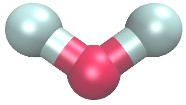
\includegraphics[width=2.4cm]{single_water_LR.jpg}
\caption{
\label{fig:single_water}
Coordinates of a single water molecule in our example.
(Atomic radii not to scale.)
}
\end{figure}

  Here we show an example of a lammps-template file for water.
  %``.lt'' files can store topology and force-field settings in raw LAMMPS format.
(The settings shown here are borrowed from the simple-point-charge 
 \cite{Berendsen++StraatsmaJPhysChem1987} SPC/E model.) 
   %and can be overridden or modified by 
   %combining this LT file with other LT files.)
In addition to coordinates, topology and force-field settings, 
``LT'' files can optionally include any other kind of LAMMPS settings
including SHAKE constraints, k-space settings, and even group definitions.
  %\pagebreak
\begin{verbatim}
# (NOTE: Text following '#' characters are comments)
#
# file "spce_simple.lt" 
#
#    H1     H2
#      \   /
#        O
#

SPCE {

  ## Atom properties and molecular topology go in the various "Data ..." sections

  # We selected "atom_style full".  That means we use this column format:
  # atomID      molID         atomType  charge  coordX    coordY    coordZ

  write("Data Atoms") {
    $atom:o      $mol:.       @atom:O  -0.8476  0.0000000 0.000000  0.00000
    $atom:h1     $mol:.       @atom:H   0.4238  0.8164904 0.5773590 0.00000
    $atom:h2     $mol:.       @atom:H   0.4238  -0.8164904 0.5773590 0.00000
  }

  # Variables beginning with $ or @ will be replaced by numbers LAMMPS will
  # eventually read.  Each of the three atoms" will be assigned unique
  # atomIDs (denoted here by "$atom:o", "$atom:h1", "$atom:h2"), even if
  # they belong to different molecules.  However, the atom types
  # (denoted "@atom:O", "@atom:H") are shared for atoms in all molecules.
  # All 3 atoms share same molID number (represeted here by "$mol:.")
  # however that number is different for different water molecules.

  write_once("Data Masses") {
    # atomType  mass
    @atom:O    15.9994
    @atom:H    1.008
  }

  write("Data Bonds") {
    #  bondID  bondType  atomID1  atomID2
    $bond:oh1  @bond:OH  $atom:o  $atom:h1
    $bond:oh2  @bond:OH  $atom:o  $atom:h2
  }

  write("Data Angles") {
    # angleID  angleType  atomID1  atomID2 atomID3
    $angle:hoh @angle:HOH $atom:h1 $atom:o $atom:h2
  }

  # --- Force-field parameters go in the "In Settings" section: ---

  write_once("In Settings") {
    # -- Non-bonded (Pair) interactions --
    #          atomType1 atomType2  parameter-list (epsilon, sigma)
    pair_coeff  @atom:O  @atom:O    0.1553 3.166 
    pair_coeff  @atom:H  @atom:H    0.0    2.058
    # (mixing rules determine interactions between types @atom:O and @atom:H)

    # -- Bonded interactions --
    #             bondType   parameter list (k_bond, r0)
    bond_coeff   @bond:OH    1000.00 1.0 
    #             angleType  parameter-list (k_theta, theta0)
    angle_coeff  @angle:HOH  1000.0   109.47

    # Group definitions and constraints can also go in the "In Settings" section
    group spce type  @atom:O  @atom:H
    fix fSHAKE spce shake 0.0001 10 100 b @bond:OH a @angle:HOH
    # (lammps quirk: Remember to "unfix fSHAKE" during minimization.)
  }

  # LAMMPS supports a large number of force-field styles. We must select
  # which ones we need. This information belongs in the "In Init" section.

  write_once("In Init") {
    units        real                 # angstroms, kCal/mole, Daltons, Kelvin
    atom_style   full                 # select column format for Atoms section
    pair_style   lj/charmm/coul/long 9.0 10.0 10  # params needed: epsilon sigma
    bond_style   harmonic             # parameters needed: k_bond, r0
    angle_style  harmonic             # parameters needed: k_theta, theta0
    kspace_style pppm 0.0001          # long-range electrostatics sum method
    pair_modify  mix arithmetic       # using Lorenz-Berthelot mixing rules
  }

} # SPCE
\end{verbatim}
Words which are preceded by ``\$'' or ``@'' characters 
are counter variables and will be replaced by integers. 
(See section \ref{sec:variables} for details.)
Users can include SPCE water in their simulations using commands like these:
\begin{verbatim}
# -- file "system.lt" --
import "spce_simple.lt"
wat = new SPCE [1000]
\end{verbatim}
You can now use ``moltemplate.sh'' to create simulation input files for LAMMPS
\begin{verbatim}
moltemplate.sh -pdb coords.pdb -atomstyle "full" system.lt
\end{verbatim}
This command will create lammps input files 
for the molecular system described in ``system.lt'',
using the desired atom style (``full'' by default).
In this example, moltemplate is relying on an external file (``coords.pdb'')
to supply the atomic coordinates of the water molecules, as well as
the periodic boundary conditions.
Coordinates in XYZ format are also supported using ``-xyz coords.xyz''. 

\subsubsection*{\textit{Details}}
\textit{Note that since XYZ files lack boundary information, you must also 
 include a ``Boundary'' section in your ``.lt'' file, as demonstrated 
 in section \ref{sec:pbc}. 
 In both cases, the order of the atom types in a PDB or XYZ file 
 (after sorting) should match the order they are created by moltemplate
 (which is determined by the order of the ``new'' commands 
 in the LT file). 
 Unfortunately this may require careful manual editing of the PDB or XYZ file.}
  %(See appendix \ref{sec:order_customization} for instructions
  % how to customize the order of moltemplate counting).

\subsection{Coordinate generation}
\label{sec:coords_intro}
It is not necessary to provide a separate file with atomic coordinates. 
It is more common to manually specify the location 
(and orientation) of the molecules in your system using the
 ``.move()'' and ``.rot()'' commands %for rigid-body movement 
in the LT file itself 
(discussed in section \ref{sec:coordinates}).
For example you can replace the line:
\begin{verbatim}
wat = new SPCE [1000]
\end{verbatim}
from the example above with 1000 lines:
\begin{verbatim}
wat1    = new SPCE
wat2    = new SPCE.move(3.450, 0.0, 0.0)
wat3    = new SPCE.move(6.900, 0.0, 0.0)
wat4    = new SPCE.move(10.35, 0.0, 0.0)
  :           :
wat1000 = new SPCE.move(34.50, 34.50, 34.50)
\end{verbatim}
Specifying geometry this way is tedious.
Alternatively, moltemplate has simple commands for arranging multiple 
copies of a molecule in periodic, crystalline, toroidal, and helical 
1-D, 2-D, and 3-D lattices.  
For example, you can generate a simple cubic lattice of 
10$\times$10$\times$10 water molecules
(with a 3.45 Angstrom spacing)
using a single command 
(which in this example we split into multiple lines)
\begin{verbatim}
wat  = new SPCE [10].move(0,0,3.45) 
                [10].move(0,3.45,0) 
                [10].move(3.45,0,0)
\end{verbatim}
(See section \ref{sec:coordinates} for more details and examples.)
This will create 1000 molecules with names like
``wat[0][0][0]'', ``wat[0][0][1]'',$\ldots$, ``wat[9][9][9]''.
You can always access individual atomIDs, molIDs, bondIDs, angleIDs, 
and dihedralIDs (if present), for any molecule 
elsewhere in your LT files using this notation:
``\$atom:wat[2][3][4]/h1'', 
``\$bond:wat[0][5][1]/oh1'', 
``\$angle:wat[2][8][3]/hoh'', 
``\$mol:wat[0][1][2]''.
This allows you to define interactions which link
different molecules together (see section \ref{sec:coordinates}).

A list of available coordinate transformations 
is provided in section \ref{sec:xforms_table}.

%\subsubsection*{Defining the simulation boundary}
\subsubsection*{Boundary Conditions:}
\label{sec:pbc}
LAMMPS simulations have finite volume and are usually periodic. 
We must specify the dimensions of the simulation boundary 
using the ``write\_once(``Data Boundary'')'' command.  
\begin{verbatim}
write_once("Data Boundary") {
   0.0  34.5  xlo xhi
   0.0  34.5  ylo yhi
   0.0  34.5  zlo zhi
}
\end{verbatim}
This is usually specified in the outermost LT file 
(``system.lt'' in this example).
\textit{(Note: Boundary conditions do not have to be rectangular 
or even periodic.  For triclinic cells, additional 
``xy'', ``xz'', and ``yz'' tilt parameters can be added.
  %The ``write\_once("In Init") { boundary p p f }'' command 
  %can be used to turn off periodicity in the Z-direction, for example.
For details, lookup the ``read\_data'' and ``boundary'' 
commands in the official LAMMPS documentation.)}

This system is shown in figure \ref{fig:spce_x_1000}a).
After you have specified the geometry, 
then you can run moltemplate.sh this way:
\begin{verbatim}
moltemplate.sh -atomstyle "full" system.lt
\end{verbatim}

\begin{figure}[htbp]
\centering
\textbf{a)}
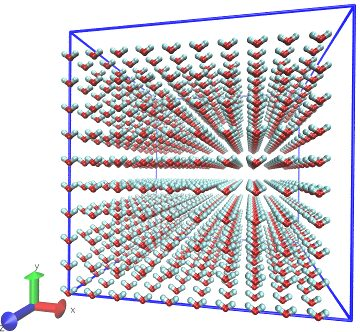
\includegraphics[width=5cm]{waterSPCEx1000_LR.jpg}
\textbf{b)}
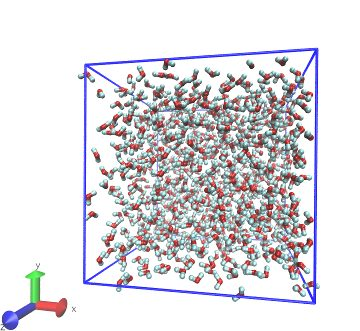
\includegraphics[width=5cm]{waterSPCEx1000_t=25_LR.jpg}
\caption{
\label{fig:spce_x_1000}
A box of 1000 water molecules (before and after pressure equilibration), 
generated by moltemplate and visualized by VMD with the topotools plugin.
(The VMD console commands used for visualization were:
``topo readlammpsdata system.data full'',
``animate write psf system.psf'',
``pbc wrap -compound res -all'', and 
``pbc box''.
See sections \ref{sec:vmd_topotools}, and \ref{sec:vmd_advanced}
for details.
}
\end{figure}

  %\subsubsection*{\textit{Non-periodic simulations}}
  %The use of periodic boundary conditions in LAMMPS is optional.
  %For example the ``boundary p p f'' command turns off 
  %periodic boundary conditions in the Z-direction. 
  %  %When using LAMMPS, commands like this belong 
  %  %near the beginning of a LAMMPS input script.
  %In moltemplate.sh, these kinds of commands go in the ``In Init'' section:
  %\begin{verbatim}
  %write_once("In Init") {
  %  boundary p p f
  %}
  %\end{verbatim}
  %Note that the simulation volume is still finite.

\subsection{Visualization using VMD \& topotools}
\label{sec:vmd_topotools}

When you run moltemplate, it generates a LAMMPS \textit{data} file. 
This file is usually called ``system.data''.
Geometric information, and bonded topology are stored in this file.
After you have run moltemplate, you should look at your system 
to check it for mistakes. 
Problems can easily occur with overlapping atoms (missing molecules), 
periodic boundaries, incorrectly bonded atoms, incorrect rotation and movement.
Sometimes many iterations of running moltemplate and 
visualization are necessary.  

\textit{Optional:}
If you have VMD installed, you can automatically visualize the system
you have just created automatically by invoking moltemplate with 
the \textit{\textbf{-vmd}} command line argument.
(In other words invoke moltemplate.sh using \textit{moltemplate.sh -vmd}
 instead of \textit{moltemplate.sh}.  VMD must be installed.)
If you don't use the -vmd command line argument, you can always view the 
system in VMD later manually.  For instructions how to do that, 
keep reading...

Some very basic instructions how to use VMD are provided below:
\textit{(Note: These instructions were written for VMD 1.9 and topotools 1.2)}
  %See appendix \ref{sec:vmd_advanced} for more details.)

To view a \textit{data} file:
\begin{list}{}
\item a) start VMD
\item b) from the menu, select 
         \textbf{Extensions}$\rightarrow$\mbox{\textbf{Tk Console}} 
\item c) enter:
\end{list}
\begin{verbatim}
        topo readlammpsdata system.data full
        animate write psf system.psf
\end{verbatim}
\begin{list}{}
\item The first command will display all of the atoms and bonds in your system
in VMD's 3-D window.  (We use ``\textbf{full}'' because we are using the 
``full'' atom\_style in this particular example.  If you are using a different 
atom\_style, then change the command above accordingly.)
\item The second command
%\begin{verbatim}
%        \textit{``animate write psf system.psf''},
%\end{verbatim}
will create a PSF file (``system.psf'') which will 
be useful later for viewing a trajectory file created 
during a LAMMPS simulation.
(See section \ref{sec:vmd_trajectory}.)
\end{list}

Most likely, atoms and bonds will be represented by 
ugly dots and lines by default. 
To change the way molecules are displayed, control their color, 
display periodic boundaries, and wrap atomic coordinates,  
read the short VMD tutorial in appendix \ref{sec:vmd_advanced}.

\textit{(Note:
As of 2019-9-03, 
VMD does not have built-in support for exotic atom\_styles 
such as ellipsoids and dipoles, but their are 3rd-party scripts, plugins 
and settings you can use. Search the VMD and LAMMPS mailing lists 
for help.})



\subsection{Running a LAMMPS simulation (after using moltemplate)}
\label{sec:run}
To run a simulation of one or more molecules, 
LAMMPS requires an \textit{input script} and a \textit{data file}.
Input scripts typically contain
force field styles, parameters and run settings.
(They sometimes also contain atom coordinates.)
Data files typically contain atom coordinates and bonded topology data.
(They sometimes also contain force-field parameters.)
  %LAMMPS does strictly not require users to supply a data file, but they 
  %are required for systems with nontrivial bonded molecular topology.

Moltemplate will create the following files: 
``system.data'',
``system.in'',
``system.in.init'',
``system.in.settings'',
(and possibly other files including ``system.in.coords''). 
These are LAMMPS input/data files, and they can be run in LAMMPS 
with minimal modification (see below).
The main input script file is named ``system.in'', and it usually contains
just three lines:
\begin{verbatim}
include   "system.in.init"
read_data "system.data"
include   "system.in.settings"
\end{verbatim}

To \textit{run} a simulation, you will have to 
edit this file in order to add a couple of run commands.  
These commands tell LAMMPS about the simulation conditions
you want to use (temperature, pressure), 
how long to run the simulation,
how to integrate the equations of motion,
and how to write the results to a file (file format, frequency, etc).
Moltemplate.sh can not do this for you.
Some simple examples (which you can paste into your input script)
are provided in the 
\textit{online examples} 
which can be downloaded from \url{http://moltemplate.org}.
  %directories which are bundled with moltemplate.
(These example input scripts 
 typically have names like ``run.in.nvt'' and ``run.in.npt''.)
%below:

   In addition to the examples, an introduction to LAMMP 
input scripts is provided at these links:
\url{http://lammps.sandia.gov/doc/Section_commands.html#cmd_1}.
\url{http://lammps.sandia.gov/doc/Section_howto.html} and 
\url{http://lammps.sandia.gov/doc/Section_howto.html#howto_15}


Here is a list of basic input script commands 
used in the moltemplate examples
(and links to their documentation):
\begin{list}{}
\item \textbf{run} \ 
\url{http://lammps.sandia.gov/doc/run.html}
\item \textbf{timestep} \ 
\url{http://lammps.sandia.gov/doc/timestep.html}
\item \textbf{thermo} \ \url{http://lammps.sandia.gov/doc/thermo.html}
\item \textbf{dump} \ \url{http://lammps.sandia.gov/doc/dump.html}
\item \textbf{read\_data} \ \url{http://lammps.sandia.gov/doc/read_data.html}
\item \textbf{restart} \ \url{http://lammps.sandia.gov/doc/restart.html}
\item \textbf{include} \ \url{http://lammps.sandia.gov/doc/include.html}
\item \textbf{fix nve} \ \url{http://lammps.sandia.gov/doc/fix_nve.html}
\item \textbf{fix nvt} \ \url{http://lammps.sandia.gov/doc/fix_nh.html}
\item \textbf{fix npt} \ \url{http://lammps.sandia.gov/doc/fix_nh.html}
\item \textbf{fix langevin} \ \url{http://lammps.sandia.gov/doc/fix_langevin.html}
\item \textbf{fix} \ \url{http://lammps.sandia.gov/doc/fix.html}
\item \textbf{group} \ \url{http://lammps.sandia.gov/doc/group.html}
\item \textbf{compute} \ \url{http://lammps.sandia.gov/doc/compute.html}
\item \textbf{print} \ \url{http://lammps.sandia.gov/doc/print.html}
\item \textbf{variable} \ \url{http://lammps.sandia.gov/doc/variable.html}
\item \textbf{rerun} \ \url{http://lammps.sandia.gov/doc/rerun.html}
\item \textbf{fix shake} \ \url{http://lammps.sandia.gov/doc/fix_shake.html}
\item \textbf{fix rigid} \ \url{http://lammps.sandia.gov/doc/fix_rigid.html}
\end{list}
In addition, all users should be familiar with the following commands:
(These appear in the ``In Init'' section of most LT files.)
\begin{list}{}
\item \textbf{atom\_style} \ \url{http://lammps.sandia.gov/doc/atom_style.html}
\item \textbf{pair\_style} \ \url{http://lammps.sandia.gov/doc/pair_style.html}
\item \textbf{bond\_style} \ \url{http://lammps.sandia.gov/doc/bond_style.html}
\item \textbf{angle\_style} \ \url{http://lammps.sandia.gov/doc/angle_style.html}
\end{list}


%\subsubsection{An overview of popular LAMMPS run settings}
%  %Alternately you can 
%  %import or include this LT file 
%  %inside another LT file which has these run commands already.
%  % containing the needed run settings.
%  % to the end of this input script file,
%  %OR include this file in a different input script file which has them.
%\begin{verbatim}
%#  -- declare time step for numerical integration --
%timestep 1.0
%\end{verbatim}
%The Nose-Hoover thermostat \& barostat are popular for dense systems 
%(typically liquids, solids, or liquid/solute mixtures).  Choose between:
%\begin{verbatim}
%#  -- run at constant temperature and pressure (Nose Hoover) --
%fix   fxnpt all npt temp 300.0 300.0 100.0 iso 1.0 1.0 1000.0
%\end{verbatim}
%and
%\begin{verbatim}
%#  -- ALTERNATELY run at constant temperature and volume (Nose Hoover) --
%fix   fxnvt all nvt temp 300.0 300.0 500.0 tchain 1
%\end{verbatim}
%The user must also specify what kind of data they want to save, and how
%frequently they want to save it.  Here are some simple examples:
%\begin{verbatim}
%thermo_style custom step temp pe etotal press vol epair ebond eangle edihed
%thermo       500 # time interval for printing out "thermo" data
%dump         1 all custom 2000 traj.lammpstrj id mol type x y z ix iy iz
%\end{verbatim}
%Finally, you must specify the simulation duration.
%\begin{verbatim}
%run 200000
%\end{verbatim}
%  %A detailed description of these steps are not covered in this manual.
%If the starting geometry of your system is unfavorable (high energy) 
%then numerical explosions may result (causing the infamous 
%``Bond/Angle/Dihedral atoms missing on proc'' errors).
%To avoid this, you may want to insert a ``minimize'' command 
%into your input script before the run command.
%\begin{verbatim}
%#  -- minimize --
%minimize 1.0e-5 1.0e-7 1000 10000
%# (Note: Some fixes, for example "shake", interfere with the minimize command.
%#        You can use the "unfix" command to disable them before minimization.)
%\end{verbatim}
%After these modifications, LAMMPS can then be run using: 
%\begin{verbatim}
%lmp_linux -i system.in
%\end{verbatim}
%(Here we are assuming ``lmp\_linux'' is the name of your LAMMPS executable.)
%A detailed explanation of these commands 
%can be found in the LAMMPS Users Manual.
%  %\textit{(Simple examples of LAMMPS script commands may be found in 
%  %comments that appear at the end of ``system.in'' 
%  %files created by moltemplate.sh.)}
%  %(More detailed explanation of these commands 
%  %can be found in the LAMMPS Users Manual.)
%
%Several examples of complete input scripts exist in the 
%``examples'' section of the moltemplate web site at moltemplate.org.
%
%\subsubsection{Recommendations for dilute coarse-grained systems}
%\label{sec:runcg}
%The Nose-Hoover thermostats are a poor choice for 
%dilute systems with a relatively small number of atoms 
%(such as coarse-grained molecules in implicit solvent).
%   %Note: Special care is required for \textit{coarse-grained} systems.
%(The Berendsen thermostat is also not recommended.)
%The Langevin thermostat is available in LAMMPS, 
%however it (currently as of 2019-9-03) requires 
%two ``fix'' commands, as shown below:
%\begin{verbatim}
%#  -- run at constant volume using Langevin dynamics. --
%fix fxlan all langevin 300.0 300.0 5000 48279
%fix fxnve all nve    # (needed by langevin)
%\end{verbatim}
%You may need to adjust the damping parameter (the 3rd numerical argument) 
%to achieve efficient and physically reasonable dynamics 
%\cite{Klimov+ThirumalaiPRL1997}.



  %More detailed instructions for running ``moltemplate.sh'' are provided
  %in appendix \ref{sec:ttree_man_page}.

  %%%%%%% This comment is interesting (?), but no longer relevant: %%%%%%
  %SPCE {
  %# Note: This extra bracketed text augments (not overwrites) 
  %#       the contents of "SPCE {}" defined in "spce_simple.lt".
  %# Note: Here "@atom:O" and "@atom:H" refer to variables which were
  %#       originally defined in "spce_simple.lt".  These variables will be
  %#       numbered consistently as if they belong to the same file
  %}
  %%%%%%%%%%%%%%%%%%%%% --Please Ignore -- %%%%%%%%%%%%%%%%%%%%%%%%%%%%%%
%Later on when we build the final LAMMPS input and data files,
%data from the different files (``Data Atoms'', ``Data Bonds'',
%``In Init'', ``In Settings'', etc...) 
%must be pasted together in the correct order according to LAMMPS conventions.
%This is a simple task that can be performed by the ``moltemplate'' script
%(included with ttree), 
%or manually by the user, depending on their familiarity with LAMMPS.
%LAMMPS has a complex and diverse syntax because 
%it supports a wide variety of force-field types. 
%The commands above are \textit{raw} LAMMPS commands,
%augmented by ttree variables
%(like ``@atom:O'' and ``\$atom:o''), which are explained below.


  %and/or CHARMM27 parameter files.
  %We hope ttree is flexible enough that it should remain useful in the future,
  %even if the LAMMPS input syntax changes radically.

  %\subsection{Before ttree}
  %The ability to load and combine data from multiple different types of 
  %molecules together is missing from LAMMPS. 
  %\textit{Normally} LAMMPS users are required to manually assign unique 
  %id numbers to \textit{every} atom, bonded, 3-body, and 4-body interaction
  %in the entire simulation.  
  %Each molecule is assigned a unique id number as well.
  %For a system with 6000 water molecules, a user would be required to 
  %specify 18000 atom ids, 12000 bond ids, 6000 3-body angle ids
  %and 6000 molecule ids.  
  %(This should not be done by hand.)


\subsection{Visualizing Trajectories}
\label{sec:vmd_trajectory}
After you have run a simulation in LAMMPS, there are several programs which
can visualize the system.
If you have saved your trajectory in LAMMPS ``dump'' format,
later you can view it in VMD \cite{VMD}.
For the purpose of viewing trajectories in LAMMPS, 
I recommend using the following style of ``dump'' commands in the LAMMPS 
input-script that you use when you run LAMMPS:
\begin{verbatim}
dump 1 all custom 1000 DUMP_FILE.lammpstrj id mol type x y z ix iy iz
\end{verbatim}
(The ``all'' and ``1000'', refer to the atom selection and save interval, which may differ depending on the kind of simulation you are running.  See \url{http://lammps.sandia.gov/doc/dump.html} for details.)


Once you have a dump file, you can view it in VMD using:
\begin{list}{}
\item a) Start VMD
  From the menu in the upper-left, select 
  \textbf{File}$\rightarrow$\mbox{\textbf{New Molecule}}
\item b) Browse to select the PSF file you created above, and load it.
  (Don't close the window yet.)
\item c) Browse to select the trajectory file.
  If necessary, for "file type" select: "LAMMPS Trajectory".  
  Click on \textbf{OK}.
\item d) Click on the \textbf{Load} button.
\end{list}


Again, to customize molecule appearance,
display periodic boundary conditions and wrap molecule coordinates,
see the commands discussed in appendix \ref{sec:vmd_advanced}.

\textit{(Note: VMD may not be able to correctly visualize simulations which do
not preserve the number of atoms and bonds over time, such as those run using 
\textbf{fix bond/create}, 
\textbf{fix bond/break}, or
\textbf{fix gcmc}.)}

%\textit{(A note on trajectory format:
%It's a good idea to use an atom\_style which supports molecule-ID numbers 
%(to make it easy to wrap atom coordinates without breaking molecules in half).
%I've been using this command in my LAMMPS scripts to create the trajectories:
%``dump 1 all custom 5000 DUMP\_FILE.lammpstrj id mol type x y z ix iy iz'')}


  %Of course, you don't have to save your trajectories in DUMP format, 
  %(other formats like DCD work fine)  I just mention dump files 
  %because these are the files I'm familiar with.

\section{Overview}
  %This paragraph below is an excellent
  %summary/explanation of what moltemplate.sh does.

\subsection{Basics: The \textit{write()} and \textit{write\_once()} commands}
\label{sec:write}
Each LT file typically contains one or more 
``write'' or ``write\_once'' commands. 
These commands have the following syntax 
\begin{verbatim}
write_once(filename) {text_block}
\end{verbatim}
This creates a new file with the desired file name 
and fills it with the text enclosed in curly brackets \{\}.
  %(after any necessary variable substitutions have been made). 
Text blocks usually span multiple lines and contain counter variables 
(beginning with ``@'' or ``\$'').
which are replaced with numbers.
However the ``write()'' command will repeatedly append the 
same block of text to the file every time the molecule 
(in which the write command appears) is generated or copied 
(using the ``new'' command, 
after incrementing the appropriate counters,
as explained in \ref{sec:instance_variables}).
 %incrementing any counter 
 %variables beginning with \$). 
  %When this happens, any counter variables beginning 
  %with \$ will be incremented.)
%On the other hand, ``write\_once()'' commands print their text only once.
%This is useful in certain cases.  For example, there is no need to redundantly 
%specify the mass of the ``O'' and ``H'' atoms every time you create another copy
%of the same molecule. This kind of data should be written only once using the 
%``write\_once(``Data Masses'')'' command.
   %However, new atoms are generated every time a new copy of a previously 
   %defined molecule is created.  This kind of data should be written using the
   %``write(``Data Atoms'')'' command.


\subsection{Basics: counter variables}
\label{sec:variables}

Words following a ``@'' or a ``\$'' character
are \textit{counter variables}. 
(These are not to be confused with \textit{LAMMPS variables}
 \url{http://lammps.sandia.gov/doc/variable.html}).
By default, 
\textit{all counter variables are substituted with a numeric counter}
before they are written to a file. 
  %(or to a section of a LAMMPS DATA file as 
  %explained in section \ref{sec:write}).
These counters begin at 1 (by default), and 
are incremented as the system size and complexity grows (see below).

These words typically contain a colon (:) followed by more text.
The text preceding this colon is the \textit{category name}. 
(For example: ``\$atom:'', ``\$bond:'', ``\$angle:'', 
     ``@atom:'', ``@bond:'', ``@angle:'') 
Variables belonging to different categories 
are counted independently. 

Users can override these assignment rules and create custom categories.
(See appendices \ref{sec:manual_assignment} and \ref{sec:custom_categories}
for details.)

\subsubsection{Static counters begin with ``@''}
\label{sec:static_variables}

``@'' variables generally correspond to \textit{types}: 
such as atom types, bond types, angle types, dihedral types, improper types.
These are simple variables and they assigned to unique integers in the 
order they are read from your LT files.
Each uniquely named variable in each category is assigned to a different 
integer.  For example, ``@bond:'' type variables are numbered from ``1''
to the number of \textit{bond types}.
(Pairs of bonded atoms are assigned a \textit{bond type}. 
Later, LAMMPS will use this integer to lookup the bond-length and Hooke's-law 
elastic constant describing the force between these two atoms.)

%These numbers do not change if the number of molecule copies 
%increases.

\subsubsection{Instance counters begin with ``\$''}
\label{sec:instance_variables}

On the other hand, ``\$'' variables correspond 
to unique ID numbers: atom-IDs, bond-IDs,
angle-IDs, dihedral-IDs, improper-IDs, and molecule-IDs.  These
variables are created whenever a copy of a molecule is created (using
the ``new'' command).  
If you create 1000 copies of a water molecule using a command like 
\begin{verbatim}
wat = new SPCE[10][10][10]
\end{verbatim}
then moltemplate creates 3000 ``\$atom'' variables with names like
\begin{verbatim}
$atom:wat[0][0][0]/o
$atom:wat[0][0][0]/h1
$atom:wat[0][0][0]/h2
$atom:wat[0][0][1]/o
$atom:wat[0][0][1]/h1
$atom:wat[0][0][1]/h2
\end{verbatim}
$\quad \vdots $
\begin{verbatim}
$atom:wat[9][9][9]/o
$atom:wat[9][9][9]/h1
$atom:wat[9][9][9]/h2
\end{verbatim}

\subsubsection{Variable names: short-names \textit{vs.} full-names}
\label{sec:full_names}

In the example above, the \$ variables have full-names like
``\$atom:wat[8][3][7]/h1'', not ``\$atom:h1''.  However inside the
definition of the water molecule, you don't specify the full name.
You can refer to this atom as ``\$atom:h1''.
Likewise, the full-name for the @atom variables is actually
``@atom:SPCE/H'', not ``@atom:H''.  However inside the definition of the water
molecule, you typically use the shorthand notation ``@atom:H''.

\subsubsection{Numeric substitution}
Before being written to a file, every variable (either \$ or @) 
with a unique \textit{full-name} will be assigned to a unique integer, 
starting at 1 by default.
  %(You can override this choice if you want to using the "-a" flag.)

The various \$atom variables in the water example will be substituted 
with integers from 1 to 3000 (assuming no other molecules are present).
But the ``@atom:O'' and ``@atom:H'' variables
(which are shorthand for ``@atom:SPCE/O'' and ``@atom:SPCE/H'')
will be assigned to to ``1'' and ``2''
(again, assuming no other molecule types are present).

So, in summary, @ variables increase with the \textit{complexity} 
of your system
(IE the number of molecule types or force-field parameters), 
but \$ variables increase with the \textit{size} of your system.

\subsubsection{Variable scope}
\label{sec:variable_scope}
This effectively means that all variables are specific to
local molecules they were defined in.
In other words, an atom type named ``@atom:H'' inside 
the ``SPCE'' molecule, will be assigned to a different number
than an atom named ``@atom:H'' in an ``Arginine'' molecule.
This is because the two variables will have different \textit{full} names
(``@atom:SPCE/H'', and ``@atom:Arginine/H'').







\subsubsection*{Sharing atom types or other variables between molecules}
There are several ways to share atom types between two molecules.
The \textit{recommended way} is to define them in a separate
file and refer to them when needed.
This approach is demonstrated in section \ref{sec:2bead}.

\textit{(Alternately, you can define them outside the current molecule definition,
and use file-system-path-like syntax 
(``../'', or ``../../'' or ``/'')
to access atoms (or molecules) outside of the current molecule.
   %(or nested within the definition of another molecule).
For example, two different molecule types can share the same type of
hydrogen atom by referring to it using this syntax: ``@atom:../H''.
  %(Two molecules could share the same atom-id in a similar way, 
  % using ``\$atom:../h1''.  This is not recommended)
For details, see
section \ref{sec:paths}.
and appendix \ref{sec:adv_variable_syntax}.)
  %To be on the safe side, if you want to define a single 
  %hydrogen atom type named ``H'' globally, for example, 
  %then you would refer to this atom everywhere using ``@atom:/H''.
  %(A more portable alternative would be to use the ``@atom:.../H'' 
  % syntax explained in appendix \ref{sec:adv_variable_syntax}.
  % This is similar to ``@atom:/H'',
  % however using the ellipsis syntax ``@atom:.../H'' allows you to 
  % share your molecule definitions (ET files) with others 
  % who may have a different notion of what the ``H'' atom is.)
}





\subsection{Troubleshooting using the \textit{output\_ttree} directory}
\label{sec:output_ttree}
Users can see what numbers were assigned to each variable 
by inspecting the contents of the ``output\_ttree'' subdirectory
created by moltemplate. 
Unfortunately, it not unusual for LAMMPS to crash the first time you 
attempt to run it on a DATA file created by moltemplate.  This often occurs 
if you failed to spell atom types and other variables consistently.
The LAMMPS error message (located at the end of the ``log.lammps''
file created by LAMMPS) will help you determine what type of mistake you made.
(For example, what type of variable was misspelled or placed in the wrong place?)


To help you, the ``output\_ttree'' directory contains a file named 
``ttree\_assignments.txt''. 
This is a simple 2-column text file containing a list of \textit{all} 
of the variables you have created in one column, and the numbers they
were assigned to in the second column.
(There is also a comment on each line beginning with a ``\#'' character which
indicates the file and line number where this variable is first used.)

The ``output\_ttree'' directory also contains all of the files that you created.
The versions with a ``.template'' extension contain text
interspersed with \textit{full} variable names (before numeric substitution).
(A spelling mistake, like using ``\$atom:h'' when you meant to say ``\$atom:h1''
or ``@atom:H'' will show up in these files if you inspect them carefully.)
This can help you identify where the mistake occurred
in your LT files.

Once a molecular system is debugged and working, users 
can ignore or discard the contents of this directory.


\subsection{``Data'' and ``In''}
\label{sec:DataIn}
Again, LAMMPS requires an \textit{input script} and a \textit{data file} 
to run.    
\textit{Moltemplate's job is to generate these files.}
\textit{Input scripts} typically contain
force-field styles, parameters and run settings
  %Moltemplate users control what goes in the input script
  %by writing to files with names beginning with \mbox{``In ''}.
\textit{Data files} typically contain atom 
coordinates and bonded topology data.
  %Moltemplate users control what goes in the data file
  %by writing to files with names beginning with \mbox{``Data ''}.

If you are familiar with LAMMPS, 
you may have noticed the file names above
(in the example from section \ref{sec:spce_example})
sound suspiciously like sections from LAMMPS data files or input scripts, 
such as ``Data Boundary'', ``Data Atoms'', ``Data Bonds'', ``Data Masses'', ``Data Angles'', ``Data Dihedrals'', ``Data Impropers'', ``In Init'', ``In Settings'').
All files whose names begin with ``In '' or ``Data '' are special.
For the user's convenience, 
the moltemplate.sh script copies the contents 
of these files into the corresponding section 
(``Atoms'', ``Bonds'', ``Angles'', etc.)
of the 
DATA file or INPUT scripts generated by moltemplate 
(``system.data'', ``system.in.settings'', etc).
(Then the original files are moved to the ``output\_ttree/'' directory, 
 in an effort to clean things up and hide them from view.)
Users can create their own custom sections to a LAMMPS data file.
(See section \ref{sec:custom_data}.
   %(Note: It is unwise to explicitly add blank lines to a data file section.
   %because LAMMPS may interpret them as section breaks. 
   %Moltemplate will add the section headers 
   %and blank lines needed to keep LAMMPS happy.)

More generally, the ``write()'' and ``write\_once()'' commands can be used to
create any other files you may need to run your simulations,
which refer to the same \textit{@atom} and \textit{@bond} types.
   %Files whose names do not begin with ``In '' or ``Data '' can have any format
   %(and are not moved or cleaned up).
   %(These files are not removed or hidden later.) 
(See section \ref{sec:aux_files} 
  % and \ref{sec:output_ttree} for examples
for an example.)


\subsection{\textit{(Advanced)} 
               Using moltemplate to generate auxiliary files}
\label{sec:aux_files}
The following excerpt from an LT file 
creates a file named ``system.in.sw''. 
(It contains parameters for the ``sw'' pair style.
 This exotic many-body pair style requires a large number
 of parameters, which are read from a separate file.)
This ``system.in.sw'' file file will be read later when you run the simulation.
(The pair\_coeff command below tells LAMPS to read that file.)
\begin{verbatim}
write_once("system.in.sw") {
  mW mW mW 6.189 2.3925 1.8 23.15 1.2 -0.33333 7.04956 0.602224 4 0 0
}
write_once("In Settings") {
  pair_coeff * * sw system.in.sw mW NULL NULL NULL
}
\end{verbatim}
As new force-field styles and/or fixes are added to LAMMPS, 
the files they depend on can be embedded in an LT file in this way. 


\subsection{\textit{(Advanced)} Making custom DATA sections}
\label{sec:custom_data}
Suppose that in the future, the format of the LAMMPS DATA file changes
so that it now becomes necessary to supply a new section named ``Foo Fee Fum'',
for example.  You could do that using this command:
\begin{verbatim}
write_once("Data Foo Fee Fum") {
  File contents goes here. (These files can contain
  atom counters and/or other counter variables).
}
\end{verbatim}
This way moltemplate copy this text into the ``Foo Fee Fum'' section at
the end of the DATA file it is constructing.
This allows users to adapt to future changes in the LAMMPS data file format.



\subsubsection*{Does ``@atom:H'' conflict with ``\$atom:H''?}
\label{sec:vardetails}
No.  It is okay for static(@) and instance(\$) variables to share the same names.
(Moltemplate considers them distinct variables and they will be assigned independently.)


\subsubsection*{Addional Details}
Variable and molecule names can include unicode characters.
They can also include some whitespace characters and other special characters
by using backslashes and curly-brackets, for example:
``@\{atom: CA \}'' and ``@atom:\textbackslash\ CA\textbackslash\ ''.
Curly-brackets are useful to clarify when a variable name begins and ends,
such as in this example: ``@\{atom:C\}*@\{atom:H\}''.
This prevents the ``*'' character from being appended to the end of the 
``C'' variable name.
(Note that using the ``*'' character in any of the \textit{coeff} commands
within moltemplate is discouraged.  See section \ref{sec:wildcard_bug}.)

\textit{(Unicode is supported.)}


\pagebreak
\section{ Object composition and coordinate generation }
\label{sec:coordinates}

Objects can be connected together to form larger molecule objects.
These objects can be used to form still larger objects.
As an example, we define a small 2-atom molecule named ``Monomer'',
and use it to construct a short polymer (``Polymer'').

\begin{figure}[htbp]
\centering
\textbf{a)}
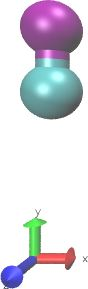
\includegraphics[height=3cm]{2bead_monomer.jpg}
\quad \quad \quad \quad \quad
\textbf{b)}
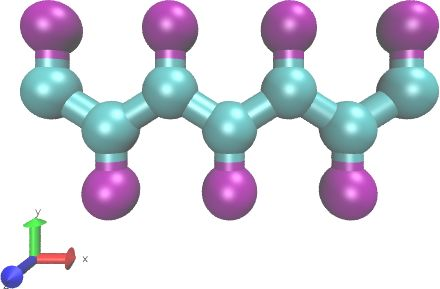
\includegraphics[height=3cm]{2bead_polymer.jpg}
\newline
\vspace{10 mm}
\newline
\textbf{c)}
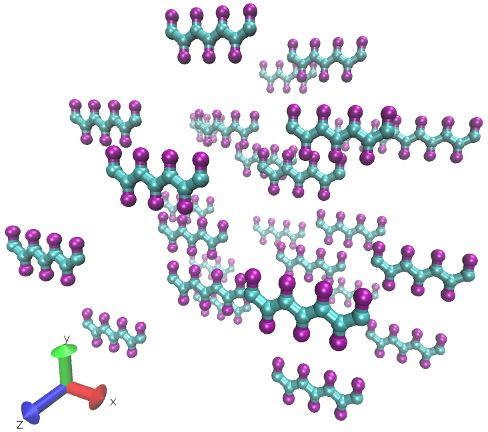
\includegraphics[width=4cm]{2bead_polymers_nopbc_t=0_LR.jpg}
\textbf{d)}
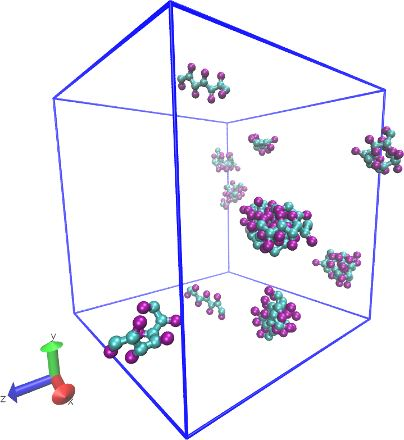
\includegraphics[width=4cm]{2bead_polymers_t=100ps_LR.jpg}
\caption{
\label{fig:2bead_polymer}
\textbf{a)-b)}
\textit{Building a complex system from small pieces:}
Construction of a polymer (\textbf{b}) 
out of smaller (2-atom) subunits (\textbf{a})
using composition and rigid-body transformations. 
Bonds connecting different monomer together (blue) 
must be declared explicitly, 
but angle and dihedral interactions will be generated automatically.
See section \ref{sec:2bead} for details.
\textbf{c)}
An irregular lattice of short polymers.
(See section \ref{sec:multidimensional_arrays}.)
\textbf{d)}
The same system after 100000 time steps using Langevin dynamics.
  %the Langevin dynamics settings from section \ref{sec:runcg}.
(The VMD console commands used for visualization were:
``topo readlammpsdata system.data full'',
``animate write psf system.psf'',
``pbc wrap -compound res -all'', and 
``pbc box''.
See sections \ref{sec:vmd_topotools}, and \ref{sec:vmd_advanced}
for details.}
\end{figure}



\pagebreak

\subsection{Building a large molecule from smaller pieces}
\label{sec:2bead}
Consider the following simple 2-atom dumbell-shaped molelule (``Monomer'')
\begin{verbatim}
# -- file "monomer.lt" --

import "forcefield.lt"   # contains force-field parameters

Monomer inherits ForceField {

  write("Data Atoms") {
    # atomId molId   atomType   charge   x      y        z      
    $atom:ca $mol:... @atom:CA   0.0   0.000  1.0000   0.0000000
    $atom:r  $mol:... @atom:R    0.0   0.000  4.4000   0.0000000
  }
  write("Data Bonds") {
    # bond-id   bond-type        atom-id1  atom-id2
    $bond:cr    @bond:Sidechain  $atom:ca  $atom:r
  }
}
\end{verbatim}


Soon will use it to construct a polymer (``Polymer'')
\textit{Note: The ellipsis notation used here ``\$mol:...''.
warns moltemplate that the ``Monomer'' molecule may be part of a larger
molecule.
(This is explained in more detail in section \ref{sec:ellipsis_mol}.)
(Note: The meaning of ``inherits ForceField''
       will be explained below in section \ref{sec:nbody_by_type_intro})
}
       
In this example we will define two kinds of molecule objects:
``Monomer'', and ``Polymer'' (\textit{defined later}).

\subsubsection*{Building a simple polymer}
We construct a short polymer by making 7 copies of ``Monomer'',
rotating and moving each copy:
\label{sec:2beadPolymer}
\begin{verbatim}
# -- file "polymer.lt" --

import "monomer.lt"  #(defines "Monomer" and "ForceField")

Polymer inherits ForceField {

  # The next line is optional:
  create_var {$mol}  #(force all monomers to share the same molecule-ID)

  # Now create some monomers

  mon1 = new Monomer     #(no need to move the first monomer)
  mon2 = new Monomer.rot(180.0, 1,0,0).move(3.2,0,0)
  mon3 = new Monomer.rot(360.0, 1,0,0).move(6.4,0,0)
  mon4 = new Monomer.rot(540.0, 1,0,0).move(9.6,0,0)
  mon5 = new Monomer.rot(720.0, 1,0,0).move(12.8,0,0)
  mon6 = new Monomer.rot(900.0, 1,0,0).move(16.0,0,0)
  mon7 = new Monomer.rot(1080.0, 1,0,0).move(19.2,0,0)

  # Now, link the monomers together this way:
  write("Data Bonds") {
    $bond:backbone1  @bond:Backbone  $atom:mon1/ca  $atom:mon2/ca
    $bond:backbone2  @bond:Backbone  $atom:mon2/ca  $atom:mon3/ca
    $bond:backbone3  @bond:Backbone  $atom:mon3/ca  $atom:mon4/ca
    $bond:backbone4  @bond:Backbone  $atom:mon4/ca  $atom:mon5/ca
    $bond:backbone5  @bond:Backbone  $atom:mon5/ca  $atom:mon6/ca
    $bond:backbone6  @bond:Backbone  $atom:mon6/ca  $atom:mon7/ca
  }
}
\end{verbatim}
The position and orientation of each copy of ``Monomer'' 
is specified after the ``new'' statement. 
Each ``new'' statement is typically followed by a chain of 
move/rotate/scale functions separated by dots, evaluated left-to-right
(optionally followed by square brackets and then more dots). 
For example, ``mon2'' is a copy of ``Monomer'' which is first rotated 
180 degrees around the X axis (denoted by ``1,0,0''), 
and \textbf{then} moved in the (3.2,0,0) direction.
(The last three arguments to the ``rot()'' command 
 denote the axis of rotation, which does not have to be normalized.)
(A list of available coordinate transformations 
is provided in section \ref{sec:xforms_table}.)

\textit{(Note: Although we did not do this here, 
it is sometimes convenient to represent polymers as 1-dimensional arrays. 
See sections \ref{sec:arrays} and \ref{sec:random_arrays} for examples.)}

To bond atoms in different molecules or molecular subunits together, we used 
the write(``Data Bonds'') command to append additional bonds to the system.

%\subsubsection{Sharing atom, bond and angle types}
%Normally you must separately define the parameters for all of the atoms types,
%and bond types, angle types etc... in every type of molecule.
%However different kinds of monomers in a heteropolymer typically will 
%share some common backbone atom types and other properties.
%You must be careful to indicate which atom and bond types are shared between
%different monomers by referring them using a ``../'' prefix.
%(See sections \ref{sec:variable_scope}, 
%\ref{sec:paths}, and 
%\ref{sec:butane} for details and examples.)
%\textit{Note: There is a heteropolymer example in the the 
%``2bead\_heteropolymer/'' directory in the online examples.
%This example demonstrates how to share backbone atoms, bonds, and angles. 
%You can also define specific angle or dihedral interactions which are
%specific to the atom types in different monomers.}


\subsection{Bonded interactions \textit{by type}}
\label{sec:nbody_by_type_intro}

In this example we did \textit{not} provide a list of all 3-body
and 4-body angle forces between bonded atoms in the polymer.
Moltemplate allows you to manually list all of these interactions
(using the ``write\_once("Data Angles")'' command
from section \ref{sec:spce_example},
\textit{or} 
the ``write\_once("Data Dihedrals")'', 
or ``write\_once("Data Impropers")'' commands).
However there are usually many of them.
For this reason, it is often more convenient to provide
moltemplate with instructions to help it automatically figure out 
which atoms participate in 3-body and 4-body angle interactions,
and what force field parameters to assign to them.
We will do that below using the following commands:
``write\_once("Data Angles By Type")'',
``write\_once("Data Dihedrals By Type")'', and
``write\_once("Data Impropers By Type")''

  %Moltemplate can detect consecutively bonded atoms and 
  %determine the forces between them based on atom type (and bond type).

Furthermoree, since many different kinds molecules often share
the same rules for creating 3-body and 4-body angle interactions,
it is convenient to organize all of this information
together into one place (eg an object named ``ForceField'').
A ``ForceField'' object will typically include many
``write\_once("Data Angles By Type")''
commands, as well as force field parameters and related atom type properties.
We also typically store that information in a separate file
(eg ``forcefield.lt'', ``oplsaa.lt'', ``gaff2.lt'', ``compass.lt'', etc...).

\begin{verbatim}
# -- file "forcefield.lt" --

ForceField {

  # There are 2 atom types: "CA" and "R"
  write_once("Data Masses") {
    @atom:CA    13.0
    @atom:R     50.0
  }

  # Force-field parameters ("coeffs") go in the "In Settings" section:

  write_once("In Settings") {
    # Pairwise (non-bonded) interactions:
    #           atomType1 atomType2   epsilon sigma
    pair_coeff   @atom:CA @atom:CA       0.10 2.0
    pair_coeff   @atom:R  @atom:R        0.50 3.6
    # (Interactions between different atoms are determined by mixing rules.)
  }

  # 2-body (bonded) interactions:
  #
  #   Ubond(r) = k*(r-r0)^2
  #
  write_once("In Settings") {
    #             bond-type        k     r0
    bond_coeff  @bond:Sidechain   15.0   3.4
    bond_coeff  @bond:Backbone    15.0   3.7
  }

  # Although the simple "Monomer" object we defined above has only
  # two atoms, later on, we will create molecules with many bonds.
  # By convention, in this file we keep track of all of the possible
  # interactions which could exist between these atoms:

  # Rules for determining 3-body (angle) interactions by atom & bond type:
  # angle-type     atomType1 atomType2 atomType3  bondType1 bondType2

  write_once("Data Angles By Type") {
    @angle:Backbone  @atom:CA  @atom:CA  @atom:CA   @bond:*   @bond:*
    @angle:Sidechain @atom:CA  @atom:CA  @atom:R    @bond:*   @bond:*
  }

  # Force-field parameters for 3-body (angle) interactions:
  #
  #   Uangle(theta) = k*(theta-theta0)^2
  #
  write_once("In Settings") {
    #             angle-type       k    theta0
    angle_coeff @angle:Backbone   30.00  114
    angle_coeff @angle:Sidechain  30.00  132
  }

  # 4-body interactions in this example are listed by atomType
  # Rules for determining 4-body (dihedral) interactions by atom & bond type:
  write_once("Data Dihedrals By Type") {
    # dihedralType atmType1 atmType2 atmType3 atmType4 bondType1 bType2 bType3
    @dihedral:CCCC @atom:CA @atom:CA @atom:CA @atom:CA  @bond:* @bond:* @bond:*
    @dihedral:RCCR @atom:R  @atom:CA @atom:CA @atom:R   @bond:* @bond:* @bond:*
  }

  # The forumula used is:
  #
  # Udihedral(phi) = K * (1 + cos(n*phi - d))
  #
  #     The d parameter is in degrees, K is in kcal/mol/rad^2.
  #
  # The corresponding command is 
  # dihedral_coeff dihedralType       K  n   d  w(ignored)

  write_once("In Settings") {
    dihedral_coeff @dihedral:CCCC   -0.5 1 -180 0.0
    dihedral_coeff @dihedral:RCCR   -1.5 1 -180 0.0
  }

  write_once("In Init") {
    # -- Styles used in "ForceField" --
    # -- (Changing these styles will change the formulas above) --
    units           real
    atom_style      full
    bond_style      harmonic
    angle_style     harmonic
    dihedral_style  charmm
    pair_style      lj/cut 11.0
  }
}
\end{verbatim}
Any molecule that wants to access this information can use the
``inherits ForceField'' keyword.
\textit{(...as we did in the ``monomer.lt'' and ``polymer.lt'' files in theexample above.
 Note: the ``import forcefield'' statement was also necessary because the
 information is located in a separate file: ``forcefield.lt''.}
%\textit{(Note: You can also generate \textbf{improper} interactions 
%  %between any 4-atoms bonded together in a T-shaped topology
%  the same way, using the  ``write\_once("Impropers By Type")'' command.
%  See appendix \ref{sec:nbody_by_type} for more details.
\textit{You can customize these ``By Type'' rules further
  by altering the bond topology search rules and atom type symmetry.
  See appendix \ref{sec:nbody_by_type_custom} for details.)}

  %\subsubsection*{\textit{(Advanced)} Order matters when sets overlap}
  %Bonded-interactions are generated in the order they appear in the LT file.
  %Interactions which are declared later may override the settings of 
  %interactions which appear earlier, such as in this example:
  %\begin{verbatim}
  %  write_once("Data Angles By Type") {
  %    @angle:Backbone  @atom:C* @atom:C*  @atom:*    @bond:*   @bond:*
  %    @angle:Sidechain @atom:CA @atom:CA  @atom:R    @bond:*   @bond:*
  %  }
  %\end{verbatim}
  % %Here the first line of this file creates a 3-body angle interaction
  % %of type ``@angle:Backbone'' between \textit{every} triplet of bonded atoms 
  % %in the molecule whose first two atom types begin with the letter ``C''.
  %The second line creates 3body interactions (of type ``@angle:Sidechain'')
  %specifically between atoms of type ``@atom:CA'', ``@atom:CA'', and 
  %``@atom:R'', overriding any triplets of this type which appeared earlier.



%\subsection*{\textit{(Advanced)} Mixing regular and ``By Type'' interactions}

%If an LT file contains both ``Data Angles'' and ``Data Angles By Type'',
%then the interactions explicitly defined in the ``Angles'' section will 
%always override the assignments made in ``Data Angles By Type''.
%The also applies to Dihedrals and Impropers.

  %\begin{verbatim}
  %write("Data Angles") {
  %  $angle:1 @angle:CCCgeneral $atom:c1 $atom:c2 $atom:c3
  %  $angle:2 @angle:CCCgeneral $atom:c1 $atom:c3 $atom:c4
  %}
  %\end{verbatim}


\section{Arrays, slices, and coordinate transformations}
\label{sec:arrays}
Moltemplate supports 1-dimensional, and multi-dimensional arrays.
These can be used to create straight (or helical) polymers
sheets, tubes, tori.
They are also to fill solid 3-dimensional volumes
with molecules or atoms.
(See sections \ref{sec:coords_intro} and \ref{sec:multidimensional_arrays}.)

Here we show an easier way to create the short polymer 
shown in section \ref{sec:2beadPolymer}.
You can make 7 copies of the \textit{Monomer} molecule this way:
\begin{verbatim}
  monomers = new Monomer[7]
\end{verbatim}
This creates 7 new \textit{Monomer} molecules (named 
\mbox{\textit{monomers[0]}}, 
\mbox{\textit{monomers[1]}}, 
\mbox{\textit{monomers[2]}}, 
\mbox{\textit{monomers[3]}}, ... 
\mbox{\textit{monomers[6]}}).
You can connect them with bonds in the same way we did earlier:
\begin{verbatim}
  write("Data Bonds") {
    $bond:backbone1  @bond:Backbone  $atom:monomers[0]/ca  $atom:monomers[1]/ca
    $bond:backbone2  @bond:Backbone  $atom:monomers[1]/ca  $atom:monomers[2]/ca
    $bond:backbone3  @bond:Backbone  $atom:monomers[2]/ca  $atom:monomers[3]/ca
         :                :               :                     :
  }
\end{verbatim}

Unfortunately, by default, the coordinates of each molecule are identical.
To prevent the atom coordinates from overlapping, you have several choices:

\subsection{Transformations following brackets [] in a new statement}
\label{sec:arrays+xform}
   After every square-bracket [] in a new command,
you can specify a list of transformations to apply.
For example, we could have generated atomic coordinates for the 
the short polymer in section \ref{sec:2beadPolymer}
using this command:
\begin{verbatim}
  monomers = new Monomer [7].rot(180, 1,0,0).move(3.2,0,0)
\end{verbatim}
This will create 7 molecules.  
The coordinates of the first molecule \textit{monomers[0]} are will be unmodified.
However each successive molecule will have its coordinates cumulatively
modified by the commands ``rot(180, 1,0,0)'' followed by ``move(3.2,0,0)''.
\subsubsection*{optional: initial customizations (preceding [] brackets)}
\label{sec:xform+arrays+xform} 
You can also make adjustments to the initial coordinates of the molecule
before it is copied, and before any of the array transformations are applied.
For example:
\begin{verbatim}
  monomers = new Monomer.scale(1.5) [7].rot(180, 1,0,0).move(3.2,0,0)
\end{verbatim}
In this example, the ``scale(1.5)'' transformation is applied once to 
enlarge every \textit{Monomer} object initially.
This will happen before any of the rotation and move commands 
are applied to build the polymer
(so the 3.2 Angstrom spacings between each monomer will not be effected).

\subsection{Transformations following instantiation}
\label{sec:xform_after_instance}
Alternately you apply transformations to a molecule 
after they have been created (even if they are part of an array).
\begin{verbatim}
  monomers = new Monomer [7]

  # Again, the first line creates the molecules named 
  # "monomers[0]", "monomers[1]", "monomers[2]", ... "monomers[6]".
  # The following lines move them into position.
  monomers[1].rot(180.0, 1,0,0).move(3.2,0,0)
  monomers[2].rot(360.0, 1,0,0).move(6.4,0,0)
  monomers[3].rot(540.0, 1,0,0).move(9.6,0,0)
  monomers[4].rot(720.0, 1,0,0).move(12.8,0,0)
  monomers[5].rot(900.0, 1,0,0).move(16.0,0,0)
  monomers[6].rot(1080.0, 1,0,0).move(19.2,0,0)
\end{verbatim}

\subsection{Transformation order (general case)}
\label{sec:xform_order}
A typical array of molecules might be instantiated this way:
\begin{verbatim}
mols = new Molecule.XFORMS1() [N].XFORMS2()
mols[*].XFORMS3()
\end{verbatim}
The list of transformations denoted by ``XFORMS1'' in this example
are applied to the molecule first.
Then the transformations in ``XFORMS2'' are then applied to each
copy of the molecule multiple times.  
(For the molecule with index ``$i$'', named ``Molecule[$i$]'',
XFORMS2 will be applied $i$ times.)
Finally after all the molecules have been created, the list
of transformations in XFORMS3 will be applied.
For example, to create a ring of 10 polymers of radius 30.0, 
centered at position (0,25,0), use this notation:
\begin{verbatim}
polymer_ring = new Polymer.move(0,30,0) [10].rot(36,1,0,0)
  # After creating it, we can move the entire ring 
  # (These commands are applied last.)
polymer_ring[*].move(0,25,0)
\end{verbatim}


\subsection{Random arrays}
\label{sec:random_arrays}

\begin{figure}[htbp]
\centering
\textbf{a)}

\includegraphics[height=1.2cm]{random_2bead.jpg}
\hspace{0.2cm}
\textbf{b)}
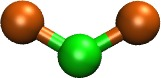
\includegraphics[height=0.75cm]{random_3bead.jpg}
\hspace{0.2cm}
\textbf{c)}
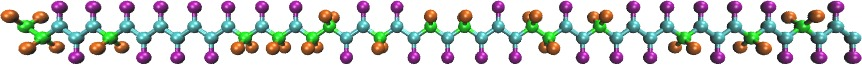
\includegraphics[width=8cm]{random_heteropolymer.jpg}
%\newline
%\vspace{10 mm}
%\newline
\caption{
\label{fig:random_heteropolymer}
A random heteropolymer (\textbf{c}),
composed of of \textit{Monomer} and \textit{Monomer3} monomer subunits
(\textbf{a} and \textbf{b}) with (target) probabilities 0.6 and 0.4.
(However, due to random fluctuations, the actual ratio 
 in this case was 68\% and 32\%.
 To avoid this problem, see section \ref{sec:random_exact}.)
}
\end{figure}
Arrays of random molecules can be generated using the 
\mbox{\textit{new random() []}} syntax.  For example,
below we define a random polymer composed of 50 
\textit{Monomer} and \textit{Monomer3} monomer subunits.
(See figure \ref{fig:random_heteropolymer}.)
\begin{verbatim}
RandPoly50 inherits ForceField {
  # Make a chain of randomly chosen monomers:

  monomers = new random([Monomer, Monomer3], [0.6, 0.4], 123456)
                 [50].rot(180,1,0,0).move(2.95, 0, 0)

  # Now, link the monomers together this way:
  write("Data Bonds") {
    $bond:bb1 @bond:Backbone $atom:monomers[0]/ca $atom:monomers[1]/ca
    $bond:bb2 @bond:Backbone $atom:monomers[1]/ca $atom:monomers[2]/ca
    $bond:bb3 @bond:Backbone $atom:monomers[2]/ca $atom:monomers[3]/ca
    $bond:bb4 @bond:Backbone $atom:monomers[3]/ca $atom:monomers[4]/ca
\end{verbatim}
$\quad \quad \quad \vdots $
%           :           :              :                     :
\begin{verbatim}
    $bond:bb50 @bond:Backbone $atom:monomers[48]/ca $atom:monomers[49]/ca
  }
  #(Note: Both the "Monomer" and "Monomer3" subunits contain atoms
  #       named "$atom:ca".
} #RandPoly50
\end{verbatim}
It is also possible to fill a 2 or 3-dimensional volume with
molecules randomly.  This is discussed in section
\ref{sec:random_advanced}.

%\textit{Note: To specify the exactly number of molecules of each type,
%you can also use this notation (discussed below).}
%\begin{verbatim}
%  monomers = new random([Monomer, Monomer3], [30, 20], 123456)
%                 [50].rot(180,1,0,0).move(2.95, 0, 0)
%\end{verbatim}


The \mbox{\textit{new random()}} function takes 2 or 3 arguments:
a list of molecule types 
(\mbox{\textit{Monomer}} and \mbox{\textit{Monomer3}} in this example),
and a list of probabilities (\textit{0.6} and \textit{0.4})
both enclosed in square-brackets [].

\subsubsection{Random arrays with exact molecule type counts}
\label{sec:random_exact}
Recall that we requested that 60\% of the molecules be of type
``Monomer'' and 40\% type ``Monomer3'' (corresponding to 30 and 20, respectively).
However, the resulting polymer (shown in figure \ref{fig:random_heteropolymer})
contains 34 ``Monomer'' and 16 ``Monomer3'' monomers (68\% and 34\%, respectively).
This is because each time a monomer is created, a random number is generated
to decide which type of monomer will be created.
There is no guarantee that the total final fraction of monomers will 
match the target probabilities exactly (60\% and 40\%, respectively).
To specify the number of molecule types precisely, you can replace 
the list of probabilities ``[0.6,0.4]''
with a list of integers ``[30,20]''.
\begin{verbatim}
  monomers = new random([Monomer, Monomer3], [30, 20], 123456)
                 [50].rot(180,1,0,0).move(2.95, 0, 0)
\end{verbatim}
This will create exactly 30 ``Monomer'' and 20 ``Monomer3'' monomers.
(You can do this with multidimensional arrays as well.  
See section \ref{sec:random_multidim_exact}.)
%(In both case, the sum of the molecule type counts (30,20) must match the 
%number of molecules in the array being created.)


\subsubsection*{Details regarding the \textit{new random} command:}

\textit{Note:} You can tell moltemplate to customize the bond-types and 
              angles, depending on the (types of) monomers are connected
              by each bond.  The ``random\_heteropolymer'' example
              downloadable at \url{www.moltemplate.org} demonstrates
              how to do this.

\textit{Note:}
Although this example, there are only two monomer types
(``Monomer'' and ``Monomer3''), there is no limit to the number 
of molecule types which appear in these lists (eg ``[Monomer, Monomer3, 4bead],[0.2,0.3,0.2]'')

\textit{Note:}
An optional random-seed argument can also be included.
(For example the \mbox{\textit{``123456''}} shown above.
 If you omit this number, then you will get different 
 results each time you run moltemplate.)

\textit{Note:}
These lists can also contain vacancies/blanks.
See section \ref{sec:random_vacancies}.)

\textit{Note:}
Once a molecule containing random monomers is defined, 
(\mbox{\textit{``RandPoly50''}} in this example), each copy of that molecule 
(created using the \textit{new} command) is identical.

\subsubsection*{Optional: Customizing molecule positions 
                          in a \textit{random()} array}
You can customize the position of each type of molecule in the array,
before the array is constructed.
To do this, you can add additional movement commands after 
each molecule's type name in the list (eg ``Monomer'' and ``Monomer3''):
\begin{verbatim}
  monomers = new random([Monomer.move(0,0.01,0),
                         Monomer3.move(0,-0.01,0)], 
                        [30,20],
                        123456)
                 [50].rot(180,1,0,0).move(2.95, 0, 0) 
\end{verbatim}
The \mbox{\textit{.move(0,0.01,0)}} and \mbox{\textit{.move(0,-0.01,0)}}
suffixes moves these monomers closer or further away from the
polymer axis (the x axis in this example).
This is not restricted to \mbox{\textit{.move()}} commands.
(You can also use \mbox{\textit{.rot()}}, and \mbox{\textit{.scale()}} 
commands as well.)
These moves will be applied (in order from left to right), \textit{before} 
any of the \mbox{\textit{.move()}} and \mbox{\textit{.rot()}}
commands appearing later (following ``[50]'') are carried out.




\subsection{[*] and [i-j] slice notation}
\label{sec:array_wildcards_intro}
You can move the entire array of molecules using ``[*]'' notation:
\begin{verbatim}
  monomers[*].move(0,0,40)
\end{verbatim}
(Note that ``monomers.move(0,0,40)'' does not work.
 You must include the ``[*]''.)
You can also use range limits to move only some of the monomers:
\begin{verbatim}
  monomers[2-4].move(0,0,40)
\end{verbatim}
This will move only the third, fourth, and fifth monomers.
If you are more familiar with python's slice notation, you can 
accomplish the same thing using:
\begin{verbatim}
  monomers[2:5].move(0,0,40)
\end{verbatim}
(In this case, the second integer (eg ``5'') is interpreted as a 
 strict upper bound.)

(If these customizations
 are not enough for your needs, you can also always load atom 
coordinates from an external PDB or XYZ file.
Such files can be generated by PACKMOL, 
or a variety of advanced graphical molecular modeling programs. 
For complex systems, this may be the best choice.)




\subsubsection{Building arrays one interval at a time (using slice notation)}

For a more complicated example, you can build polymers using slice notation.
The example below demonstrates how to build a polymer,
specifying which part is random, and and which part is not:

\begin{verbatim}
  monomers[0]    = new Monomer3
  monomers[1-48] = new random([Monomer, Monomer3], [30, 18], 123456)
                       [48].rot(180,1,0,0).move(2.95, 0, 0)
  monomers[49]   = new Monomer3
  # It's a good idea to move these monomers to keep them from overlapping
  monomers[0].rot(180,1,0,0)
  monomers[1-48].move(2.95,0,0)
  monomers[49].move(144.55,0,0)    #(note: 144.55=49*2.95)
\end{verbatim}
In this example, we insure that monomers[0] and monomers[49] are both
of type ``Monomer3'' 
(while keeping the total number of ``Monomer'' and ``Monomer3'' monomers at 
 30 and 20, respectively).

\textit{(Note: You can replace ``monomers[1-48]'' with
``monomers[1:49]'', or ``monomers[1*48]'', if you prefer that syntax style.
You can build multidimensional arrays using slice notation as well, for example
``molecules[3][10-19][4-6] = new Molecule[10][3]'')}



\subsection{Multidimensional arrays}
\label{sec:multidimensional_arrays}
The same techniques work with multidimensional arrays.
Coordinate transformations can be applied to each layer
in a multi-dimensional array.
For example, to create a cubic lattice of 3x3x3 polymers:
you would use this syntax:
\begin{verbatim}
molecules = new Polymer [3].move(30.0, 0, 0)
                        [3].move(0, 30.0, 0)
                        [3].move(0, 0, 30.0)
\end{verbatim}
(Similar commands can be used with rotations to generate objects
with cylindrical, helical, conical, or toroidal symmetry.)

\subsection{Customizing individual rows, columns, or layers}
Similarly, you can customize the position of individual polymers, 
or layers or columns using the methods above:
\begin{verbatim}
molecules[1][*][*].move(0,20,0)
molecules[*][1][*].move(0,0,20)
molecules[*][*][1].move(20,0,0)
\end{verbatim}
See figure \ref{fig:2bead_polymer}c)
\textit{(You can also use slice notation, 
         eg ``molecules[1][0-2][0-1].move(20,0,0)'')}

You can delete part of an array and replace it with something else
(eg \textit{``Lipid''})
using slice notation:
\begin{verbatim}
delete molecules[0-1][1][1-2] # (shorthand for delete molecules[0][1][1]
                              #                delete molecules[0][1][2]
                              #                delete molecules[1][1][1]
                              #                delete molecules[1][1][2])

# Now replace the array elements we deleted:
molecules[0-1][1][1-2] = new Lipid [2].move(30,  0.0, 0.0)
                                   [2].move(0.0, 0.0, 30.0)

# ...and move them back to the location of the vacancies we created
molecules[0-1][1][1-2].move(0, 30.0, 30.0)
\end{verbatim}
\textit{The word ``Lipid'' in this example is not important.
        It is the name of some other molecule type.}


\subsection{Creating random mixtures using multidimensional arrays}
\label{sec:random_advanced}
You can use \mbox{\textit{``new random()''}} to fill space with
a random mixture of molecules.  The following 2-dimensional example
creates a lipid bilayer (shown in figure \ref{fig:random_bilayer})
composed of an equal mixture of 
DPPC and DLPC lipids. (...Whose definition we omit here.  
See the online examples for details.)
\begin{verbatim}
import "lipids"                                     # define DPPC & DLPC
lipids = new random([DPPC,DLPC], [0.5,0.5], 123)    # "123"=random_seed
                    [19].move(7.5,    0,     0)     # lattice spacing 7.5
                    [22].move(3.75, 6.49519, 0)     # hexagonal lattice
                     [2].rot(180, 1, 0, 0)          # 2 monolayers
\end{verbatim}
\begin{figure}[htbp]
\centering
\textbf{a)}
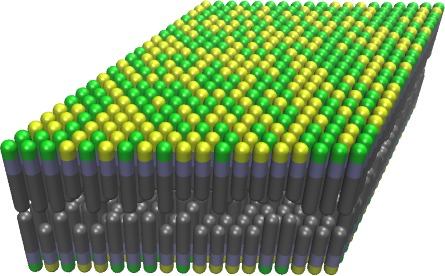
\includegraphics[width=5cm]{lipid_bilayer_mixture.jpg}
\hspace{0.5cm}
\textbf{b)}
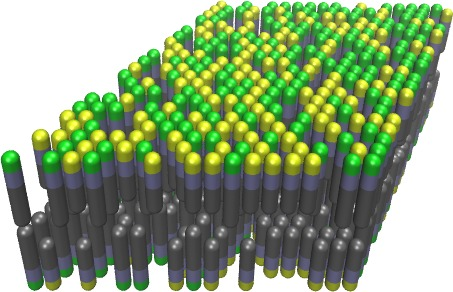
\includegraphics[width=5cm]{lipid_bilayer_vacancies.jpg}
%\newline
%\vspace{10 mm}
%\newline
\caption{
\label{fig:random_bilayer}
A lipid bilayer membrane composed of a random equal mixture of
two different lipid types in a 1:1 ratio.
(See section \ref{sec:random_advanced}.)
In \textbf{b)} one of the molecule types was left blank
leaving vacancies behind.  
(See section \ref{sec:random_vacancies}.)
}
\end{figure}
\subsection{Inserting random vacancies}
\label{sec:random_vacancies}
The list of molecule types passed to the \mbox{\textit{random()}} function
may contain blanks.  In the next example, 30\% of the lipids are missing:
\begin{verbatim}
lipids = new random([DPPC, ,DLPC], [0.35,0.3,0.35], 123) # 2nd element is blank
                    [19].move(7.5,    0,     0)
                    [22].move(3.75, 6.49519, 0)
                     [2].rot(180, 1, 0, 0)     
\end{verbatim}
The results are shown in figure \ref{fig:random_bilayer}b).
\textit{(Note: When this happens, the array will contain missing elements.
 Any attempt to access the atoms inside these missing molecules will
 generate an error message, 
 however moving or deleting array entries 
 using [*] or [i-j] notation should be safe.)}

\subsubsection{Random multidimensional arrays with exact type counts}
\label{sec:random_multidim_exact}
Due to random fluctuations the number of DPPC and DLPC lipids created 
may not equal exactly 0.35 $\times$ of the number of entries in the array,

Alternately, you can specify the exact number of DPPC and DLPC molecules
you desire (as opposed to a list of probabilities).
To do this, replace the list of probabilities with integers:
\begin{verbatim}
lipids = new random([DPPC, ,DLPC], [293,250,293], 123)
                    [19].move(7.5,    0,     0)
                    [22].move(3.75, 6.49519, 0)
                     [2].rot(180, 1, 0, 0)     
\end{verbatim}
This will generate exactly 293 DPPC and DLPC molecules
(and 250 \textit{blank} entries, 
since the second molecule type was unspecified).
The sum (ie 293+250+293) must equal the number of entries in the 
array you are creating (ie 19x22x2).

\subsection{Cutting rectangular holes using \textbf{delete}}
\label{sec:delete_holes}
The delete command can be used to cut large holes in 
1, 2, and 3-dimensional objects.
For example, consider a simple 3-dimensional 12x12x12 cube of molecules.
(For simplicity, each ``molecule'' in this example contains only one atom.
 These atoms appear as blue spheres in figure \ref{fig:delete_holes}.)
\begin{verbatim}
molecules = new OneAtomMolecule [12].move(3.0,0,0)
                                [12].move(0,3.0,0)
                                [12].move(0,0,3.0)
\end{verbatim}
Then, we cut out some rectangular vacancies:
  %The first two commands below delete two layers of molecules 
  %near the top and bottom of the cube.
  %The last command deletes a rectangular box of molecules near the center.
\begin{verbatim}
delete molecules[*][*][2]      
delete molecules[*][*][8]      
delete molecules[6-7][0-8][5-6]
\end{verbatim}
The result of these operations is shown in figure
\ref{fig:delete_holes}.
\textit{(Note: You may move or delete previously deleted array elements
         more than once, and/or deleting overlapping rectangular regions
         without error.)}

\begin{figure}[htbp]
\centering
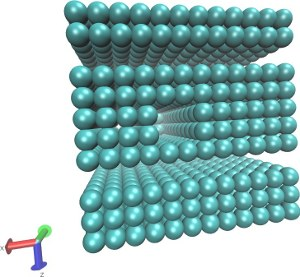
\includegraphics[width=4.0cm]{delete_holes1.jpg}
\caption{
\label{fig:delete_holes}
Rectangular holes can be carved out of an array of molecules
(represented here by blue spheres)
using the ``delete'' command.  Three delete commands were used to
remove the two planar regions and the rectangular hole in the center.
}
\end{figure}






\section{Customizing molecule position and topology}
\label{sec:custom_xform}
By default, each copy of a molecule created using the \textit{new}
command is identical.  This need not be the case.

As discussed in section \ref{sec:xform_after_instance},
individual molecules which were recently created
can be moved, rotated, and scaled.
You can also overwrite or delete individual atoms, 
bonds, and other interactions within a molecule, or their subunits.
(See sections 
\ref{sec:delete_atoms_bonds}, 
\ref{sec:custom_atom},
\ref{sec:custom_bond},
and \ref{sec:adding_atoms_bonds}.)
You make any of these modifications to \textit{some} copies 
of the molecule without effecting other copies.
Furthermore, if those molecules are compound objects 
(if they contain individual molecular subunits within them),
then you can rearrange the positions of their subunits as well.
And all of this can be done from anywhere else in the LT file.
  %\textit{(The notation in section \ref{sec:paths} explains
  %         how to navigate the object hierarchy.)}

For example, suppose we used the ``Polymer'' molecule we defined above
to create a larger, more complicated ``MolecularComplex'' molecule.
\begin{verbatim}
MolecularComplex inherits ForceField {
  polymers[0] = new Polymer
  polymers[1] = new Polymer.rot(180,1,0,0).move(0, 12.4, 0)
}
mol_complex = new MolecularComplex
\end{verbatim}
The \textit{MolecularComplex} molecule is shown in figure \ref{fig:mol_complex}a). 
\textit{Optional: If you want all the atoms in a ``MolecularComplex'' to share the same molecule-ID,
then define ``MolecularComplex'' this way:}
\begin{verbatim}
MolecularComplex inherits ForceField {
  create_var { $mol }
  polymers[0] = new Polymer
  polymers[1] = new Polymer.rot(180,1,0,0).move(0, 12.4, 0)
}
\end{verbatim}
\textit{For this to work, you must also delete the 
 \mbox{\textit{``create\_var \{\$mol:.\}''}} line from
 the definition of the Polymer molecule. See section \ref{sec:2bead}.}


We can subsquently customize the position of the 3rd monomer (``monomers[2]'')
of the second polymer (``polymers[1]''), this way:
\begin{verbatim}
mol_complex/polymers[1]/monomers[2].move(0,0.2,0.6)
\end{verbatim}

This does not effect the position of
\textit{monomers[2]} in \textit{polymers[0]}.
(or in any other \textit{``Polymer''} or
\textit{``MolecularComplex''} molecule.)
If you want to do the same thing for both polymers,
you could use a wildcard character ``*''
\begin{verbatim}
mol_complex/polymers[*]/monomers[2].move(0,0.2,0.6)
\end{verbatim}
If you want to move both polymers, you can use:
\begin{verbatim}
mol_complex/polymers[*].move(0,0.2,0.6)
\end{verbatim}
you could use a wildcard character ``*''
(You can also use ranged (slice) notation, such as ``polymers[0-1]'',
 as an alternative to ``polymers[*]''. 
See section \ref{sec:array_wildcards_intro}.

To make changes that apply to every subsequently created \textit{``Polymer''}
or \textit{``MolecularComplex''} molecule,
see section \ref{sec:molecule_customization}.)


\subsection{Customizing individual atoms or bonds}

\subsubsection{Customizing individual atom locations}
\label{sec:custom_atom}
The ``move'' or ``rot'' commands can not be used to control the positions
of \textit{individual atoms}.
Instead simply overwrite their coordinates this way:
%$atom:mol_complex/polymers[0]/monomers[2]/CA $mol:mol_complex/polymers[1] @atom:R 0 6.4 8.0 0
\begin{verbatim}
write("Data Atoms") {
  $atom:mol_complex/polymers[0]/monomers[2]/ca $mol:mol_complex @atom:R 0 6.4 8.2 0.6
}
\end{verbatim}
This is an case where we must use the \textit{full} variable name of the atom
(``\$atom:mol\_complex/polymers[0]/monomers[2]/ca'')
to indicate \textit{which} ``ca'' atom we want to overwrite
(In this case, we want to modify the ``ca'' atom belonging to
 ``monomers[2]'' in ``polymers[0]'' in ``mol\_complex'').

\subsubsection{Customizing individual bonds, angles, dihedrals,...}
\label{sec:custom_bond}
Similarly, you can customize existing bonds, angles, etc... by overwriting the
line containing a reference to that particular bond (or angle, ...).
For example, you can increase the rest length of the spring representing
the 3rd backbone bond in the first polymer, 
by changing it from type ``@bond:Backbone'' to ``@bond:LongBond''
\begin{verbatim}
write("Data Bonds") {
  $bond:mol_complex/polymers[0]/backbone3 @bond:ForceField/LongBond &
      $atom:mol_complex/polymers[0]/monomers[2]/ca &
      $atom:mol_complex/polymers[0]/monomers[3]/ca 
}
\end{verbatim}
Note: The optional ``\&'' character is used in LAMMPS to split a long command
into multiple lines.
This command is quite long since we are outside the definition
of the polymer molecule, and we must provide the full-path for every variable
(for example ``mol\_complex/polymers[0]'', and ``ForceField'').

Alternatively, if you prefer, you can \textit{delete} the bond 
and define a new bond connecting the same pair of atoms
(see section \ref{sec:delete}).

Of course, at some point you must also create a new ``bond\_coeff''
command defining the properties of this new type of bond
(for example to increase the length of the new spring).
You can either edit the ``forcefield.lt'' file,
\textit{or} simply add the following lines
of text somewhere in one of your .LT files (for example ``system.lt'')
\begin{verbatim}
# Note: This will augment the "ForceField" object, not overwrite it:
ForceField { 
  write_once("In Settings") {
    #             new bond-type   k    r0
    bond_coeff  @bond:LongBond   10.0  4.8
  }
}
\end{verbatim}



\subsection{Adding bonds and angles to individual molecules}
\label{sec:adding_atoms_bonds}
Adding additional bonds within a molecule can be accomplished
by writing additional lines of text to the ``Data Bonds'' section.
(This is what we did when we added bonds between monomers to create a polymer
 in section \ref{sec:2beadPolymer}.)
Again, bonds and atom names must be referred to by their \textit{full} names.
Bonds and bonded interactions can be deleted using the ``delete'' command.
(See section \ref{sec:delete}.)


\subsection{The \textbf{delete} command}
\label{sec:delete}

\subsubsection{Deleting molecules or molecular subunits}
Molecules can be further customized by deleting 
individual atoms, bonds, bonded-interactions, and entire subunits.
We can \textbf{delete} the 3rd monomer of the second polymer, 
use the ``delete'' command:
\begin{verbatim}
delete mol_complex/polymers[1]/monomers[2]
\end{verbatim}

\subsubsection{Deleting atoms, bonds, angles, dihedrals, and impropers}
\label{sec:delete_atoms_bonds}
Individual atoms or bonds can be deleted in a similar way:
\begin{verbatim}
delete mol_complex/polymers[1]/monomers[3]/ca   #<-- deletes the "ca" atom
delete mol_complex/polymers[1]/monomers[4]/cr   #<-- deletes the "cr" bond
\end{verbatim}
Whenever an atom or a molecule is deleted, the bonds, angles, dihedrals, 
and improper interactions involving those atoms are deleted as well.
\textit{Note: You must omit the ``\$'' character when deleting atoms,
bonds, or angles, as we did in the two lines above).}


  %\textit{(In fact, any lines of text in any ``write()'' statement 
  %containing references to deleted atoms are omitted.

When a bond is deleted, any angular, dihedral, or improper 
interactions which were \textit{automatically} 
generated by moltemplate are removed as well.
(However other bonded interactions explicitly listed by the user in their
``Data Angles'', ``Data Dihedrals'', or ``Data Impropers'' sections
are not removed.  These need to be deleted manually.)

Multiple molecules can moved or deleted in a single command.  For example,
the following command deletes the third, fourth, and fifth monomers from 
both polymers[0] and polymers[1]:
\begin{verbatim}
delete mol_complex/polymers[*]/monomers[2-4]
\end{verbatim}
See section \ref{sec:array_wildcards_intro} for an
explanation of ranged (``[2-4]'') array notation, 
and wildcard characters (``*'').

\textit{Minor bug notice: 
Deleting atoms or molecules may cause 
inaccuracies in the \$atoms, \$bonds, \$angles, \$dihedrals, and \$impropers
sections of the ``ttree\_assignments.txt'' file.
(If this is a problem, please email me. -Andrew 2019-9-03.)
Fortunately, this should not harm the resulting LAMMPS data files or input
scripts generated by moltemplate.  They should still work with LAMMPS.}

\textit{WARNING: The \textbf{delete} feature is experimental.
There have been a few bugs in the \textbf{delete} command, but by 2019-9-03
these should be fixed.  Please report any problems you find.
As always, be sure to visualize your structures 
to make sure they look reasonable.
(...by running moltemplate.sh using the 
 ``-vmd'' command line option, for example.
 See sections \ref{sec:vmd_topotools}, \ref{sec:vmd_advanced} for details.)}
%\textit{\textbf{BUG Warning:}
%As of 2019-9-03, delete does not always work 
%when the deleted molecule is both bonded to other molecules,
%and when it contains sub-molecules of it's own.
%The temporary work-around is simply to avoid connecting bonds to any molecule
%which you plan to delete later.  I plan to fix this bug eventually.
%}



  %\subsubsection*{The context() modifier.}
  %\textit{THIS FEATURE DOES NOT WORK YET AS OF 2019-9-03}
  %By default, this transformations is applied relative
  %to the coordinate system in which the command was given.
  %In other words, this command will move the third 
  %monomer of polymers[1] in the +Y direction 
  %regardless of the direction that the molecule ``monomers[2]'' is facing.
  %Alternately, if we want to apply this transformation 
  %in polymers[1]'s local coordinate system, 
  %we would use the context(polymers[1]) command:
  %\begin{verbatim}
  %mol_complex/polymers[1]/monomers[2].context(polymers[1]).move(0,1,0)
  %\end{verbatim}


%\subsubsection*{Examples using center-of-mass coordinate transformations}
%\textit{WARNING: experimental feature 2019-9-03}
%
%You can also center a molecule around it's center-of-mass using ``movecm()'',
%rotate it, and then move it this way:
%\begin{verbatim}
%re6s = new Monomer.movecm(0,0,0).rot(180.0, 1,0,0).move(14.2, 0, 0)
%\end{verbatim}
%By default all rotations are about the origin, not the center-of-mass.
%You can also rotate a molecule around it's center-of-mass using ``rotcm()''
%(without centering it first), and them move the molecule this way:
%\begin{verbatim}
%res6 = new Monomer.rotcm(180.0, 1,0,0).move(14.2, 0, 0)
%\end{verbatim}


\subsection{Customizing molecule \textit{types}}
\label{sec:molecule_customization}
You can create modified versions of existing molecule \textit{types}, 
without having to redefine the entire molecule. For example:
\begin{verbatim}
MolecularComplex0 = MolecularComplex.move(-9.6,-6.2, 0).scale(0.3125)
\end{verbatim}
or equivalently:
\begin{verbatim}
MolecularComplex0 = MolecularComplex
MolecularComplex0.move(-9.6,-6.2, 0).scale(0.3125)
\end{verbatim}
This creates a new type of molecule named ``MolecularComplex0'' whose 
coordinates have been centered and rescaled.
(Note that the ``scale()'' command only effects the atomic coordinates.
(You will have to override earlier force field settings,
such as atomic radii and bond-lengths in order for this to work properly.)
If we want to make additional customizations
(such as adding atoms, bonds, or molecular subunits), we could use this syntax:
\begin{verbatim}
MolecularComplex0 = MolecularComplex

# Add some new atoms connecting the two polymers in the mol_complex

MolecularComplex0 inherits ForceField {
  write("Data Atoms") {
    $atom:t1 $mol:. @atom:CA   0.0   23.0   0.0     0.0
    $atom:t2 $mol:. @atom:CA   0.0   24.7   4.0     0.0
    $atom:t3 $mol:. @atom:CA   0.0   24.7   8.4     0.0
    $atom:t4 $mol:. @atom:CA   0.0   23.0   12.4    0.0
  }
  write("Data Bonds") {
    $bond:b1 @bond:Backbone $atom:polymers[0]/res7/CA $atom:t1
    $bond:b2 @bond:Backbone $atom:t1 $atom:t2
    $bond:b3 @bond:Backbone $atom:t2 $atom:t3
    $bond:b4 @bond:Backbone $atom:t3 $atom:t4
    $bond:b5 @bond:Backbone $atom:t4 $atom:polymers[1]/res7/ca
  }
}

# Center and rescale the atoms in all "MolecularComplex0"
MolecularComplex0.move(-9.6,-6.2, 0).scale(0.3125)
\end{verbatim}
The result of these modifications is shown in figure \ref{fig:mol_complex}b).
\begin{figure}[htbp]
\centering
\textbf{a)}
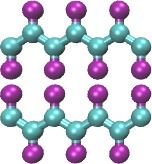
\includegraphics[height=3cm]{mol_complex_LR.jpg}
\hspace{1cm}
\textbf{b)}
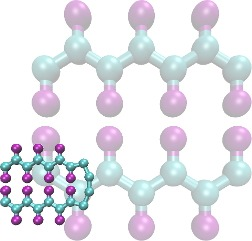
\includegraphics[height=3cm]{mol_complex+mol_complex0_transparent_LR.jpg}
%\newline
%\vspace{10 mm}
%\newline
\caption{
\label{fig:mol_complex}
\textbf{a)}
The ``MolecularComplex'' molecule.  This is a contrived example consisting of
two ``Polymers''.  See section \ref{sec:2beadPolymer}
\textbf{b)}
A customized version of the ``MolecularComplex'' molecule.  
(The original ``MolecularComplex'' is shown faded in the background for comparison.)
}
\end{figure}


\textit{Note: These coordinate transformations will be 
applied \textbf{after} the molecule is constructed.
(If you add atoms to the molecule, these will be added before
the coordinate transformations are applied,
even if you issue the command later.)
Consequently, to make things clear, 
I recommend placing the coordinate transforms applied to 
an entire molecule type \textbf{after} all of its internal details 
(bonds, atoms, subunits) have been declared, as we did here.}

\subsubsection*{\textit{(Advanced)} Inheritance}
\label{sec:inheritance_intro}
The \textit{MolecularComplex0} molecule is a type of \textit{MolecularComplex} molecule.
For those who are familiar with programming, 
relationships like this are analogous to the relationship 
between parent and child objects in an object-oriented programming language.
  %What we have done is equivalent to saying that
  %\textit{MolecularComplex0} inherits from \textit{MolecularComplex}.
More general kinds of inheritance are supported by moltemplate
and are discussed in section \ref{sec:inheritance}.

\subsubsection*{\textit{(Advanced)} Multiple Inheritance}
If we wanted, we could have created a new molecule type 
(like \textit{``MolecularComplex0''}) 
which includes atom types and features from 
\textit{multiple} different types of molecules.
Section \ref{sec:inheritance} mentions one way to do this
and section \ref{sec:inheritance_vs_object_composition}
discusses alternate approaches.








\section*{Advanced moltemplate usage}



\section{Portability: Using \textit{LT files} for force-field storage}
\label{sec:spce_example_robust}
The ``.LT'' format is a flexible file format
for storing force field parameters in LAMMPS.
If you want to share your ``.LT'' file with others, it's 
not safe to assume that all interactions use the same standard formula.

\subsection{Mixing molecule types}
LAMMPS has the ability to combine molecules using multiple different 
force-field styles together using. 
  %Atoms of one type may interact with 
  %each other using inexpensive Lennard-Jones potentials. 
  %Other atoms in the same simulation 
  %may interact using tabulated potentials, 
  %orientation-dependent ellipsoidal potentials, 
  %or even more complex 3-body forces (for example). 
  %Each of these different force-fields is calculated 
  %using code from different source files. 
  %LAMMPS is popular among users who add 
  %their own custom source files.
In section \ref{sec:spce_example}, 
we provided an example of an SPCE water molecule model.
This example was simple to understand.
However, as written, it would be impossible to combine this definition of water 
with other molecules which don't share the same simple bond or angle styles.
For example, we used harmonic restoring forces to preserve the water angle 
at $109.47^\circ$, but other users may want to mix this SPCE water with a small 
number of molecules which use a more complicated angular potential formula,
or tabular angle potentials.
Using the ``hybrid'' keyword, you can avoid this limitation. 
   %being limited to one particular 
   %formula to describe all of the bonds, angles, dihedrals
   %(and pair and improper) interactions.
A more robust example is included below.

\begin{verbatim}
# file "spce.lt" 
#
#    H1     H2
#      \   /
#        O

SPCE {

  write_once("In Init") {
    # -- Default styles (for solo "SPCE" water) --
    units        real
    atom_style   full
    pair_style   hybrid lj/charmm/coul/long 9.0 10.0 10.0
    bond_style   hybrid harmonic
    angle_style  hybrid harmonic
    kspace_style pppm 0.0001
    pair_modify  mix arithmetic
  }

  # AtomID  MolID("."=this)  AtomType  charge  coordX   coordY   coordZ
  write("Data Atoms") {
    $atom:O  $mol:. @atom:O -0.8476  0.0000000 0.00000 0.000000
    $atom:H1 $mol:. @atom:H  0.4238  0.8164904 0.00000  0.5773590
    $atom:H2 $mol:. @atom:H  0.4238  -0.8164904 0.00000 0.5773590
  }

  # atom-type  Mass
  write_once("Data Masses") {
    @atom:O    15.9994
    @atom:H     1.008
  }

  # -- Forces between atoms (non-bonded) --

  #           atomTypeI atomTypeJ    pair-style-name    parameter-list
  write("In Settings") {
    pair_coeff   @atom:O @atom:O  lj/charmm/coul/long   0.1553  3.166 
    pair_coeff   @atom:H @atom:H  lj/charmm/coul/long   0.0     2.058
  }

  # -- Forces between atoms (bonded) --

  #  bond-id   bond-type  atom-id1 atom-id2
  write("Data Bonds") {
    $bond:oh1  @bond:OH   $atom:O  $atom:H1
    $bond:oh2  @bond:OH   $atom:O  $atom:H2
  }

  #             bond-type   bond-style-name  parameter-list
  write("In Settings") {
    bond_coeff   @bond:OH      harmonic      200.0   1.0 
  }

  # angle-id   angle-type  atom-id1 atom-id2 atom-id3
  write("Data Angles") {
    $angle:hoh @angle:HOH  $atom:H1 $atom:O $atom:H2
  }

  #              angle-type  angle-style-name  parameter-list
  write("In Settings) {
    angle_coeff  @angle:HOH    harmonic        200.0   109.47
  }

  # miscellaneous
  write_once("In Settings") {
    group spce type  @atom:O  @atom:H
    fix fSHAKE spce shake 0.0001 10 100 b @bond:OH a @angle:HOH
    # (Remember to "unfix" fSHAKE during minimization.)
  }

} # SPCE
\end{verbatim}
There are two differences between this molecule definition
and the ``spce\_simple.lt'' example from section
\ref{sec:spce_example}:

\subsubsection*{Hybrid force field styles}
  %Each one of these ``\_style'' commands above contains the 
  %``hybrid'' keyword, and followed by a single force-field style
  %(such as ``harmonic'', or ``lj/charmm/coul/long''). 
To experienced LAMMPS users, it may seem strange 
that in this example that we have chosen ``hybrid'' 
styles followed by only one force-field style (``harmonic'').
    %This is due to a quirk in the way LAMMPS reads input script files:
    %We do this so that we later have the option to customize 
    %the force field style for every 
    %pair\_coeff, 
    %bond\_coeff, 
    %angle\_coeff, 
    %dihedral\_coeff, 
    %and improper\_coeff command.  
  %This syntax is only allowed when using ``hybrid'' styles.
  %It's nice to have the option to be able to 
  %customize force-field style after every interaction.
  %Again, we don't need to do that if we are only simulating water,
  %it might be necessary if we are combining SPCE water with other
  %molecule types which use different styles.
However this will make your molecule easier to share with others. 
When other people use your LT file, they can override these
styles as explained in section \ref{sec:overriding_styles}.

%\subsection{Include a default style:}
%LAMMPS requires users to include 
%``atom\_style'',``bond\_style'', ``angle\_style'' 
%commands in the ``Init'' section 
%(which is part of the LAMMPS input script).
%We did this at the beginning of the definition of the ``SPCE'' molecule. 
%The bond and angle styles may clash with the force-field styles 
%used by other molecules we might want to interact with. 
%Presumably the final list of styles will be specified later on by the users 
%who include our ``spce.lt'' molecular file into their simulations,
%overriding our settings.
%However it's always a good idea to provide a list of \textit{default styles} 
%just in case they don't. 

%\subsubsection*{Splitting molecule definitions into multiple files.}
%Alternately, we could eliminate the ``In Init'' section from our
%``spce.lt'' file and create another LT file containing the following
%additional text:
%   %# -- All settings below are optional and can be overridden later.--
%\begin{verbatim}
%# file "spce_defaultstyles.lt"
%SPCE { # <-- Append additional content to the "SPCE" molecule
%  write_once("In Init") {
%    # -- Default styles (for solo "SPCE" water) --
%    units        real
%    atom_style   full
%    pair_style   hybrid lj/charmm/coul/long 9.0 10.0 10.0
%    bond_style   hybrid harmonic
%    angle_style  hybrid harmonic
%    kspace_style pppm 0.0001
%    pair_modify  mix arithmetic
%  }
%}
%\end{verbatim}
%\textit{
%(Note that additional ``SPCE \{...\}'' wrapper
%merely appends additional content 
%to the ``SPCE'' molecule defined in ``spce.lt''.
%This does not overwrite SPCE.)
%}
%Splitting up a molecule into multiple files is usually 
%not necessary, especially for small molecules.


  %(We note that it is necessary to include the ``hybrid'' keyword in the
  %``pair\_style'' and ``bond\_style'' commands because this changes the syntax 
  %of the ``pair\_coeffs'', ``bond\_coeffs'', and other ``coeffs'' commands.)



\subsection{Combining molecules with different force field styles}
\label{sec:overriding_styles}
\textit{Later on}, if a user wants to combine the SPCE water molecule
with another molecule which uses a tabular pair\_style (for example), 
they would have to specify the complete hybrid pair\_style in the 
``Init'' section of their LT file.  For example:
\begin{verbatim}
import "spce.lt"
import "other_molecule.lt"

write_once("In Init") {
  pair_style hybrid lj/charmm/coul/long 9 10 10 table spline 1000
}
\end{verbatim}
Note: By placing the ``write\_once("In Init")\{ \}'' statement 
\textit{after} ``import "spce.lt"'', this insures that
the pair\_style commands issued here will override the 
pair\_style commands issued earlier ``spce.lt''.
%  bond_style hybrid harmonic nonlinear
%  angle_style hybrid harmonic cosine/periodic
This allows moltemplate users users to combine their molecules
``spce.lt'' file shown here
with other template files without modification
(assuming the atom styles match).


\subsubsection*{Warning: Force-field parameters belong in ``In Settings'', not ``Data''}

LAMMPS allows users to store force-field parameters (``Coeffs'') in two places:
a DATA file, \textit{or} an INPUT script. 
Similarly, moltemplate technicaly allows you to store these parameters in 
in the ``Data'' sections of your .LT file:
\begin{list}{}
\item write\_once("Data Pair Coeffs")
\item write\_once("Data Bond Coeffs")
\item write\_once("Data Angle Coeffs")
\item write\_once("Data Dihedral Coeffs")
\item write\_once("Data Improper Coeffs")
\item
\end{list}

\textit{However, for portability reasons, this is discouraged.} 
Instead, declare your force field parameters 
as we do in this manual, 
using the corresponding input script commands.
(For example, ``pair\_coeff'', ``bond\_coeff'', ``angle\_coeff'',
 ``dihedral\_coeff'', and ``improper\_coeff''.
As in the examples, all of these commands belong in the 
``write\_once("In Settings")'' sections of your .LT files.)


\subsection{Nesting}
\label{sec:nesting}
Molecule names such as ``Solvent'' (or even ``Water'')
are short and easy to type, but are vague and are not portable.
If you use common, generic molecule names, you will not be able
to combine your molecule templates with templates written 
by others (without carefully checking for naming conflicts).
LT files were meant to be used for storing 
and exchanging libraries of different molecule types.

Suppose, for example, that you want to run a simulation consisting of
different molecule types, each of which belong to different LT files.
Suppose two of the LT files both happen to contain definitions for
``Water''.
Moltemplate does not detect these name clashes automatically 
and instead attempts to merge the two versions of ``Water'' together,
(most likely creating a molecule with 6 atoms instead of 3).
This is presumably not what you want.

As the number of molecule types grows, 
the possibility of naming clashes increases. 
As the behavior of the same molecule can be approximated 
using many different force fields, 
one has to be careful to avoid clashing molecule names.

To alleviate the problem, you can ``nest'' your 
molecules inside the definition of other molecules or 
namespace objects.
This reduces the scope in which your molecule is defined.
See section \ref{sec:butane} for an example.


\subsection{A simple force-field example}
\label{sec:force_field_example_trappe}
Force-field parameters can be shared by groups of related molecules.
In the example below, we create an object named ``TraPPE''.
Later we use it to define a new molecule named ``Cyclopentane''.

The following example defines a coarse-grained (united-atom)
version of a ``cyclopentane'' molecule. (Hydrogen atoms have been omitted.)
In this example, only the atom types (and positions) and the bonds 
connecting them need to be specified.  
The interactions between them are determined automatically 
by the settings in the force-field file ``trappe1998.lt''.
\begin{verbatim}
import "trappe1998.lt"

cyclopentane {

  # AtomID  MolID('.'=this) AtomType  charge coordX  coordY   coordZ
  write("Data Atoms") {
    $atom:c1 $mol:. @atom:TraPPE/CH2 0.0 0.0000 0.000000000 1.0000000
    $atom:c2 $mol:. @atom:TraPPE/CH2 0.0 0.0000 0.951056516 0.3090170
    $atom:c3 $mol:. @atom:TraPPE/CH2 0.0 0.0000 0.587785252 -0.809017
    $atom:c4 $mol:. @atom:TraPPE/CH2 0.0 0.0000 -0.587785252 -0.809017
    $atom:c5 $mol:. @atom:TraPPE/CH2 0.0 0.0000 -0.951056516 0.3090170
  }

  write("Data Bonds") {
    $bond:bond1 @bond:TraPPE/CC $atom:c1 $atom:c2
    $bond:bond2 @bond:TraPPE/CC $atom:c2 $atom:c3
    $bond:bond3 @bond:TraPPE/CC $atom:c3 $atom:c4
    $bond:bond4 @bond:TraPPE/CC $atom:c4 $atom:c5
    $bond:bond5 @bond:TraPPE/CC $atom:c5 $atom:c1
  }
}
\end{verbatim}
(The ``TraPPE/'' is explained below.)
We can create copies of this molecule in the same way we did with SPCE:
\begin{verbatim}
# A cubic lattice of 125 cyclopentane molecules (12-angstrom spacing)
mols = new Cyclopentane [5].move(0,0,12) [5].move(0,12,0) [5].move(12,0,0)
\end{verbatim}
Unlike the SPCE example, we don't have to specify all of the interactions 
between these atoms because the atom and bond types (CH2, CC).
match the type-names defined in the ``trappe1998.lt'' file.
This file contains a collection of atom types and
force-field parameters for coarse-grained hydrocarbon chains.
(See \cite{TraPPE} for details.)
This way, the ``CH2'' atoms in cyclopentane will interact with, 
and behave identically to any ``CH2'' atom from any other molecule 
which uses the TraPPE force field.
(The same is true for other atom types, and interaction-types 
 which are specific to ``TraPPE'', such as
``@atom:TraPPE/CH3'', ``@bond:TraPPE/CC'', etc...
  %\textit{Note:} By default, all variables are \textit{local} variables.
Another molecule which uses the TraPPE force field is discussed 
later in section \ref{sec:butane}.)
The important parts of the ``trappe1998.lt'' file are shown below:
\subsubsection{Namespace example}
\label{sec:trappe}
\begin{verbatim}
# -- file "trappe1998.lt" --

TraPPE {
  write_once("Data Masses") {
    @atom:CH2 14.1707
    @atom:CH3 15.2507
  }
  write_once("In Settings") {
    bond_coeff     @bond:CC      harmonic   120.0   1.54
    angle_coeff    @angle:CCC    harmonic   62.0022 114
    dihedral_coeff @dihedral:CCCC opls 1.411036 -0.271016 3.145034 0.0
    pair_coeff @atom:CH2 @atom:CH2 lj/charmm/coul/charmm 0.091411522 3.95
    pair_coeff @atom:CH3 @atom:CH3 lj/charmm/coul/charmm 0.194746286 3.75
    # (Interactions between different atom types use mixing rules.)
    # (Hybrid styles were used for portability.)
  }
  write_once("Data Angles By Type") {
    @angle:CCC @atom:C* @atom:C* @atom:C* @bond:CC @bond:CC
  }
  write_once("Data Dihedrals By Type") {
   @dihedral:CCCC @atom:C* @atom:C* @atom:C* @atom:C* @bond:CC @bond:CC @bond:CC
  }
}
\end{verbatim}
In addition to the atom-type names and masses, 
this file stores the force-field parameters (coeffs) for the 
interactions between them.

\subsubsection*{Bonded interactions \textit{by type}}
Again, the ``Data Angles By Type'' and ``Data Dihedrals By Type'' sections 
tell moltemplate.sh that bonded 3-body and 4-body interactions exist between
any 3 or 4 consecutively bonded carbon atoms (of type CH2, CH3, or CH4)
assuming they are bonded using ``CC'' (saturated) bonds.
The ``*'' character is a wild-card.
``C*'' matches ``CH2'', ``CH3'', and ``CH4''.
(Bond-types can be omitted or replaced with wild-cards ``@bond:*''.)

%(moltemplate.sh can automatically generate bonded angle, dihedral, and improper
%interactions between bonded atoms according to their \textit{type} 
%as well as bond type connecting them.
%Note: The syntax used in the ``Data Angles By Type'' and ``Data Dihedrals By Type''
%sections is explained in more detail in appendix \ref{sec:nbody_by_type}.
%
%The ability to specify interactions by atom type instead of atom ID hardly
%matters for the simple water molecule example above but it is useful for
%large molecules. However it makes the LT file format useful for storing
%force-field parameters. It allows local interactions to be specified between
%atoms in complicated molecules which have not been defined yet, (based on
%their local connectivity and atom type).



\subsubsection*{Namespaces and nesting:}
Names like ``CH2'' and ``CC'' are extremely common.
To avoid confusing them with similarly named atoms and bonds 
in other molecules, we enclose them (``nest'' them) within a 
\textit{namespace} (``TraPPE'', in this example).
Unlike ``SPCE'' and ``Cyclopentane'', ``TraPPE'' is not a molecule.
It is just a container of atom types, bond-types and 
force-field parameters shared by other molecules.
We do this to distinguish them from other atoms and bonds 
which have the same name, but mean something else.
Elsewhere we can refer to these atom/bond types as
``@atom:TraPPE/CH2'' and ``@bond:TraPPE/CC''.
(You can also avoid repeating the cumbersome ``TraPPE/'' prefix 
 for molecules defined within the TraPPE namespace.
 For example, see section \ref{sec:butane}.)





\subsection{Nested molecules}
\label{sec:butane}
Earlier in section \ref{sec:trappe}, we created an object named ``TraPPE''
and used it to create a molecule named ``Cyclopentane''.
Here we use it to demonstrate nesting.
Suppose we define a new molecule ``Butane'' consisting of 4 coarse-grained
(united-atom) carbon-like beads, whose types are named ``CH2'' and ``CH3''.
\begin{verbatim}
# -- file "trappe_butane.lt" --

import "trappe1998.lt"

Butane {
  write("Data Atoms"){
    $atom:c1 $mol:. @atom:TraPPE/CH3 0.0  0.419372  0.000 -1.937329
    $atom:c2 $mol:. @atom:TraPPE/CH2 0.0  -0.419372  0.000 -0.645776
    $atom:c3 $mol:. @atom:TraPPE/CH2 0.0  0.419372  0.000  0.645776
    $atom:c4 $mol:. @atom:TraPPE/CH3 0.0  -0.419372  0.0000 1.937329
  }
  write("Data Bonds"){
    $bond:b1 @bond:TraPPE/CC $atom:c1 $atom:c2
    $bond:b2 @bond:TraPPE/CC $atom:c2 $atom:c3
    $bond:b3 @bond:TraPPE/CC $atom:c3 $atom:c4
  }
}
\end{verbatim}
  %Note that we inserted ``../TraPPE/'' prefix before ``CH2'', for example, 
  %to inform moltemplate/ttree that we want to use the ``CH2'' 
  %atom that defined inside ``../TraPPE''.
  %(This is the same thing we did in section \ref{sec:trappe}.)
  %The ``../'' before ``TraPPE'' is optional.

  %It informs moltemplate.sh that ``TraPPE'' was defined 
  %in the parent's environment (IE, one level up).
  %(Note: If you omit the ``../'', moltemplate will automatically 
  %look for it there in any case, so this is optional.)

Alternately, as mentioned above, it may be simpler to nest our ``Butane'' 
within ``TraPPE'', so that so that it does not get confused with other
(perhaps all-atom) representations of butane.  In that case, we would use:
\begin{verbatim}
# -- file "trappe_butane.lt" --

import "trappe1998.lt"

TraPPE {
  Butane {
    write("Data Atoms"){
      $atom:c1 $mol:. @atom:../CH3 0.0  0.419372  0.000 -1.937329
      $atom:c2 $mol:. @atom:../CH2 0.0  -0.419372  0.000 -0.645776
      $atom:c3 $mol:. @atom:../CH2 0.0  0.419372  0.000  0.645776
      $atom:c4 $mol:. @atom:../CH3 0.0  -0.419372  0.0000 1.937329
    }
    write("Data Bonds"){
      $bond:b1 @bond:../CC $atom:c1 $atom:c2
      $bond:b2 @bond:../CC $atom:c2 $atom:c3
      $bond:b3 @bond:../CC $atom:c3 $atom:c4
    }
  }
}
\end{verbatim}
Note: Wrapping Butane within ``TraPPE\{ \}'' clause merely appends 
additional content to be added to the ``TraPPE'' object defined 
in the ``trappe1998.lt'' file (which was included earlier). 
It does not overwrite it. 
Again ``../'' tells moltemplate use the ``CH2'' atom 
defined in the context of the TraPPE environment (IE. one level up).
This insures that moltemplate does not create a new ``CH2'' atom type
which is local to the Butane molecule.  
(Again, by default all atom types and other variables are local.
See section \ref{sec:variable_scope}.)
  % However moltemplate.sh does check the parent/ancestor environments
  % before creating a new variable, so ``../'' is not strictly necessary
  % in this example.)

To use this butane molecule in a simulation, 
you would import the file containing the butane definition,
and use a ``new'' command to create one or more butane molecules.
\begin{verbatim}
import "trappe_butane.lt"
new butane = TraPPE/Butane
\end{verbatim}
(You don't need to import ``trappe1998.lt'' in this example because
it was imported within ``trappe\_butane.lt''.)
The ``TraPPE/'' prefix before ``Butane'' lets moltemplate/ttree
know that butane was defined \textit{locally} within TraPPE.  

  %Of course, additional molecules can be added to 
  %the existing TraPPE namespace by enclosing them within ``TraPPE\{ \}'',
  %brackets, in addition to ``Butane''.


\textit{Note: An alternative procedure using \textbf{inheritance}
exists which may be a cleaner way to handle these kinds of relationships.
See sections \ref{sec:inheritance} and \ref{sec:multiple_inheritance}.}

\subsection{Path syntax: ``../'', ``.../'', and ``\$mol:.''}
\label{sec:paths}
Generally, multiple slashes (``/'') as well as (``../'') can be
used build a path that indicates the (relative) location 
of any other molecule in the object hierarchy. 
(The ``.'', ``/'' and ``..'' symbols are used here in the same way 
they are used to specify a path in a unix-like file-system.
For example, the ``.'' in ``\$mol:.'' refers to the 
current molecule (instance), in the same way that 
``./'' refers to the current directory.
(Note: \mbox{\textit{``\$mol''}} is shorthand for \mbox{\textit{``\$mol:.''}})

A slash by itself, ``/'', refers to the \textit{global environment}.
This is the outermost environment in which all molecules are defined/created.
  %\textit{
  %(Details: These symbols can be used to navigate 
  %both the hierarchy of defined molecule \textbf{types}, 
  %(when preceded by @), 
  %or the hierarchy of \textbf{instantiated} molecules,
  %(when preceded by \$).)
  %}


\subsubsection{\textit{(Advanced)} Ellipsis notation ``.../''}
\label{sec:ellipsis_type}
If you are using multiple levels of nesting,
and if you don't know (or if you don't want to specify) where
a particular molecule type or atom type (such as ``CH2'') was defined, 
you can refer to it using ``.../CH2'' 
instead of ``../CH2''.
The ``...'' ellipsis syntax searches up the tree of nested 
molecules to find the target (the text following the ``/'' slash).

\subsubsection{\textit{(Advanced)} \$mol:... notation}
\label{sec:ellipsis_mol}
Recall that LAMMPS allows users the option to assign
\textit{molecule-IDs} to each atom.
(In the water example (section \ref{sec:spce_example}), atoms in
each water molecule is assigned to a molecule-ID, denoted ``\$mol:.''.
In that example, the ``.'' was the name of that molecule's ID.)

If you want to build large molecules using smaller pieces as building-blocks
moltemplate has a way to allow all the the atoms to share the same molecule-ID.
To refer to the ID of the molecule to which you belong,
use ``\$mol:...''.  (If none of the molecule-objects which 
instantiate the current molecule-object define a variable in the \$mol category,
then a new local \$mol variable will be created automatically.)
This means that the second column of each line of the ``Data Atoms'' section
should contain ``\$mol:...'' 
(assuming ``atom\_style full'' or ``molecular'' is used).

The ``...'' syntax is explained more formally 
in appendix \ref{sec:adv_variable_syntax}.)




\subsection{\textit{using namespace} syntax}
\label{sec:using_namespaces}

Because the \textit{Butane} molecule was defined within the \textit{TraPPE}
environment, you normally have to indicate this when you refer to it later.
For example, to create a copy of a \textit{Butane} molecule, 
you would normally use:
\begin{verbatim}
import "trappe_butane.lt"

butane = new TraPPE/Butane
\end{verbatim}

However for convenience, you can use the 
\mbox{``\textbf{using namespace}''} declaration 
so that, in the future, you can quickly refer to any 
of the molecule types defined within \textit{TraPPE} directly, 
without having to specify their path.
\begin{verbatim}
import "trappe_butane.lt"

using namespace TraPPE

butane = new Butane
\end{verbatim}
\subsubsection*{This only works for molecule types, not atom types}
Unfortunately, you still \textit{must} always
\textbf{refer to} atom types, bond types, and any other
\textbf{primitive types explicitly} (by their full path).
For example, the second line in the \textit{``Data Atoms''} in the example
below does not refer to the \textit{CH2} atom type defined in \textit{TraPPE}.
(Instead it creates a \textit{new} atom type, 
which is probably not what you want.)
\begin{verbatim}
import "trappe_butane.lt"
using namespace TraPPE
butane = new Butane
write("Data Atoms") {
  $atom:c1 $mol @atom:TraPPE/CH2 0.0   0.41937 0.00 1.9373  # <-- yes
  $atom:c2 $mol @atom:CH2        0.0  -0.41937 0.00 -0.6457 # new atom type?
}
\end{verbatim}
If, for example, you want to leave out the ``TraPPE/'' prefix 
when accessing the atom, bond, and angle types defined in TraPPE,
then instead you can define a new molecule which 
\textit{inherits} from TraPPE. (See section \ref{sec:inheritance}.)

\subsection{Inheritance}
\label{sec:inheritance}
We could have defined \textit{Butane} this way:
\begin{verbatim}
import "trappe1998.lt"

Butane inherits TraPPE {
  write("Data Atoms"){
    $atom:c1 $mol:. @atom:CH3 0.0  0.419372  0.000 -1.937329
    $atom:c2 $mol:. @atom:CH2 0.0  -0.419372  0.000 -0.645776
    $atom:c3 $mol:. @atom:CH2 0.0  0.419372  0.000  0.645776
    $atom:c4 $mol:. @atom:CH3 0.0  -0.419372  0.0000 1.937329
  }
  write("Data Bonds"){
    $bond:b1 @bond:CC $atom:c1 $atom:c2
    $bond:b2 @bond:CC $atom:c2 $atom:c3
    $bond:b3 @bond:CC $atom:c3 $atom:c4
  }
}
\end{verbatim}
A molecule which \textit{inherits} from another molecule (or namespace)
\textit{is} a particular type of that molecule (or namespace).
Defining \textit{Butane} this way allows it to 
access all of molecule types, atom types, and bond types, etc...
defined within \textit{TraPPE} as if they were defined locally.
(I did not have to refer to the CH3 atom types as ``@atom:TraPPE/CH3'',
 for example.)

\subsubsection{Multiple inheritance:}
\label{sec:multiple_inheritance}
A molecule can inherit from multiple parents.
This is one way you can allow the \textit{Butane} molecule
to borrow atom, bond, angle, dihedral, and improper types from
\textit{multiple} different force-field parents:
\begin{verbatim}
import "trappe1998.lt"
import "oplsaa.lt"

Butane inherits TraPPE OPLSAA {
  ...
}
\end{verbatim}
\textit{Details:Moltemplate attempts to resolve duplicate atom types or 
molecule types if they are found in both parents, giving priority to the 
first parent in the list of parents following the ``inherits'' keyword. 
(``TraPPE'' in this example.)
  %Note: This feature has not been rigorously tested as of 2019-9-03.)
}

\subsubsection{Inheritance \textit{vs.} Nesting}
\label{sec:inheritance_vs_nesting}
If two molecules are related to each other this way:
\mbox{\textit{``A \textbf{is a} particular type of B''}},
then consider using inheritance instead of nesting
(or object composition).
In this example (with \textit{Butane} and \textit{TraPPE})
either nesting or inheritance would work.

  Again, one very minor advantage to nesting 
\textit{Butane} inside \textit{TraPPE}, is that it prevents the name
\textit{Butane} from being confused with or conflicting with any other 
versions of the \textit{Butane} molecule defined elsewhere.
(Usually this is not a consideration.)

\subsubsection{Inheritance \textit{vs.} Object Composition}
\label{sec:inheritance_vs_object_composition}
On the other hand, if two molecules are related to each other this way:
\mbox{\textit{``A is \textbf{comprised of} B and C''}},
then you might consider using object composition instead of inheritance.
For example:
\begin{verbatim}
import "B.lt"  # <-- defines the molecule type "B"

import "C.lt"  # <-- defines the molecule type "C"

A {
  b = new B
  c = new C
}
\end{verbatim}





  %\section{Inheritance}
  %\label{sec:inheritance}
  %
  %In this section we show a simple example of inheritance and nesting.
  %
  %\textit{INCOMPLETE DOCUMENTATION}
  %\textit{I will finish this example later...}
  %
  %% \ref{fig:LPN}
  %There's no need to define the tail twice. 
  %Instead use inheritance
  %\begin{verbatim}
  %CGLipid {
  %  # Both DOTAP and DOPC lipids share the same tail.
  %  # In the CGLipid model, the tail is represented by 
  %  # a single linear chain.
  %  write("Data Atoms"){
  %    $atom:c1 $mol:. @atom:C 0.0  0.419372  0.00000 -1.481799
  %    $atom:c2 $mol:. @atom:C 0.0  -0.419372 0.00000 -2.773352
  %    $atom:c3 $mol:. @atom:C 0.0  0.419372  0.00000 -4.064904
  %    $atom:c4 $mol:. @atom:C 0.0  -0.419372 0.00000 -5.356457
  %    $atom:c5 $mol:. @atom:C 0.0  0.419372  0.00000 -6.648010
  %  }
  %  write("Data Bonds"){
  %    $bond:c12 @bond:Tail $atom:c1 $atom:c2
  %    $bond:c23 @bond:Tail $atom:c2 $atom:c3
  %    $bond:c34 @bond:Tail $atom:c3 $atom:c4
  %    $bond:c45 @bond:Tail $atom:c4 $atom:c5
  %  }
  %  write("Data Angles"){
  %  :
  %}
  %\end{verbatim}
  %DOPC and DOTP differ only in the head group (which 
  %has only 1 atom in this coarse-grained version).
  %\begin{verbatim}
  %DOPC inherits CGLipid {
  %  write("Data Atoms"){
  %    $atom:head $mol:. @atom:head 0.0  0.000 0.000 0.000
  %  }
  %  write_once("Data Masses"){
  %    @atom:. 245.0
   % }
   % # Now connect the head to the tail
   % write("Data Bonds"){
  %    $bond:head-tail @bond:Head-Tail $atom:head $atom:c1
  %  }
  %  :
  %}

  %DOTAP inherits CGLipid {
  %  write("Data Atoms"){
  %    $atom:head $mol:. @atom:head 0.0  0.000 0.000 0.000
  %  }
  %  write_once("Data Masses") {
  %    @atom:. 122.0
  %  }
  %  write("Data Bonds"){
  %    $bond:head-tail @bond:Head-Tail $atom:head $atom:c1
  %  }
  %  :
  %}
  %\end{verbatim}
  %
  %\textit{INCOMPLETE DOCUMENTATION}
  %\textit{I will finish this example later...}
  %
  %
  %\begin{verbatim}
  %TubulinA {
  %  ...
  %}
  %TubulinB {
  %  ...
  %}
  %TubulinDimer {
  %  a = new A
  %  b = new B
  %}
  %\end{verbatim}
  %\begin{verbatim}
  %Tubulin {
  %  A {
  %    ...
  %  }
  %  B {
  %    ...
  %  }
  %  Dimer {
  %    a = new A
  %    b = new B
  %  }
  %}
  %\end{verbatim}
  %
  %\textit{INCOMPLETE DOCUMENTATION}
  %\textit{I will finish this example later...}



\section{Known bugs and limitations}
\label{sec:limitations}

Please report any bugs you find by email to 

\includegraphics[height=0.3cm]{author_email.png},
or to the lammps-users mailing list.

\textbf{1)} LAMMPS-style molecule-templates are \textit{not} supported.
The DATA files created by moltemplate are not 
in the correct format to be read by the LAMMPS \textit{molecule} command.
(This is because this command was added after moltemplate was written.)
However the formats are similar, and the relevant information can be extracted
using a text-editor and converted to the other format.
(Using a text-editor and awk, or a spreadsheet program.
For more information on these file formats, 
\url{http://lammps.sandia.gov/doc/read_data.html}
\url{http://lammps.sandia.gov/doc/molecule.html}.)
Again, feel free to contact 
\includegraphics[height=0.3cm]{author_email.png}
to request support for LAMMPS-style molecule templates.


\textbf{2)} \textbf{Moltemplate consumes a large amount of memory (RAM)}

Memory use grows proportional to system size.
As of 2019-9-03, setting up a system of 1000000 atoms using moltemplate 
currently requires between 2.7 and 12 GB of \textit{available} memory. 
(Systems with many bonds and angles consume more memory, 
 as well as systems with a high molecule count.)
   %(This is due to python's excessive memory usage.)
Unfortunately this code was not carefully written to minimize memory usage. 
(In addition, python programs can require more than 10 
times as much memory as similar programs written in C/C++.)
   %\textit{(I wish I had known this earlier.)}

This problem might be alleviated by using other 
python interpreters with a lower memory footprint.
Alternately, it may be necessary to split a large system into pieces, 
run moltemplate on each piece, and combine the resulting data files 
into one large data file later.
    %(Each time, you can use the ``category()'' command to force the
    % \$atom, \$bond, \$angle, \$dihedral, \$improper, and \$mol counters
    % to begin at a number larger than 1, so that the values do not overlap.)
  %A strategy for combining data files together is discussed 
  %in appendix \ref{sec:combining_data_files}.

Also, computers with a moderate amount of RAM can be rented very cheaply.
(For example, see \url{https://cloud.google.com/compute/}.)

\textit{When setting up large simulations with moltemplate,
consider using the \mbox{``ulimit''} command}
to prevent system crashes.
(If you are on a shared computer, ask an administrator to do this.)
If these options are not available,
you can always run a resource monitor (like ``top'') before 
starting moltemplate and kill the process if it's memory usage exceeds 80\%.


\textbf{3)} Limited support for non-point-like atoms:

As of 2019-9-03, only the ``full'', ``angle'', ``atomic'', ``charge'',
``sphere'', ``dipole'', ``ellipsoid'', and ``molecular'' styles
have been tested.  
Other non-point-like atoms like ``tri'', ``line'' 
\textit{should} also work with moltemplate. 
However these objects
are \textit{not rotated correctly} 
by the ``.rot()'' command
(or scaled correctly by the ``.scale()'' command).
More exotic exotic atom styles, such as 
``wavepacket'', ``electron'', ``sphere'' and ``peri''
have not been tested.
In addition, atom\_style \textbf{body} and 
atom\_style \textbf{template} are \textit{not} 
supported.
Feel free to contact 
\includegraphics[height=0.3cm]{author_email.png}
to request support for exotic atom styles.


\textbf{4)} 
When placed at the end of a line, LAMMPS interprets 
\textbf{the ``\&'' character} as a 
request to merge two lines together.
\textit{It is usually safe to use this character inside
moltemplate write() or write\_once() commands.}
However in some rare cases, joining two lines together using 
the ``\&'' character can confuse moltemplate. 
For example, in a lammps input script command, 
(like ``pair\_coeff'' or ``dihedral\_coeff''), 
\textbf{the ``\&'' character should not appear before 
the last ``@'' or ``\$'' variable is referenced.}
Also avoid using the ``\&'' character anywhere in the 
``Data Atoms'', ``Data Bonds'', ``Data Angles'', ``Data Dihedrals'', ``Data Impropers'', ``Data Angles By Type'', ``Data Dihedrals By Type'', and ``Data Impropers By Type''
sections.

\textbf{5)} Triclinic boundary conditions have not been tested:

As of 2019-9-03, support for PDB files with triclinic cells is experimental.
Please let me know if it is not working.

\textbf{6)} Inconsistent support for wildcard characters (``*'' and ``?'') 
\label{sec:wildcard_bug}
   The wildcard character ``*''
   is interpreted differently in different parts of an LT file.
   Wildcard characters work reliably and are used for \textit{string}
   pattern matching when inside
   ``bond\_coeff'', ``angle\_coeff'', ``dihedral\_coeff'', ``improper\_coeff'',
   and most ``pair\_coeff'' commands,
   as well as any of the \textit{``By Type''} sections 
   in an LT file (such as
   \textit{``Data Angles By Type''}, 
   \textit{``Data Dihedrals By Type''}, and 
   \textit{``Data Impropers By Type''}).
   However these wildcard characters \textit{do not}
   within pair\_coeff commands that require \textit{more}
   than 2 atom types as arguments.
   (such as ``pair\_style hbond/dreiding/lj''.
    However manybody pair\_styles which use ``pair\_coeff * *''
    notation work fine.)

   %As of 2019-9-03, wildcard characters (``*'', ``?'') also fail to work inside
   %\textit{``bond\_modify''} commands, and other commands used for running
   %active matter simulations. (Such commands are typically located within the
   %\textit{``write\_once("In Transitions")''} section of an .LT file.)
   %LAMMPS interprets ``*'' characters appearing here as
   %\textit{numeric ranges}, and their behavior depends on the
   %integers which moltemplate assigns to these variables,
   %\textit{not} the \textit{names} of the variables.
   %(See the official documentation for bond\_modify, and bond\_coeff
   % commands to see how ``*'' characters are interpreted.
   %This can lead to unintended side-effects and is discouraged.
   %The ``*'' character can be safely used in array brackets, \textit{[*]}, or in
   %the varios \textit{``\_coeff''} commands and \textit{``By Type''} sections.
   %(See section \ref{sec:array_wildcards_intro} 
   % and appendix \ref{sec:nbody_by_type}.)

\pagebreak



\appendix
\section*{Appendices}

\section{Bonded interactions ``By Type''}
\label{sec:nbody_by_type}

Interactions between atoms in LAMMPS which are not bonded together
(ie ``non-bonded'' or ``pair'' interactions) 
are specified \textit{by atom type}.
\textit{Bonded interactions} in LAMMPS, 
(including 3-body angle, and 4-body dihedral and improper interactions),
are specified by unique \textit{atom ID number}.
(There are typically a large number of angles and bonds in 
a typical molecule, and this information occupies the 
majority of in a typical LAMMPS data file.)

This has changed in moltemplate.sh.  moltemplate.sh contains a 
utility which can generate angles, dihedrals, and impropers
automatically by atom and bond \textit{type}.
(This utility is described in section \ref{sec:nbody_by_type_utility}.)
moltemplate.sh will inspect the network of bonds present in your system, 
detect all 3-body, and 4-body interactions, and determine their type.
(Higher n-body interactions can also be defined by the user.)
Specifying interactions this way can eliminate significant redundancy 
since many atoms share the same type. 

To make use of this feature, you would create a new section named
\mbox{``Data Angles By Type''}, \mbox{``Data Dihedrals By Type''}, 
or \mbox{``Data Impropers By Type''} 
whose syntax mimics the 
\mbox{``Angles''}, \mbox{``Dihedrals''}, and \mbox{``Impropers''} 
sections of a LAMMPS data file.
The syntax is best explained by example:

\begin{verbatim}
write("Data Angles By Type") {
  @angle:XCXgeneral       *      *C*      *
  @angle:CCCgeneral    @atom:C @atom:C @atom:C    *         *
  @angle:CCCsaturated  @atom:C @atom:C @atom:C @bond:SAT @bond:SAT
}
\end{verbatim}

%\begin{list}{}
%\item
The first line will generate a 3-body angle interaction 
(of type \mbox{``@angle:XCXgeneral''})
between any 3 consecutively bonded atoms 
as long as the second atom's type-name contains the letter ``C''.
(Atom and bond type-names can contain wildcard characters *)

%\item
The second line will generate a 3-body interaction 
of type \mbox{``@angle:CCCgeneral''}
between any 3 atoms of type \mbox{``@atom:C''},
regardless of the type of bonds connecting them.
(The last two columns, which are both wildcard characters, *, 
 tell moltemplate.sh to ignore the two bond types.
 Since this is the default behavior 
 these two columns are optional and can be omitted.)

%\item
The third line will generate a 3-body interaction of
type \mbox{``@angle:CCCsaturated''}
between any 3 atoms of type \mbox{``@atom:C''},
if they are connected by bonds of type \mbox{``@bond:SAT''}.
%\end{list}

Note: The 2nd and 3rd lines in this example will generate new interactions 
which may override any angle interactions assigned earlier.

\subsection*{Regular expressions}
Regular-expressions can also be used to match potential atom and bond types.
(To use regular expressions, surround the atom and 
bond types on either side by slashes.  
For example: \mbox{@atom:C[1-5]/}, should match 
\mbox{@atom:C1} through \mbox{@atom:C6}.)
\textit{Note: This feature has not been tested as of 2019-9-03.}

In a similar way, one can define ``Dihedrals By Type'' and 
``Impropers By Type''.


  % I THINK I FIXED THIS LIMITATION 
  % SO I COMMENTED OUT THIS NEXT SECTION:
  % IGNORE ALL COMMENTED OUT TEXT IN THE PARAGRAPHS BELOW
  %In all of these examples, the slash ``/'' following the 
  %@ character is explained below.
  %
  %\subsection*{Nesting: ``By Type'' interactions \textit{require full-path} variable syntax}
  %
  %Consider again the atom type named ``CH2'' defined within the ``trappe1998.lt'' 
  %example from section \ref{sec:nesting}.
  %Every atom and bond type defined in that file was defined 
  %inside the ``TraPPE'' namespace.
  %(That file contains a ``TraPPE {...}'' clause.)
  %Consequently any atom types like ``CH2'' are \textit{nested variables}.
  %It's \textit{full name} is ``@/atom:TraPPE/CH2'', not ``@atom:CH2''.
  %However usually you don't have to refer to it this way.
  %When you are inside the ``TraPPE{...}'' clause, it is sufficient 
  %to refer to this atom using ``@atom:CH2''.
  %
  %However moltemplate.sh uses an external program to automatically generate 
  %interactions by type.
  %This program is not smart enough to understand nested variable syntax.
  %So whenever ``write("Data Angles by Type") {...}'' is nested within 
  %a molecule definition, you must refer to the atom types using the 
  %\textit{full-path} syntax
  %(for example: ``@/atom:TraPPE/CH2'', not ``@atom:CH2'').






\section{Using ltemplify.py to create an \textit{LT file}}
\label{sec:ltemplify}

The ``ltemplify.py'' script is used to convert LAMMPS data files and
input into a single MOLTEMPLATE (``\textbf{LT}'') file.

\textbf{\textit{Typically}}, the LT files generated
by ``ltemplify.py'' contain the definition of a single type of molecule
(or molecular complex) present in the data file.
This way, moltemplate users later on can build complicated simulations using
this molecule as a building block (perhaps along with other molecules).

Users can select the molecule (or molecules) they want
using the ``-mol'', ``-id'', or ``-type'' arguments,
and give the molecule a name using the ``-name'' argument.  (See below.)
The resulting LT file will include all of the information relevant
to that molecule including atom types, charges, coordinates,
bonded interactions, force field parameters, force field styles,
groups, and fixes that are relevant to that molecule.
(Other information will be omitted.)

\subsubsection*{Typical Usage}
\begin{verbatim}
ltemplify.py -name MoleculeName -mol MolID INPUT_SCRIPT DATA_FILE > FILE.lt
\end{verbatim}
...where \textit{MoleculeName} is a string,
\textit{MolID} is an integer,
\textit{INPUT\_SCRIPT} and \textit{DATA\_FILE}
are the names of a LAMMPS input script and a data file
containing the molecule of interest,
and \textit{FILE.lt} is the resulting
MOLTEMPLATE file created by ltemplify.py.
(See section \ref{sec:ltemplify_args_table} for more information.)

\subsubsection*{Note: Tiresome details to follow.}
\subsubsection*{First time readers should probably skip to
the examples in section\ref{sec:ltemplify_examples}.}

\subsubsection*{Required arguments}

``ltemplify.py'' requires only one argument: the name of a LAMMPS data file.
However (as shown in the example above), it also reads LAMMPS input scripts.
\textit{(Note: If LAMMPS input scripts are included, they must appear
\textbf{before} the DATA file in the argument list.  See examples below.)}
``ltemplify.py'' also accepts many arguments to select the atoms belonging
to the molecule of interest and customize the output.

\subsubsection*{LAMMPS input scripts}

In addition to LAMMPS DATA files, users can also supply
one or more LAMMPS input scripts
(typically containing information relevant to that molecule,
such as force field parameters and fixes).
If LAMMPS input scripts are included, they must appear \textit{before}
the DATA file in the argument list. (See examples below.)

\pagebreak

\subsection{ Optional arguments }
\label{sec:ltemplify_args_table}
%\begin{table}
\begin{tabular}[h]{l|p{10cm}}
\textbf{argument} & \textbf{meaning}
\\
\hline
\hline

-name \textit{NAME}  &
Specify the name of the molecule described in the output file.
(The optional ``inherits'' keyword can be used to select a force field.)
\\
\hline

-atomstyle \textit{style}
&
Optional: Force ltemplify.py to use a particular atom\_style.
(Hybrid styles should be surrounded by quotes, eg
\textit{-atomstyle "hybrid full dipole"}.)
%For custom atom styles, you can specify the list of column 
%names manually.  For example:
%\textbf{-atomstyle "molid x y z atomid atomtype mux muy muz"}
%Atom styles should be enclosed in quotes (").
\\
\hline

-columns \textit{"column\_list"}  &
For custom atom\_styles, you can list of column names in the ``Atoms''
section manually.
(For example: \textbf{-columns "molid x y z atomid atomtype mux muy muz"})
\\
\hline

-mol \textit{"molID\_list"}
&
Select the molecule you want to appear in in the resulting LT file.
To select more than one molecule, supply a list of numbers surrounded
by quotes.
\\
\hline

-id \textit{"id\_list"}
&
Select atoms by their atom-IDs.
Use quotes to surround the list of atom ID numbers.
Unselected atoms will be omitted.
\\
\hline

-type \textit{"type\_list"}
&
Select atoms by their types.
Use quotes to surround the list of atom type numbers.
\\
\hline

-datacoeffs
&
Put force field information in the data file, not in an input script.
(By default, force field parameters will be placed in the ``In Settings''
 section which will eventually be written to a LAMMPS input script.)
\\
\hline

-ignore-comments
&
Do not infer atom, bond, angle, dihedral, and improper type names
from comments in the data file.
\\
\hline

-ignore-coeffs
&
Ignore all force field parameters (coeffs).
\\
\hline

-ignore-angles
&
Ignore angles, dihedrals and impropers.  Omit from output file.
(This is useful when using force fields which generate angles, dihedrals, and impropers automatically.)
\\
\hline

-ignore-bond-types
&
Ignore the 2nd column in the "Bonds" section of the LAMMPS data file,
and create a "Bond List" section in the resulting MOLTEMPLATE LT file
which omits the bond types.
(This is useful when using force fields which choose bond type automatically.)
\\
\hline

-ignore-masses
&
Ignore all masses in the data file.  Omit from output file.
(This is useful when using force fields, since they typically contain atomic mass definition.)
\\
\hline

-prepend-atom-type \textit{STR}
&
prepend the string from the \textit{STR} argument to the beginning of
all atom type names.
\\
\hline
\end{tabular}


\subsubsection*{Examples showing argument usage are included
                in section \ref{sec:ltemplify_examples}.}

\pagebreak


\subsubsection*{Default behavior}
\textit{Note that by default
(if the ``-mol'', ``-id'', or ``-type'' arguments are omitted),
``ltemplify.py'' will copy \textbf{all} of the information
from the LAMMPS files into an LT file that describes the entire system.
Normally, this is not very useful.}



\subsubsection*{Details}

All atoms, bonds, angles, dihedrals, and impropers and their associated
types will be converted to moltemplate ``\$'' or ``@'' counter variables
(and the relevant portion of each file will be moved to sections
with the correct header names).
Coefficients, atom styles, and most force-field styles and
settings \textit{should} also be included in the resulting .LT file.
ltemplify.py also understands simple group commands
(using ``id'', ``molecule'', or ``type'' styles)
and ``fix shake'' and ``fix rigid''  (untested 2019-9-03).
However most other fixes, and complex group commands are not understood.
Those commands must be added to the resulting .LT file manually.
(See section \ref{sec:ltemplify_limitations} for more details.)



\subsection{Fixes and Groups}
\label{sec:ltemplify_fix_group}

\textit{ltemplify.py} has
\textit{limited} support for ``fix'' and ``group'' commands,
including ``fix shake'', ``fix rigid'', and ``fix poems''.
Other fixes must be added manually to the file generated by ltemplify.py.
(Such as fix ``restrain'', ``bond/create'', ``bond/break'', ``bond/react'',
 ``ttm'', etc...)

ltemplify.py can understand simple (static) ``group'' commands, and will include them in the output file, if it can determine that they contain any relevant atoms.  (Fixes depending on irrelevant groups are also deleted.)

\textit{Note: This feature has not been tested carefully.  So please review all of the group and fix commands generated by ltemplify.py to make sure they refer to the correct atoms.  And please report any bugs you find. (-Andrew 2019-9-03)}



\subsubsection*{Automatic generation of atom, bond, angle, dihedral, improper names}

By default ltemplify.py generates atom, bond, angle, dihedral, and improper,
type names and id names automatically.
This resultis in atoms with types like ``@atom:type3'', and IDs like
``\$atom:type3\_7'' (I.e. the 7th atom of type 3.)

\subsubsection*{ Inferring atom type names from comments }

\textit{However,} ltemplify.py uses comments in the ``Masses'' section of
the LAMMPS DATA file (if present) to determine the name
of each atom type.
Consider the following excerpt from a hyptothetical data file:
\begin{verbatim}
Masses

1 12.01  # c3
2 1.008  # h3
3 1.008  # ho
4 16.00  # oh
\end{verbatim}
This means atoms of types 1, 2, 3, and 4 will be referred to as
``@atom:c3'', ``@atom:h3'', ``@atom:ho'' and ``@atom:oh'',
respectively in the moltemplate (LT) file created by ltemplify.py.

\subsubsection*{ Ignoring comments}

The ``\textit{-ignore-comments}'' argument will disable this behavior
and assign numeric names to the atom types in the usual way
(eg
``\textit{@atom:type1}'',
``\textit{@atom:type2}'',
``\textit{@atom:type3}'',
``\textit{@atom:type4}'').



\subsubsection*{ Bond, Angle, Dihedral, and Improper type names }

Similarly, by default, bonds and angles are automatically
assigned to type names like ``@bond:type4'',
``@angle:type7''.

\textit{However, if comments appear} directly following the line in the
header file ``\textit{N} bond types'', then these comments will be interpreted
as a list of bond type names (optionally preceded by an integer).
(The same is true of angle, dihedral, and improper type names.)
Consider this excerpt from a LAMMPS data file:
\begin{verbatim}
2 atom types
# c3
# h3

2 bond types
# CCethane
# c3_h3

2 angle types
# c3_c3_h3
# h3_c3_h3
\end{verbatim}

In this example, bonds of type 1 and 2 will be referred to as
``@bond:CCethane'' and ``@bond:c3\_h3''
in the moltemplate file, respectively.
Similarly, angles of type 1 and 2 will be referred to as
``@angle:c3\_c3\_h3'' and ``@angle:h3\_c3\_h3'', respectively.
(As in the previos example, atoms of type 1 and 2 will be referred to as
``@atom:c3'' and ``@atom:h3'' respectively.
You can specify atom type strings \textit{either} here,
or in the Masses section.)

(As before, the ``\textit{-ignore-comments}'' argument will disable this behavior.)

If you forget to add comments to the LAMMPS data file before running
\textit{ltemplify.py}, you can always use a text-editor (or \textit{sed})
to manually find and replace all instances of ``@atom:1'' with something
more meaningful, like ``@atom:c3'', for example.


\subsection{ Force fields}
\label{sec:ltemplify_force_fields}

Some data files contain a list of \textit{angle, dihedral, or improper}
bonded interactions.  If so, then by default \textit{ltemplify.py}
will include this information in the moltemplate (LT) file that it creates.
Sometimes, data files lack this information.

Either way, force fields
(including ``OPLSAA'', ``GAFF2'', and ``COMPASS''),
contain rules for generating these interactions automatically.
Hence, users may intentionally wish to exclude this
information from the moltemplate files that ltemplify.py generates
when this information is contained in the force field they want to use.
(They can do this using the ``-ignore-coeffs'', ``-ignore-angles'',
 and ``-ignore-bond-types'' arguments explained below.)

\subsubsection*{ Using the inherits keyword to specify force fields}

Moltemplate provides several different force fields to choose from
(such as OPLSAA, GAFF2, or COMPASS).  In addition, users can create their own custom force-fields.
To use these force fields, you must specify the one you want to use
using the \textit{-name} argument with the \textit{inherits} keyword
(``\textbf{-name} "MOLECULE\_NAME inherits FORCE\_FIELD"'')
For example:
\begin{verbatim}
ltemplify.py -name "Ethane inherits GAFF2" \
             -ignore-coeffs \
             ethane.data > ethane.lt
\end{verbatim}
This will ask ltemplify.py to create a file defining
molecule named ``Ethane''.
Later when moltemplate is used to read this file, the ``GAFF2''
force field will be used to generate angles, dihedrals and impropers,
and lookup their force field parameters.

In addition, after ltemplify.py is finished, the user must manually insert the following line \textit{at the beginning} of the file that ltemplify.py created.  For example:
\begin{verbatim}
import "gaff2.lt"     #<-- define the GAFF2 force field

# --- the text below was generated by ltemplify.py ---
Ethane inherits GAFF2 {
  ...
}
\end{verbatim}
ltemplify.py does not do this for you.  A list of available force fields can be found in the ``moltemplate/force\_fields/'' directory distributed with moltemplate on github.



\subsubsection*{-ignore-coeffs}

The optional ``\textit{-ignore-coeffs}'' argument will
force ltemplify.py to ignore the  force field parameters
that it encountered in the user's input script or DATA file.
The resulting LT file will omit this information.
If you plan to use a force field with this molecule, then this information
will be present in the force field you are using, so there's no need
to include it in the resulting LT file you are creating now.
(Later when you run moltemplate.sh on the LT file that ltemplify.py
created, it will use the force field to lookup these force field parameters.)

\subsubsection*{-ignore-angles}

If the original DATA file has ``Angles'', ``Dihedrals'', or ``Impropers'',
you can use the ``\textit{-ignore-angles}'' argument if you want to force
ltemplify.py to ignore/remove those interactions from the LT
file which ltemplify creates.
(Doing that will allow the force field rules to take precedence
later when we run moltemplate.sh on that file.)

\subsubsection*{-ignore-bond-types}

Similarly, when using force-fields, you only need to specify a
list of \textit{which pairs of atoms} are bonded together.
The force-field will determine the type and
properties of each bond (eg, equilibrium rest length, stiffness, etc...)
according to atom type names and the force field rules.

To do that, you must force \textit{ltemplify.py} to ignore the existing
bond type information present in your data file using the
``\textit{-ignore-bond-types}'' argument.
This will force ltemplify.py to ignore the bond types in the
(2nd column of the) ``Bonds'' section of the LAMMPS data file that you provided.
In this way, the bond type can be determined later by moltemplate.sh
in a way which is consistent with the force field you selected.


See section \ref{sec:ltemplify_examples_force_fields} for examples.


%By default, ltemplify.py will not complain if two different
%atom types are assigned to the same name.
%(In that case, ltemplify.py will attempt to guess unique names for these
%atom types automatically.)
%Unfortunately, this makes it difficult to lookup force field
%information because ltemplify.py is unlikely to guess correctly.
%So if you are using a force-field, then you should also use the
%``\textit{-forbid-duplicates}'' argument.
%This will force ltemplify.py to generate an error message whenever
%this kind of ambiguity occurs in the atom type names.



\subsubsection*{Disclaimer}

\textit{ltemplify.py is experimental software.}
The lemplify.py script has limited understanding of all of the features
available in LAMMPS.
Please look over the resulting ``.LT'' file and check for errors.
(If necessary, convert any remaining
atom, bond, angle, dihedral, or improper id or type numbers to the
corresponding \$ or @ variables.)
Some exotic pair styles which have their own special syntax 
are not understood.
%(See section \ref{sec:ltemplify_limitations_pair}.)
These coeffs must be converted manually.
Support for ``group'' and ``fix'' commands is also limited.
(See section \ref{sec:ltemplify_fix_group}.)
Please report errors in the behavior of ltemplify.py.








\subsection{Examples}
\label{sec:ltemplify_examples}


\subsubsection*{Example 1}

\begin{verbatim}
ltemplify.py -name Ethane -molid "1" FILE.in FILE.data > ethane.lt
\end{verbatim}

This example creates a new file (``ethane.lt'')
containing a new type of molecule (named ``Ethane''),
consisting of all the atoms whose molecule-ID number equals 1.
\textit{(Presumabely, the first molecule in FILE.data is an ethane molecule.)}

ltemplify.py reads the atom coordinates and bonded interactions from
``FILE.data''.
Other information relevant to that molecule (including the atom\_style,
force-field styles and parameters, groups and fixes)
are read from ``FILE.in'' (which is presumabely a LAMMPS input script file).

\textit{(NOTE: Again, it is not necessary to include a LAMMPS input script in
        the argument list.  However important information is typically
        contained in LAMMPS input script files, so if you have one, including
        it is recommended.  However a data file is enough.)}

Note: Selecting atoms by molecule-ID only works if you are using
one of the ``molecular'' atom\_styles (such as ``atom\_style full'').
If you are using a different atom\_style
(such as ``atom\_style angle'' or ``atom\_style bond''),
you can select the atoms you want either by type or by id number.
(See below.)



\subsubsection*{Example 2}
Sometimes, the information describing your molecule will divided
into multiple lammps input scripts.
(For example, one input script may contain various \textit{style} commands.
 The next input script may contain \textit{coeff} commands.)
In that case, these input scripts should appear
in the argument list \textit{before the data file},
and in the order in which they are read by LAMMPS.
\begin{verbatim}
ltemplify.py -name Ethane \
             -molid "1" \
             FILE1.in FILE2.in FILE.data > ethane.lt
\end{verbatim}


\subsubsection*{Example 3}

\begin{verbatim}
ltemplify.py -name Ethane -molid "1" \
             -id "13 14 15 61*69" \
             FILE.in FILE.data > ethane.lt
\end{verbatim}

    In this example, only atoms whose ids are 
    13, 14, 15, and 61 through 69 are included.

\subsubsection*{Example 4}

\begin{verbatim}
ltemplify.py -name Ethane \
             -atomtype "1 2 3" \
             FILE.in FILE.data > ethane.lt
\end{verbatim}

    In this example, only atoms whose type is 1, 2, or 3 are included.


    

\subsubsection*{Example 5}

\begin{verbatim}
ltemplify.py -name EntireSystem FILE.in FILE.data > entire_system.lt
\end{verbatim}

This creates a template for a new molecule object (named ``EntireSystem''),
consisting of \textbf{all} the atoms in the lammps files you included,
and saves this data in a single LT file (``entire\_system.lt'').
This file can be used with moltemplate.sh (and/or ttree.py) to
define large systems containing this molecule.

Note: Again, the input scripts (``FILE.in'' in this example) should appear 
      before the data file (``FILE.data'') in the argument list.


\label{sec:ltemplify_examples_force_fields}


You can also use \textit{ltemplify.py} to create molecules that use 3rd-party
force fields such as OPLSAA, GAFF2, COMPASS, ....


\subsubsection*{ Example 6 }

This example demonstrates how to build a molecule
using the ``GAFF2'' force field.
The following example extracts molecule 1 from ``FILE.in'' and ``FILE.data''.

\begin{verbatim}
# This example creates a new file, "ethane.lt", which will contain the
# instructions for building a "Ethane" molecule using "GAFF2". First
# specify which file contains the definition of the "GAFF2" force field:

echo "import gaff2.lt"  >  ethane.lt

# Then use ltemplify.py to extract information from FILE.in, FILE.data

ltemplify.py -name "Ethane inherits GAFF2" \
             -molid "1" \
             -ignore-angles -ignore-bond-types -ignore-coeffs \
             FILE.in FILE.data >> ethane.lt

# Note: if you want to build a simulation containing these molecules,
# you will have to create a "system.lt" file which refers to "ethane.lt"
# and then run moltemplate.sh on this file.
\end{verbatim}


As mentioned earlier, comments in ``file.data'' will determine the name
of each atom type and \textit{should match atom type names in the force field}.


In this example, the angle, dihedral, improper, and bond-type
information is stripped from the original file.data
(and will be generated later according the the rules
defined in the ``GAFF'2' force field).
The name of the molecule (``Ethane inherits GAFF2'') includes a reference
to the force field (``GAFF2'') which will be used to lookup this information.
(Note: The ``GAFF2'' force field parameters are typically defined in a file
       named ``gaff2.lt''.  Hence in this example we used ``echo''
       to insert a link to ``gaff2.lt'' at the beginning of the
       ``ethane.lt'' file so that moltemplate.sh will know where to find them.
       Alternatively, this could be done manually by the user.)





\subsection{Known bugs and limitations (ltemplify.py)}
\label{sec:ltemplify_limitations}
%\subsubsection*{Wildcard characters ``*''}
%Support for wildcards is not consistent throughout an LT file.
%
%Wildcard characters like ``*'' currently mean different things 
%in different places.
%In the \textit{write\_once(``Data Angles By Type'') \{...\}} section,
%for example, the ``*'' and ``?'' wildcard characters are interpreted 
%as \textit{string wildcards}.
%This means that ``@atom:C?'' will match ``@atom:C1'', ``@atom:C2'', and 
%``@atom:CA'', but \textit{not} ``@atom:CA2''.  
%However ``@atom:CH*'' will match all of these examples.
%(See appendix \ref{sec:nbody_by_type}.)
%Moltemplate ignores ``*'' characters elsewhere in an LT file,
%and leaves it up to LAMMPS.
%
%
%This means that a ``*'' character appearing in a
%\textit{pair\_coeff}, 
%\textit{bond\_coeff}, 
%\textit{angle\_coeff}, 
%\textit{dihedral\_coeff},
%\textit{improper\_coeff},
%or 
%\textit{group}
%command, for example,
%is interpreted (by LAMMPS) as a \textit{numeric wildcard}.
%A command like:
%  %\mbox{``\textit{pair\_coeff @\{atom:B\}*@\{atom:D\} * lj/cut 0.15 3.6}''}
%\begin{verbatim}
%pair_coeff @{atom:B}*@{atom:D} *  lj/cut  0.15 3.6
%\end{verbatim}
%appearing in an LT file will be substituted with to a numeric equivalent:
%  %\mbox{``\textit{pair\_coeff 2*4 * lj/cut 0.15 3.6}''}.
%\begin{verbatim}
%pair_coeff 2*4 *  lj/cut  0.15 3.6
%\end{verbatim}
%LAMMPS will then interpret the result according to its own rules. 
%In this example, we have specified the pairwise interaction parameters 
%between atom types 2,3,4 and all other atoms. (Subject to the constraint 
%that the second atom type must be greater than the first atom type.  
%This is a quirk in the way that LAMMPS interprets pair\_coeff commands.)
%For this reason, use of ``*'' characters in LT files is 
%currently discouraged (unless part of a ``By Type'' section).


\subsubsection*{Exotic styles are not supported}
\label{sec:ltemplify_limitations_pair}
ltemplify.py does \textbf{not} understand the syntax of 
exotic many-body pair\_styles such as tersoff, sw, meam, reax, dpd, edip,
dipole, lubricate, hbond/dreiding 
(even though these styles are supported by moltemplate).
After running ltemplify.py, the user must manually edit the resulting ``.lt''
files.  For example: ltemplify.py will not understand wildcard characters 
(``*'' characters)
which typically appear in the ``pair\_coeff'' commands or ``Pair Coeffs''
section when using these many-body pair styles.
You will have to remove the extra lines automatically generated by ltemplify.py
and put the wildcard characters back (eg ``pair\_coeff * * ...'') manually.
(Later the user may need to run moltemplate using the appropriate ``-a'' 
 command line args to make sure the various atom types are assigned 
 to the correct numbers. This is usually needed in order to keep them 
 consistent with the order of parameters in the corresponding pair style's 
 input files. See section \ref{sec:manual_assignment}.)
In addition, auxiliary atom types (such as the ``hydrogen'' atom type
required by hbond/dreiding) will not even be parsed.
If you are using the ``hbond/dreiding'' pair style, you will 
have to manually specify the atom type for the hydrogen-atom mediator
in every ``pair\_coeff'' command after running ltemplify.py


\subsubsection*{Wildcard characters (``*'') expansion}
As explained in section \ref{sec:limitations},
moltemplate is often confused whenever wildcard characters (``*'' characters)
appear inside any of the the ``coeff'' commands 
(or ``Coeff'' sections of the data file).
So ltemplify.py attempts to remove these characters and expand these commands,
generating multiple lines of output, and listing each atom type explicitly.
(This is also done for bond types, angle types, dihedral types, 
 and improper types.)
This may not be what you want. 
(For example, this can be a problem if you are using a many-body pair style 
which requires you to specify ``* *'' for the atom types, such as
\textit{tersoff}, \textit{eam}, or \textit{sw}.)


\section{Visualization in VMD}
\label{sec:vmd_advanced}

This appendix is only intended to give you a quick, 
minimal list of features you need to know to 
display your molecules using VMD. 
These instructions were written for VMD 1.9 
and topotools 1.2.
  %(See \cite{VMD} and \cite{topotools}).
For advanced VMD features, analysis, and rendering options,
consult the official VMD documentation at
\url{http://www.ks.uiuc.edu/Research/vmd/current/docs.html}

\subsection{Customizing the appearance in VMD}
\label{sec:vmd_representation}
By default, VMD is likely to display your molecules with 
points and lines, which can be ugly and difficult to see.
To alter the appearance of your molecules, select the 
\textbf{Graphics}$\rightarrow$\textbf{Representations...} menu, 
and then select an option from the 
\mbox{\textbf{Drawing Method}} pull-down menu.
Atoms are colored by atom-type by default.
You can customize the color of each atom type by 
\mbox{\textbf{Graphics}}$\rightarrow$\mbox{\textbf{Colors...}}
As of 2019-9-03, VMD arbitrarily allows you to
assign colors to \textit{only} the first 9 atom types.
However you can get around this limitation
using multiple \textit{representations} 
customize the appearance of the 
remaining atom types (as explained below).

You may wish to use different representations for different molecules 
or atom types.  To do this, select the
\textbf{Graphics}$\rightarrow$\textbf{Representations...} menu
and click on then \mbox{\textbf{Selections}} tab.
Then click on the \mbox{\textbf{Create Rep}} 
button to create multiple ``\textit{representations}'' of your system.
For each \textit{representation}, you can select different sets atoms, 
and use different draw-styles, for those atoms.
For example, you can customize the color of these atoms manually 
by choosing \textbf{ColorID} from the 
   %For each \textit{representation}, 
   %you can use different drawing and coloring 
   %methods, and change the atom and bond radii. 
   %To control the color manually, 
   %choose \textbf{ColorID} from the 
\mbox{\textbf{Coloring Method}} pull-down menu.
Then, to the right of this menu, you can select the color 
(which is represented by a number).
This will effect all of atoms in the current \textit{representation}.
You can also select a different \mbox{\textbf{Draw Style}} and
alter the atom and bond radii.

You can select from the the list of \textit{representations} you have 
already created
by clicking on the list under the \mbox{\textbf{Create Rep}} button.
(Double-clicking temporarily hides a \textit{representation} from view.)
  %(You can also temporarily hide \textit{representations} by double-clicking 
  % on them in the list of selections below the \mbox{\textbf{Create Rep}} 
  % button.)

Again, each \textit{representation} is usually assigned to
a different subset of atoms from the system.
To specify the atoms in each \textit{representation}, 
click on the \mbox{\textbf{Selections}} tab.
By default ``all''
atoms are selected, however you can select atoms according to atom 
\textbf{type}, \textbf{index}, \textbf{molid}, 
\textbf{charge}, \textbf{mass}, \textbf{x}, \textbf{y}, \textbf{z}.
This will limit the current display settings to a 
subset of the atoms/bonds present in your system.
When selecting atoms, you can use complex boolean expressions 
(containing one or more \textit{and} and \textit{or} operators 
and parenthesis).
For more information and some examples, 
see \url{http://www.ks.uiuc.edu/Research/vmd/vmd-1.9/ug/node19.html}
and
\url{http://www.ks.uiuc.edu/Research/vmd/vmd-1.9/ug/node87.html#ug:topic:selections}.

  %You can select from the list of \textit{representations} you have created 
  %You can selecting different atoms in each \textit{representation}
  %as explained below.

\textit{\textbf{Note:}}
In VMD/topotools, 
the \textbf{type}, \textbf{index}, and \textbf{molid} 
properties of each atom correspond 
to the \textit{@atom}, \textit{\$atom}, and \textit{\$mol} 
variables for each atom in moltemplate.
  %associated with each atom in the ``Data Atoms'' section of your LT files.
Unfortunately, VMD does not understand moltemplate variable naming syntax
(discussed in section \ref{sec:variables}). 
Instead, in VMD, variables must be 
specified by their numeric equivalents. 
You can determine these numbers by reading the 
\textit{output\_ttree/ttree\_assignments.txt} file.
(See section \ref{sec:ttree_assignments} for details.)
That file contains a table containing a list of the
numbers assigned to each \textit{@atom} (type), \textit{\$atom} (id),
and \textit{\$mol} (molecule-id) variable.





\subsection{Visualizing periodic boundaries}
\label{sec:vmd_pbc}
To view the periodic box boundaries, 
select the \textbf{Extensions}$\rightarrow$\mbox{\textbf{Tk Console}} menu,
and in the \textit{Tk Console} window, enter:
\begin{verbatim}
pbc box
\end{verbatim}
Note that the molecules in your system might not lie inside this box.
You can \textit{wrap} them inside the box using this command:
\begin{verbatim}
pbc wrap -compound res -all
\end{verbatim}
You may wish to center the box around a molecule.  There are several ways to
do this.  You can move the box manually this way:
\begin{verbatim}
pbc wrap -compound res -all -shiftcenterrel {0.0 0.15 0.0}
pbc box -shiftcenterrel {0.0 0.15 0.0}
\end{verbatim}
This will shift the position of the box by 15\% in the Y direction.
(Distances are measured in units of box-length fractions, not Angstroms.)

\textit{(Advanced usage: if you have a solute whose atoms are all 
of type ``1'', surrounded by a solvent of atoms of type ``2''
then you can also try this to center the box around it using: 
``pbc wrap -sel type=1 -all -centersel type=2 -center com''.
The ``1'' and ``2'' are the @atom type numbers assigned by moltemplate.
This can be found in the output\_ttree/ttree\_assignments.txt file.
If you are viewing a trajectory, then this will modify the appearance
of every step in the trajectory, centering the box around the solute atoms.)}

For more details visualizing periodic-boundaries, visit:
\url{http://www.ks.uiuc.edu/Research/vmd/plugins/pbctools}

To prevent atom overlap, you should also check if your periodic boundary 
conditions are too small.  
To do that:
\begin{list}{}
\item a) select \mbox{\textit{Graphics}$\rightarrow$\textit{Representations}}
menu option
\item b) click on the "Periodic" tab, and 
\item c) click on the 
         \textbf{+x}, \textbf{-x}, 
         \textbf{+y}, \textbf{-y}, 
         \textbf{+z}, \textbf{-z},
         and \textbf{self} checkboxes.
\end{list}

When doing so, inspect the system to make sure the atoms which appear 
occupy non-overlapping volumes in space.



\section{Advanced moltemplate.sh Usage}
\label{sec:ttree_man_page}


moltemplate.sh has several optional command line arguments.
These are explained in below:

\begin{verbatim}
Usage:

moltemplate.sh [-atomstyle style] \
               [-pdb/-xyz/-raw coord_file] \
               [-a assignments.txt] file.lt

Optional arguments:

-atomstyle style  By default, moltemplate.sh assumes you are using the "full"
                atom style in LAMMPS.  You can change the atom style to "dipole"
                using -atomstyle dipole.  If you are using a hybrid style, 
                you must enclose the list of styles in quotes.  For example:
                -atomstyle "hybrid full dipole"
                For custom atom styles, you can also specify the
                list of column names manually (enclosed in quotes):
                -atomstyle "molid x y z atomid atomtype mux muy muz"
                Be careful to enclose the entire list in quotes(").

-raw raw_file   The raw_file file should contain the atomic coordinates in RAW format.
                RAW files are simple 3-column ASCII files containin the coordinates
                for the atoms in the system. (One line per atom, 3 numbers per line.
                The atoms must appear in the same order in the data file.)
-xyz xyz_file   An xyz_file argument should be supplied as an argument
                following "-xyz".
                This file should contain the atomic coordinates in xyz format.
                (The atoms must appear in the same order in the data file.)

-pdb pdb_file   The pdb_file file should contain the atomic coordinates in PDB format.

                This file should contain one ATOM or HETATM record per atom.  Atoms

                are sorted by chainID, resID, insertCode, atomID (in that order).
                This order must match the order the atoms appear in the data file.

                If the PDB file contains periodic boundary box information 
                (IE., a "CRYST1" record), this information is also copied 
                to the LAMMPS data file.  
                (Support for triclinic cells is experimental as of 2019-9-03.
                Other molecular structure formats may be supported later.
-a "@atom:x 1"
-a assignments.txt
                The user can customize the numbers assigned to atom, bond,
                angle, dihedral, and improper types or id numbers by using
                   -a "VARIABLE_NAME VALUE"
                for each variable you want to modify.  If there are many
                variables you want to modify, you can save them in a file
                (one variable per line).  For an example of the file format
                run moltemplate.sh once and search for a file named
                "ttree_assignments.txt".  (This file is often located in
                the "output_ttree/" directory.) Once assigned, the remaining
                variables in the same category will be automatically assigned
                to values which do not overlap with your chosen values.
-b assignments.txt
                "-b" is similar to "-a". However, in this case, no attempt 
                is made to assign exclusive (unique) values to each variable.
-nocheck
               Normally moltemplate.sh checks for common errors and typos and
               halts if it thinks it has found one.  This forces the variables
               and categories as well as write(file) and write_once(file) 
               commands to obey standard naming conventions.  The "-nocheck"
               argument bypasses these checks and eliminates these restrictions.
-checkff
                This cause moltemplate.sh to check to make sure that there
                are valid angle and dihedral interactions defined for every
                3 or 4 consecutively bonded atoms in the system
                (defined in "Angles/Dihedrals By Type").
\end{verbatim}

\subsection{Manual variables assignment (``-a'' or ``-b'')}
\label{sec:manual_assignment}

It is possible to manually customize the values assigned 
to the atom types (or to any other ttree-style variables).
  %Create a new file ("new\_assignments.txt" in the example below) 
  %containing the list of atom types you want to modify, 
  %and the numbers you want to assign them.
  %(This is a two-column file which mimics the contents 
  %of the ``ttree\_assignments.txt'' file explained below.)
For example, consider the the ``spce.lt'' file shown earlier.
This file defines a single water molecule with two atom types
(hydrogen and oxygen).
Typically the ``O'' atom type is normally assigned to the integer ``1'',
and ``H'' would be assigned to ``2''.
This is because ``O'' appears before ``H'' in that file.
If you wanted to swap the order, you could swap the order
in which they first appear.

Alternately you can specify the atom assignments directly 
using one or more ``-a'' flags followed by a quoted assignment string:
\begin{verbatim}
moltemplate.sh -a '@atom:SPCE/O 2' system.lt
\end{verbatim}
This assigns the oxygen atom type to ``2''.
Note that quotes are necessary around the '@atom:SPCE/O 2' string, 
which is a single argument.
(Also note that it is necessary to include SPCE/ before 
  %the ``H'' and 
 the O, 
 because in that example, 
  %these atoms 
 this atom
 appeared (and 
  %were 
 was
 thus defined) inside the SPCE molecule's environment.
 Alternately, if 
  %they 
 it
 had been defined outside, globally, 
 then you could refer to 
  %them 
 it
 using 
  %``@atom:H'', or 
 ``@atom:O'')

Variables need not be assigned to numbers.
If for some reason, you want to substitute ``a string'' everywhere 
this atom type appears, you would do it this way:
\begin{verbatim}
moltemplate.sh -a '@atom:SPCE/O "a string"' system.lt
\end{verbatim}

Multiple assignments can be made by using multiple ``-a'' flags:
\begin{verbatim}
moltemplate.sh -a '@atom:SPCE/O 2'  -a '@atom:SPCE/H 1' system.lt
\end{verbatim}
However if you have a large number of assignments to make, 
it may be more convenient to store them in a file.  
You can create a two-column text file (for example ``new\_assignments.txt'')
and run moltemplate this way:
\begin{verbatim}
moltemplate.sh -a new_assignments.txt system.lt
\end{verbatim}
The contents of the ``new\_assignments.txt'' file in this example would be:
\begin{verbatim}
@atom:SPCE/O  2
@atom:SPCE/H  1
\end{verbatim}
The order of lines in this file does not matter.


  %\subsubsection*{Using ``-pdb'' and ``-a'' together}
  %If you are using the ``-pdb'', ``-xyz'', or ``-raw'' flags, 
  %these must appear first. 
  %The the ``-a'' (and ``-b'') flags must appear 
  %\textit{at the end} of the argument list
  %(but before the ``.lt'' file).
  %For example:
  %\begin{verbatim}
  %moltemplate.sh -pdb file.pdb -a '@atom:SPCE/O 2' system.lt
  %\end{verbatim}

\subsubsection*{Assigning \$angle, \$dihedral, \$improper variables}
In general any kind of variable can be assigned this way (not only atom types),
including \$mol, \$bond, @bond, @angle, \$angle, ...
as well as user-defined variable type.
\textit{Caveat: The only occasional exceptions are the
\$angle, \$dihedral, \$improper variables.}
(When ``Angles By Type'' interactions are selected by the user,
and mixed with regular ``Angles'',
all of the \$angle variables are automatically generated.  
  %The user does not have the freedom to assign any \$angle variables.
The same is true for ``Dihedrals By Type'' and ``Impropers By Type''.
See section \ref{sec:nbody_by_type_utility} for an explanation of 
``By Type'' interactions.)


Angles, dihedrals, and impropers interactions are automatically generated, and 
in this case the user does not have the freedom to assign these variables.
  %``write('Data Angles By Types')'', 
  %``write('Data Dihedrals By Types')'', or 
  %``write('Data Angles By Types')''

\subsubsection*{The ``-b'' flag}
Note that when using the ``-a'' flag above, care will be taken to 
insure that the assignment(s) are exclusive. 
None of the atom types (other than @atom:SPCE/O) will be assigned ``2''. 
(For this reason, using the ``-a'' flag to change the atom type 
 assignments can, in principle, alter the numbers assigned 
 other atom types, or variables.)
  %in the same category.) 
This usually the desired behavior. 
However suppose, for some reason, that you wanted to 
force a variable assignment, so that other 
variables in the same category are not effected. 
In that case, you can use the ``-b'' flag:
\begin{verbatim}
moltemplate.sh -b '@atom:SPCE/O 2' system.lt
\end{verbatim}
Keep in mind, that in this example, this could cause other atom-types 
(for example ``@atom:SPCE/H'') to be assigned to overlapping numbers. 
   %For this reason, the ``-b'' flag is usually used only for 
   %custom user-defined variable categories
   %(such as the ``\$monomerid'' counter example described 
   %in section \ref{sec:custom_categories}).


\subsubsection*{The ``ttree\_assignments.txt'' file}
\label{sec:ttree_assignments}
Generally, after running moltemplate.sh, a ``ttree\_assignments.txt'' 
file will be created (or updated if it is already present) 
to reflect any changes you made.  
(This file is usually located in the ``output\_ttree/'' directory.
 It can also be located the current directory ``./''.)
You can always check this to make sure that the atom types
(or any other ttree variables) were assigned correctly.

The ``ttree\_assignments.txt'' file has the same format 
as the ``new\_assignments.txt'' file example above.

\textit{Note:} In both files, an optional slash, ``/'', 
      may follow the ``@'' or ``\$'' characters, 
      as in ``@/atom:SPCE/O''. 
(This slash is optional and indicates
the environment in which the counter is defined.
The ``@atom'' counter is defined globally.
The ``\$resid'' counter example described 
in section \ref{sec:custom_categories} is not.)

\textit{Bug-warning: Using the ``delete'' command 
may cause some of the instance variables
(specifically the \$atom, \$mol, \$bond, \$angle, \$dihedral, 
and \$improper variables)
to be numbered incorrectly.  
However static variables (beginning with @) should always be accurate.
-Andrew 2019-9-03.}


\subsubsection*{lttree.py and ttree.py also accept ``-a'' and ``-b'' flags}
If for some reason, you are using ``lttree.py'' or ``ttree.py'' 
instead of ``moltemplate.sh'', then the ``-a'' and ``-b'' flags explained 
here also work with these scripts.  They are not specific to moltemplate.sh.




\subsection{Customizing the counting method using \textit{category}}
\label{sec:custom_categories}
Variables in ``.lt'' files are assigned to integers by default,
starting with 1, and incrementing by 1.
This can be overridden using the ``category'' command.
For example, to create a new variable category named ``distance''
which starts at $0$ and increments by $0.5$, 
you would include this command in your LT file:
\begin{verbatim}
category $distance(0.0, 0.5)
\end{verbatim}
(This command should \textit{not} be used with traditional counter categories
 like 
\textit{\$atom, \$bond, \$angle, \$dihedral, \$improper, \$mol, 
@atom, @bond, @angle, @dihedral,} and \textit{@improper}.)

  %\subsection{Combining files together}
  %\label{sec:combining_data_files}
  %This is useful if you are combining data files from two systems together. 
  %For example if a previous system contains 
  %317982 atoms, 292106 bonds, 275790 angles, 
  %259474 dihedrals, and 7520 impropers,
  %then the next time you run moltemplate, you would insert the following text 
  %at the beginning of your LT file (system.lt)
  %\begin{verbatim}
  %category $atom(317983, 1)
  %category $bond(292107, 1)
  %category $angle(275791, 1)
  %category $dihedral(259475, 1)
  %category $improper(7521, 1)
  %\end{verbatim}
  %This will avoid overwriting the settings for these 
  %atoms, bonds, angles, dihedrals, and impropers in the previous system.
  %The corresponding ``Atoms'', ``Bonds'', ``Angles'', ``Dihedrals'', 
  %and ``Impropers'' from the new DATA file can be directly appended to 
  %same sections from the old DATA file.  
  %(Note that the temporary files in the ``output\_ttree/'' 
  %with names like ``Data Atoms'', ``Data Bonds'', ``Data Angles'', ..., 
  %contain only the text from these sections and should make this task easier.
  %See section \ref{sec:output_ttree}.
  %If you need help to combine a large number of systems together, 
  %contact 
\includegraphics[height=0.3cm]{author_email.png} 
  %and we can work on an automated solution.
  %I would like to eventually see moltemplate be used for large systems.)

\subsection{Creating local independent counters}
\label{sec:cpath_simple}
By default variables in a given category are always assigned
to unique integers.
This can be overridden using the ``category'' command.
For example, you might have a variable that keeps track of
the monomer in every polymer.
The first monomer in a polymer is assigned ``1'',
the second monomer, ``2'', etc, 
\textit{regardless} of the number of polymer in your system.

To do this, we can create a new variable category named ``monomerid'' which 
is defined within the scope of each instance of the ``Polymer'' molecule:
\begin{verbatim}
Monomer {
  write("Data Atoms") {
    $atom:ca @atom:CA $monomerid:.  0.0  0.0 0.0 0.0
    $atom:cb @atom:CB $monomerid:.  0.0  1.53 0.0 0.0
  }
}

Polymer {
  category $monomerid(1,1)
  monomers = Monomer[100]
}

polymers = Polymer[10]
\end{verbatim}
In this example, there are 10 polymers containing 100 monomers each.
The ``\$monomerid'' counters will be replaced with integers in the range
$1\ldots 100$,
(not $1\ldots 1000$, as you might expect).
Because the ``\$monomerid'' counter is local to the 
protein it is defined within,
``\$monomerid'' variables in other proteins do not share the same counter,
and can overlap.

\subsection{Counting order}
\label{sec:order}
Most variables are assigned automatically. 
By default static variables (@) are assigned in the order 
they appear in the file (or files, if multiple LT files are included).
Subsequently, instance variables (\$)
are assigned in the order they are created during instantiation.
However you can customize the order in which they are assigned.

\subsubsection*{Ordering}

LT files are parsed by moltemplate.sh/lttree.py
in multiple stages.
The ``write\_once()'' and ``write()'' commands are carried out 
in the static and instance phases respectively, as explained below.

\subsubsection*{The \textit{static} phase}

In the ``static'' phase,
``write\_once()'' statements are carried out in the order they are read 
from the user's input file(s)
(regardless of whether or not they appear in nested classes).
Any ``include'' commands will effect this order. 
After processing the class definitions, and carrying out 
the ``write\_once()'' commands,
lttree.py begins the instantiation phase.

\subsubsection*{The \textit{instantiation} phase}

During this phase, lttree.py makes copies of (instantiates) classes 
which were requested by the user using the ``new'' command.
During this stage, lttree.py also appends data 
to files using the ``write'' command.
(In this manual, the ``write()'' and ``new'' are called instance commands.)
The sequence of alternating ``write()'' and ``new'' commands in the 
order that they appear in the user's input file(s).
``new'' commands recursively invoke any instance commands for each 
copy of the class they create.
  %Instantiation proceeds recursively, creating new copies of classes
  %which appear in ``new'' statements defined within a class.

  %\subsubsection{Instance variables ordering (\$)}
  %\label{sec:order_customization}
  %By default, variables with a \$ prefix 
  %are assigned in exactly the same order 
  %that the ``write()'' commands are carried out
  %(as described above).
  %
  %\subsubsection*{The ``-order-dfs'' command}
  %\textit{(This is an experimental feature as of 2019-9-03.)}
  %However, if the ``-order-dfs'' command line option is selected, 
  %then instance variables (\$) are counted in the order they appear 
  %in the tree of instantiated classes (IE. the ``instance tree''), with only 
  %secondary regard to the order of the ``write'' commands that created them.  
  %Specifically, this means that the lowest numbers are assigned 
  %to ordinary variables defined outside any class definitions
  %(a.k.a. ``global instance frame'').
  %Attention is then turned to the variables belonging to 
  %the first class which is instantiated, 
  %  %(IE. using the ``new'' command).
  %and numbers are then assigned to these variables.
  %Whenever a class contains any sub-instances, 
  %the variables in that sub-instance are assigned to numbers, recursively.
  %(In other words, when deciding variable order, 
  % the tree of instantiated classes is traversed 
  % with a depth-first-search order.)
  %Static variables (@) are effected in a similar way (see below).
  %  %This method of ordering pays no attention to the the order that 
  %  %``write()'' commands would be executed, and the counting order is different.
  %(For reference, this is also the order that variables are 
  % listed in the ``ttree\_assignments.txt'' file.)

  %\subsubsection*{The ``-order-file'' command}
  %\textit{(This is an experimental feature as of 2019-9-03.)}
  %If ``-order-file'' command line option is selected, 
  %then instance variables (\$) are primarily sorted 
  %according to the position that the variable first 
  %appears in the user input files.
  %Position in the instance tree (as described above)
  %is used as a secondary sorting criteria.
  %After sorting, variables are then assigned 
  %to numbers in the order they have been sorted.
  %This will not match the order that the 
  %``write()'' commands are carried out by lttree.py.


%\subsubsection*{Static variable ordering (@)}
%
%By default, static @ variables are assigned in the order that 
%they appear in the user's input file 
%(after any ``include'' commands have been carried out). 
%This is true regardless of whether they appear in 
%``write()'' or ``write\_once()'' commands,
%and whether they appear in nested classes.
%If ``-order-dfs'' is selected, then static @ variables are defined 
%in the order they appear in the tree,
%with variables defined in the outermost nested class, 
%(the global class named ``/'') define first.
%If this option is selected then static variables defined in 
%``write\_once()'' commands are assigned to numbers first
%before any variables in ``write()'' command are processed.
%(Position in the input file is used as a secondary sort criteria.)
%On the other hand, the ``-order-file'' command line option 
%(described above) does not modify the numeric ordering of static variables 
%(because they are ordered according to file position by default).

Again, the counting of instance variables (prefixed by ``\$'') 
does not interfere with static variable assignment.
For example ``@atom:x'' and ``\$atom:x'' 
correspond to different variables and 
belong to different variable categories
(``@atom'' and ``\$atom'')
and they are assigned to numerical values independently.



\section{Using \textit{lttree.py} or \textit{ttree.py} directly}
\subsection*{(bypassing moltemplate.sh)}
\label{sec:ttree}

``moltemplate.sh'' is only a simple script which invokes ``lttree.py'', 
and then combines the various output files generated by lttree.py into a 
single LAMMPS input script and a data file, along with coordinate data.
``lttree.py'' then invokes ``ttree.py''.
``ttree.py'' lacks the ability to read or generate coordinates, but 
is otherwise nearly identical to ``lttree.py'' and ``moltemplate.sh''.

If in the future moltemplate.sh no longer works with some new, recently added 
LAMMPS feature, you can bypass moltemplate.sh and run lttree.py
or ttree.py directly.
Everything moltemplate.sh does can essentially be done by hand with
a unix shell and a text editor.  This procedure is outlined below.


\subsection{First run ttree.py}

The syntax for running ``ttree.py'' is identical to the syntax for running
moltemplate.sh.  The moltemplate.sh syntax is explained above.

Unfortunately, ttree.py does not understand the -pdb, -xyz, or -raw arguments
for processing coordinate data.  If you run ``ttree.py'' directly, then you
must extract the coordinate data from these files yourself and insert it into 
your lammps input files manually.  This is explained below.

Example:
Go to the examples/waterSPCE/ directory and run:

ttree.py system.lt

This will prepare LAMMPS input files for a system of 32 water molecules.
(In this example, we are using the ``SPCE'' water model.)

Running the command above will probably create the following files:
``Data Atoms''  (The ``Atoms'' section of a LAMMPS data file, w/o coordinates)
``Data Bonds''  (The ``Bonds'' section of a LAMMPS data file)
``Data Angles'' (The ``Angles'' section of a LAMMPS data file)
``Data Masses'' (The ``Masses'' section of a LAMMPS data file)
``In Init''   (The ``Initialization'' section of a LAMMPS input script.)
``In Settings'' (The ``Settings'' section of a LAMMPS input script, which typically
            contains force-field parameters, group defs, and constraints)
``Data Boundary''    (The ``Periodic Boundary Conditions'' section of a LAMMPS data file.)
``ttree\_assignments.txt'' (Variable assignments. See ``customization'' section.)


This data can be easily combined into a single LAMMPS data file and a 
single lammps input script later on, using a text editor, or the unix
``cat'' and ``paste'' commands.

It may also create these files:
``Data Angles By Type'',
``Data Dihedrals By Type'',
``Data Impropers By Type''.
These files tell moltemplate how to automatically generate bonded-interactions
by atom and bond type.  They must be converted to lists of 
angles, dihedrals, and impropers, using the ``nbody\_by\_type.py'' utility
  %(and stored in files named 
  % ``Data Angles'' ``Data Dihedrals'' and ``Data Impropers''),
(as explained in appendix \ref{sec:nbody_by_type}).


\subsection{Then create a LAMMPS data file}

Create a new file (``system.data'' in this example), 
and paste the following text into it:

\subsubsection*{Create the ``header'' section}
Example:
\begin{verbatim}
LAMMPS Description

     96  atoms
     64  bonds
     32  angles
     0  dihedrals

     2  atom types
     1  bond types
     1  angle types
     0  dihedral types

  0.000000   9.043    xlo xhi
  0.000000   15.663   ylo yhi
  0.000000   7.361    zlo zhi
\end{verbatim}
If you use ttree.py, will have to count the number of 
atoms, bonds, and atom types, bond types etc. yourself.

Note: the numbers in the ``xlo xhi''  ``ylo yhi'' ``zlo zhi'' lines determine the 
simulation box size, and will vary from system to system.
If ttree created a file named ``Data Boundary'', you can copy this information from there.
(Triclinic cells have a fourth line containing the ``xy xz yz'' parameters.)
(If you have a .PDB file, these boundary box numbers are in the ``CRYST1'' 
line near the beginning of the file.)


Once you've created the ``header'' section of the data file, 
paste the other sections to the end of your  LAMMPS data file
(with the appropriate section headings and blank lines).
\begin{verbatim}
echo "" >> system.data
echo "Atoms" >> system.data
echo "" >> system.data
cat "Data Atoms" >> system.data
echo "" >> system.data
echo "Bonds" >> system.data
echo "" >> system.data
cat "Data Bonds" >> system.data
echo "" >> system.data
echo "Angles" >> system.data
echo "" >> system.data
cat "Data Angles" >> system.data
echo "" >> system.data
echo "Masses" >> system.data
echo "" >> system.data
cat "Data Masses" >> system.data
echo "" >> system.data
\end{verbatim}

Depending on your system, you may also have these files as well:
``Data Dihedrals''
``Data Impropers''
``Data Bond Coeffs''
``Data Angle Coeffs''
``Data Dihedral Coeffs''
``Data Improper Coeffs''. 
If so, then then append them to the end of your data file as well.
(There are numerous other optional sections for ``class2'' force-fields.
 Exotic atom styles also require their own sections 
 such as ``lines'' ``ellipsoids'' and ``triangles''.
 Consult the LAMMPS documentation for details on these as well.)


\subsection{Now create the LAMMPS input script}

\begin{verbatim}
echo "include \"In Init\"" > system.in
echo "read_data system.data" >> system.in
echo "include \"In Settings\"" >> system.in
\end{verbatim}
Lastly, you have to worry about supplying the atomic coordinates.
(Unlike moltemplate, ttree.py does not handle atom coordinates.)

The following commands are useful for extracting coordinates from PDB or XYZ
files and converting them to LAMMPS input script commands:

\subsection{Extract coordinates}
To extract coordinates from a .PDB file (``file.pdb''), use:

\begin{verbatim}
awk '/^ATOM  |^HETATM/{print substr($0,31,8) \
                          " "substr($0,39,8) \
                          " "substr($0,47,8)}' \
    < file.pdb \
    > tmp_atom_coords.dat
\end{verbatim}
\textit{(Note: There should be two spaces following the word ``ATOM'' above.)}
%between ``ATOM'' and ``$|$\textasciicircum{}HETATOM'' above.)}


To extract coordinates from an XYZ file (``file.xyz''), use:
\begin{verbatim}
awk 'function isnum(x){return(x==x+0)} \
     BEGIN{targetframe=1;framecount=0} \
     {if (isnum($0)) {framecount++} else \
      {if (framecount==targetframe) { \
       if (NF>0) { \
        if ((NF==3) && isnum($1)) { \
         print $1" "$2" "$3} \
        else if ((NF==4) && isnum($2)) { \
         print $2" "$3" "$4} }}}}' \
    < file.xyz \
    > tmp_atom_coords.dat
\end{verbatim}

\subsection{Convert the coordinate file to LAMMPS input script format}

\begin{verbatim}
awk '{if (NF>=3) { \
      natom++; print "set atom "natom" x "$1" y "$2" z "$3" "}}' \
    < tmp_atom_coords.dat \
   >> system.in.coords
\end{verbatim}
Finally import ``system.in.coords'' in your lammps input script using:
\begin{verbatim}
echo "include \"system.in.coords\"" >> system.in
\end{verbatim}


\section{Using the \textit{nbody\_by\_type.py} utility}
\subsection*{(bypassing moltemplate.sh)}
\label{sec:nbody_by_type_utility}

moltemplate.sh uses the ``nbody\_by\_type.py'' utility 
to generate many-body interactions between bonded atoms
by atom type.
In the event that moltemplate.sh crashes or is not up-to-date with LAMMPS,
you can assign interactions by type by manually invoking nbody\_by\_type.py
yourself.


As an example, the following command will generate a file ``Angles''
containing lines of text which should eventually be pasted into the ``Angles''
section of a LAMMPS data file:
\begin{verbatim}
nbody_by_type Angles \
    -atoms "Data Atoms" \
    -bonds "Data Bonds" \
    -subgraph "nbody_Angles.py" \
    -nbodybytype "Data Angles By Type" \
    > "Data Angles"
\end{verbatim}

For dihedral or improper interactions, repeat the command above, and 
replace ``Angles'' with ``Dihedrals'', or ``Impropers'' everywhere.

\textit{Note:
The above instructions work assuming that you do not use any 
wildcard characters (``*'' or ``?'') 
or regular expressions 
in your ``Angles By Type'' section.
If you use wildcards or regular expressions, 
then you must run the program this way:
}
\begin{verbatim}
nbody_by_type Angles \
    -atoms "Data Atoms.template" \
    -bonds "Data Bonds.template" \
    -subgraph "nbody_Angles.py" \
    -nbodybytype "Data Angles By Type.template" \
    > "Data Angles.template"
\end{verbatim}
\textit{
Afterwards, you must then replace each variable in the 
``Angles.template'' file with the appropriate integer 
before you copy the contents into the LAMMPS data file.
(The ttree\_render.py program may be useful for this.
 Open the moltemplate.sh file with a text editor to 
 see how this was done.)
}

Note that ``Data Atoms'', and ``Data Bonds'' refer to files which are normally
created by ``ttree.py'' or ``lttree.py'' which
contain atom and bond data in LAMMPS data file format, respectively.
Similarly ``Data Angles By Type'' refers to a file 
containing instructions for how to automatically generate angles by atom type.
(Again, this would typically be generated by running ``ttree.py'' or 
 ``lttree.py'' on an LT file containing a block of text wrapped 
 inside a ``write\_once('Data Angles By Type')'' command.)

Note: if you already have existing ``Data Angles'', you can add them to 
the list of angle interactions created by nbody\_by\_type.py.

\begin{verbatim}
nbody_by_type Angles \
    -atoms "Data Atoms" \
    -bonds "Data Bonds" \
    -subgraph "nbody_Angles.py" \
    -nbodyfile "Data Angles" \
    -nbodybytype "Data Angles By Type" \
    > extra_Angles.tmp
cat extra_Angles.tmp "Data Angles" > new_Angles
mv -f new_Angles "Data Angles"
rm -f extra_Angles.tmp
\end{verbatim}


\subsection{Usage}
For reference, the complete man page for the ``nbody\_by\_type.py''
command is included below.
\begin{verbatim}
    nbody_by_type.py reads a LAMMPS data file (or an excerpt of a LAMMPS)
    data file containing bonded many-body interactions by atom type
    (and bond type), and generates a list of additional interactions
    in LAMMPS format consistent with those type (to the standard out).

    Typical Usage:

    nbody_by_type.py X < old.data > new.data

    --or--

    nbody_by_type.py X \
                     -atoms atoms.data \
                     -bonds bonds.data \
                     -subgraph "nbody_X.py" \
                     -nbody X.data \
                     -nbodybytype X_by_type.data
                     > new_X.data

    In both cases "X" denotes the interaction type, which 
    is either "Angles", "Dihedrals", or "Impropers".
    Support for other interaction types can be added by the user. See below.
    
    Note: The optional "-subgraph" argument allows you to customize the
          rules used to match and generate interactions of that type.
          It is optional, and is only useful for forcefields which
          use non-standard dihedral or improper atom-order convetions.)

    -------- Example 1 -------

    nbody_by_type.py X < old.data > new.data

    In this example, nbody_by_type.py reads a LAMMPS data file 
    "orig.data", and extracts the relevant section ("Angles", 
    "Dihedrals", or "Impropers").  It also looks a section named "X By Type",
       (eg. "Angles By type", "Impropers By type", "Impropers By type")
    which contains a list of criteria for automatically defining additional 
    interactions of that type.  For example, this file might contain:

    Angle By Type

    7 1 2 1 * *
    8 2 2 * * *
    9 3 4 3 * *

    The first column is an interaction type ID.
    The next 3 columns are atom type identifiers.
    The final 2 columns are bond type identifiers.
    The * is a wildcard symbol indicating there is no preference for bond types
    in this example.  (Optionally, regular expressions can also be used to
    define a type match, by enclosing the atom or bond type in / slashes.)

        The first line tells us to that there should be a 3-body "Angle" 
    interaction of type "7" whenever an atom of type 1 is bonded to an atom
    of type "2", which is bonded to another atom of type "1" again.
    The second line tells us that an angle is defined whenever three atoms 
    are bonded together and the first two are of type "2".
    (Redundant angle interactions are filtered.)

        New interactions are created for every group of bonded 
    atoms which match these criteria if they are bonded together 
    in the relevant way for that interaction type (as determined by
    nbody_X.py), and printed to the standard output.  For example, 
    suppose you are automatically generating 3-body "Angle" interactions using:

    nbody_by_type Angles < old.data > new.data

    The file "new.data" will be identical to "old.data", however the
    "Angles By Type" section will be deleted, and the following lines of
    text will be added to the "Angles" section:

    394 7 5983 5894 5895
    395 7 5984 5895 5896
    396 7 5985 5896 5897
     :  :   :    :    :
    847 9 14827 14848 14849

    The numbers in the first column are counters which assign a ID to 
    every interaction of that type, and start where the original "Angles"
    data left off (New angle ID numbers do not overlap with old ID numbers).
    The text in the second column ("7", "9", ...) matches the text from the 
    first column of the "Angle By Type" section of the input file.

    -------- Example 2 -------

    nbody_by_type.py X \
                     -atoms atoms.data \
                     -bonds bonds.data \
                     -subgraph "nbody_X.py" \
                     -nbody X.data \
                     -nbodybytype X_by_type.data \
                     > new_X.data

    In particular, for Angle interactions:

    nbody_by_type.py Angles \
                     -atoms atoms.data \
                     -bonds bonds.data \
                     -subgraph "nbody_Angles.py" \
                     -nbody angles.data \
                     -nbodybytype angles_by_type.data \
                     > new_Angles.data

    When run this way, nbody_by_type.py behaves exactly the same way
    as in Example 1, however only the lines of text corresponding to
    the new generated interactions are printed, (not the entire data file).
    Also note, that when run this way, nbody_by_type.py does not read the
    LAMMPS data from the standard input.  Instead, it reads each section of
    the data file from a different file indicated by the arguments following
    the "-atoms", "-bonds", "-nbody", and "-nbodybytype" flags.

    "Angles" is a 3-body interaction style.  So when run this way, 
    nbody_by_type.py will create a 5 (=3+2) column file (new_Angles.data).

Note: the atom, bond and other IDs/types in need not be integers.

Note: This program must be distributed with several python modules, including:
        nbody_Angles.py, nbody_Dihedrals.py, and nbody_Impropers.py.  These
      contain bond definitions for angular, dihedral, and improper interactions.
\end{verbatim}

\subsection{Custom bond topologies}
\label{sec:nbody_by_type_custom}
  Currently nbody\_by\_type.py can detect and generate ``Angle'' 
and ``Dihedral'' interactions between 3 and 4 consecutively bonded atoms. 
It can also generate ``Improper'' interactions between 4 atoms bonded 
with a T-shaped topology (one central atom with 3 branches). 
The nbody\_by\_type.py script imports external modules named 
``nbody\_Angles.py'', ``nbody\_Dihedrals.py'', and ``nbody\_Impropers.py'' 
to help it detect angles, dihedrals, and improper interactions automatically.
In case any new interaction types are ever added to LAMMPS, 
it is easy to define new bonded interaction types by supplying 
a new ``nbody\_X.py'' python modules. 
These python files are usually only a few lines long. 
Copy one of the existing modules 
``nbody\_Angles.py'', ``nbody\_Dihedrals.py'', or ``nbody\_Impropers.py'') 
and modify it to the subgraph inside to match the bonded network 
that you want to search for.





\section{Variable syntax details}
\label{sec:adv_variable_syntax}

Counter variables have names like:

\$\textit{\textbf{cpath}}/\textit{\textbf{catname}}:\textit{\textbf{lpath}}

or

@\textit{\textbf{cpath}}/\textit{\textbf{catname}}:\textit{\textbf{lpath}}

(Note: All of the variable examples in this appendix can refer to either 
static @ variables or instance \$ variables.  Both variable types obey the
same syntax rules.  For brevity, only the instance \$ variables are shown.)

All counter variables have 3 parts: 

\begin{list}{}
\item
\textit{\textbf{cpath}}, the category scope object (which is usually omitted)
\item
\textit{\textbf{catname}}, the category name
\item
\textit{\textbf{lpath}}, the ``leaf path''. 
               This includes the variable's name and (optionally) 
               the location of that variable in the object tree relative 
               to the object in which the variable is referenced
               (the current-context object)
\item
\end{list}

Typically the \textit{\textbf{cpath}} is omitted, 
in which case it means that the category has global scope. 
\textit{(This is true for all of the standard counter variable types:
``@atom'', ``\$atom'', ``\$mol'',
``@bond'', ``\$bond'',
``@angle'', ``\$angle'',
``@dihedral'', ``\$dihedral'',
``@improper'', and ``\$improper''.)}
However the \textit{\textbf{cpath}} can be specified 
explicitly, as in this example: ``\$/atom:''
(``/'' denotes explicitly that the counter has global scope).
Another example with an explicit \textit{\textbf{cpath}} is
the custom local counter variable named ``\$/proteins[5]/monomerid:.'' 
(See section \ref{sec:cpath_simple}.)
In this example, the \textit{\textbf{cpath}} is ``\$/proteins[5]'', the 
\textit{\textbf{catname}} is ``monomerid'', 
and the \textit{\textbf{lpath}} is ``.''.
(In section 
\ref{sec:cpath_simple}, 
we never explicitly specified the \textit{\textbf{cpath}}. 
This is a source of confusion.
When \textit{\textbf{cpath}} is omitted,
then the program searches up the tree for an ancestor node
containing a category with a matching \textit{\textbf{catname}}.  Consequently
the \textit{\textbf{cpath}} rarely ever needs to be stated explicitly.
See section \ref{sec:variables_shorthand} for more details.)


\subsection{General variable syntax}
The ellipsis (``...'') commonly appears in counter variables 
(or it is implied).  The most complex and general variable syntax is:

\$\textit{\textbf{cpath}}/.../\textit{\textbf{catname}}:\textit{\textbf{lpath}}

This means: find the closest ancestor of the \textit{\textbf{cpath}} object containing a category named ``\textit{\textbf{catname}}''.  This ancestor determines the category's scope.  Counter variables in this category are local to ancestors of that object.  In this usage example, \textit{\textbf{lpath}} identifies the location of the variable's corresponding ``leaf'' object
relative to the category scope object (\textit{\textbf{cpath}}).  
On the other hand, if the the category's scope (\textit{\textbf{cpath}})
was not explicitly stated by the user (which is typical), 
then the \textit{\textbf{lpath}} identifies the location of the leaf object relative to 
the object in which the variable was referenced 
(the current-context ``.'').

\subsection{Variable shorthand equivalents}
\label{sec:variables_shorthand}

\subsubsection*{\$\textit{\textbf{catname}}:\textit{\textbf{lpath}} is equivalent to ``\$.../\textit{\textbf{catname}}:\textit{\textbf{lpath}}''}
  %\label{sec:variables_shorthand_catname:lpath}
This means: find the closest direct ancestor of the current object containing a category whose name matches \textit{\textbf{catname}}.  If not found, create a new category (at the global level).  \textit{This is the syntax used most frequently in LT files.}

If the colon is omitted, as in \$\textit{\textbf{lpath}}/\textit{\textbf{catname}}, 
then it is equivalent to: \$\textit{\textbf{catname}}:\textit{\textbf{lpath}}.
Again, in these cases, \textit{\textbf{lpath}} is a path which is relative to the object
in which the variable was referenced.

If \$\textit{\textbf{lpath}} is omitted, then this is equivalent to \$\textit{\textbf{catname}}:.  In other words, the the leaf node is the current node, ``.''.  (This syntax is often used to count keep track of molecule ID numbers.  You can use the counter variable ``\$mol'' to keep track of the current molecule id number, because it counts the molecular objects in which this variable was defined.  In this case the name of the category is ``mol''.  As in most examples, the category object, \textit{\textbf{cpath}}, is not specified.  This means the category object is automatically global.  A global category object means that every molecule object is given a unique ID number which is unique for the entire system, not just unique within some local molecule.  As a counter-example, consider amino acid residue counters.  Each amino acid in a protein can be assigned a residue ID number which identifies it within a single protein chain.   However because their category was defined locally at the protein level, these residue ID numbers are not global, and are not uniquely defined if there are multiple protein chains present.)  (See section \ref{sec:cpath_simple} for details.)



\subsubsection*{\$\textit{\textbf{cpath}}/\textit{\textbf{catname}}:\textit{\textbf{lpath}}/...}
\textit{(SHORTHAND equivalent)}
  %\label{sec:variables_shorthand_catname:lpath_ellipsis}

Find the category name and object corresponding to ``\$\textit{\textbf{cpath}}/\textit{\textbf{catname}}:''
(see above)
If \$\textit{\textbf{cpath}}/ is blank, then search for an ancestor with a category whose name matches \textit{\textbf{catname}}, as described above.
To find the variable's corresponding ``leaf object'', start from the CURRENT object (not the category object).  If \textit{\textbf{lpath}} is not empty, follow \textit{\textbf{lpath}} to a new position in the tree.  Otherwise, start at the current object.  (An empty \textit{\textbf{lpath}} corresponds to the current object.)  From this position in the object tree search for a direct ancestor which happens to also be ``leaf object'' for some other variable which belongs to the desired category.  If no such variable is found, then ttree creates a new variable whose leaf object is the object at the \textit{\textbf{lpath}} position, and put it in the desired category.

\subsubsection*{\$\textit{\textbf{lpath}}/.../\textit{\textbf{catname}} is equivalent to \$\textit{\textbf{catname}}:\textit{\textbf{lpath}}/...}
\textit{(SHORTHAND equivalent)}
  %\label{sec:variables_shorthand_lpathSellipsisScatname}

If \textit{\textbf{lpath}} is omitted, then start from the current node.
(In the molecular examples, ``\$.../mol'' is a variable whose category name is ``mol''.  The ``leaf object'' for the variable is either the current object in which this variable was defined, OR a direct ancestor of this object which has been assigned to a variable belonging to the category named ``mol''.  In this way large objects (large molecules) can be comprised of smaller objects, without corrupting the ``mol'' counter which keeps track of which molecule we belong to.  In other words, ``\$.../mol'' unambiguously refers to the ID\# of the large molecule to which this sub-molecule belongs (regardless of however many layers up that may be).)

\subsubsection*{\$\textit{\textbf{cpath}}/\textit{\textbf{catname}}:\textit{\textbf{lpath}}}
  %\label{sec:variables_shorthand_cpathScatname:lpath}
\textit{Variables in the output\_ttree/ttree\_assignments.txt file 
        use the this syntax.}

If the user explicitly specifies the path leading up to the cat node, and avoids using ``...'', then \textit{\textbf{lpath}} is interpreted relative to the category object, not the current object (however \textit{\textbf{cpath}} is interpreted relative to the current object). This happens to be the format used in the ``ttree\_assignments.txt'' file (although you can use it anywhere else in an ``.LT'' file).  In ``ttree\_assignments.txt'' file, \textit{\textbf{cpath}} is defined relative to the global object. The variables in that file always begin with ``\$/'' or ``@/''.  The slash at the beginning takes us to the global environment object (to which all the other objects belong).  (Since the variables in the ``ttree\_assignments.txt'' always begin with ``\$/'' or ``@/'', this distinction is usually not important because the category object for most variables usually is the ``global'' root object.)



\bibliography{refs.bib}

\end{document}

